% \documentclass[conference,compsoc]{IEEEtran}
\documentclass[manuscript,review,screen]{acmart}
\usepackage{shortcuts}

% to be able to draw some self-contained figs
\usepackage{tikz}
\usepackage{amsmath}
\usepackage{xspace}
\usepackage{subcaption}	
\usepackage{enumitem}
\usepackage{booktabs}
\usepackage{adjustbox}	
\usepackage{graphicx}	
\usepackage{multirow}	
\usepackage{hyperref}
\usepackage{balance}
\usepackage{stfloats}
\usepackage[utf8]{inputenc}
\usepackage{threeparttable}
\usepackage{framed}
\usepackage{listings}
\usepackage{microtype}
\usepackage{diagbox}
\usepackage{url}
\usepackage{makecell}
\usepackage{threeparttable}
\usepackage{color}
\usepackage{xcolor}
\usepackage{colortbl}
\usepackage{mathtools}
\usepackage{nccmath}
% \let\Bbbk\relax 
% \usepackage{amssymb}
\usepackage{algorithm}
\usepackage{algorithmic}
% \usepackage{cite}

% \hyphenation{op-tical net-works semi-conduc-tor IEEE-Xplore}

\usepackage{wasysym}
\newcommand{\ymark}{\CIRCLE}
\newcommand{\nmark}{\Circle}
\newcommand{\halfmark}{\LEFTcircle}

\usepackage{pifont}
\newcommand{\cmark}{\ding{52}} %52
\newcommand{\xmark}{\ding{56}} %56

\usepackage{tcolorbox}
\newtcolorbox{conclusionbox}{colback=gray!8,colframe=black,width=\linewidth,arc=0.6mm, boxrule=0.4pt, left=1mm,right=1mm,top=0.5mm,bottom=0.5mm,before skip=2mm,after skip=0mm}


\definecolor{patriarch}{rgb}{0.5, 0.0, 0.5}
\definecolor{acmblue}{cmyk}{1, 0.1, 0, 0.1}
\definecolor{acmdarkblue}{cmyk}{1, 0.2, 0, 0.15}
\hypersetup{
  colorlinks,
  citecolor=patriarch,
  linkcolor=patriarch,
  urlcolor=acmdarkblue
}

% To refine the paper, I have made a brief to-do list as follows:
% 1) Clarify the usage of our framework, especially how to use it to implement and compare new malware detectors.
% 2) Provide a detailed discussion on how these 12 approaches were selected.
% 3) Emphasize our goal to revisit the status of existing Android malware detectors and highlight our contributions.
% 4) Address the reviewers’ concerns about not including data from 2021 to 2023. I found that the size of malware distributed in 2021 to 2023 in AndroZoo is not enough. I will clarify this in the dataset section.
% 5) Discuss the potential use of LLM in Android analysis, specifically whether it could help address some of the challenges we have identified.
\setcopyright{none}

\settopmatter{printacmref=false}

\makeatletter
\renewcommand\@copyrightpermission{}
\makeatother
% --------------
% \copyrightyear{2018}
% \acmYear{2018}
% \acmDOI{XXXXXXX.XXXXXXX}
% %% These commands are for a PROCEEDINGS abstract or paper.
% \acmConference[Conference acronym 'XX]{Make sure to enter the correct
%   conference title from your rights confirmation email}{June 03--05,
%   2018}{Woodstock, NY}
%
%  Uncomment \acmBooktitle if the title of the proceedings is different
%  from ``Proceedings of ...''!
%
%\acmBooktitle{Woodstock '18: ACM Symposium on Neural Gaze Detection,
%  June 03--05, 2018, Woodstock, NY}
% \acmISBN{978-1-4503-XXXX-X/2018/06}

\begin{document}


\title{Unraveling the Key of Machine Learning-based Android Malware Detection}


\author{Jiahao Liu}
\affiliation{%
  \institution{National University of Singapore}
  \city{Singapore}
  \country{Singapore}}
\email{jiahao99@comp.nus.edu.sg}
\author{Jun Zeng}
\affiliation{%
  \institution{National University of Singapore}
  \city{Singapore}
  \country{Singapore}}
\email{junzeng@comp.nus.edu.sg}
\author{Fabio Pierazzi}
\affiliation{
  \institution{University College London}
  \city{London}
  \country{United Kingdom}}
\email{f.pierazzi@ucl.ac.uk}
\author{Ziqi Yang}
\affiliation{%
  \institution{The State Key Laboratory of Blockchain and Data Security, Zhejiang University}
  \city{Hangzhou}
  \country{China}}
\affiliation{
  \institution{Hangzhou High-Tech Zone (Binjiang) Institute of Blockchain and Data Security}
  \city{Hangzhou}
  \country{China}}
\email{yangziqi@zju.edu.cn}
\author{Lorenzo Cavallaro}
\affiliation{
  \institution{University College London}
  \city{London}
  \country{United Kingdom}}
\email{l.cavallaro@ucl.ac.uk}
\author{Zhenkai Liang}
\affiliation{%
  \institution{National University of Singapore}
  \city{Singapore}
  \country{Singapore}}
\email{liangzk@comp.nus.edu.sg}


% \affiliation{%
%   \institution{The Th{\o}rv{\"a}ld Group}
%   \city{Hekla}
%   \country{Iceland}}
% \email{larst@affiliation.org}

% \author{Valerie B\'eranger}
% \affiliation{%
%   \institution{Inria Paris-Rocquencourt}
%   \city{Rocquencourt}
%   \country{France}
% }

% \author{Aparna Patel}
% \affiliation{%
%  \institution{Rajiv Gandhi University}
%  \city{Doimukh}
%  \state{Arunachal Pradesh}
%  \country{India}}

% \author{Huifen Chan}
% \affiliation{%
%   \institution{Tsinghua University}
%   \city{Haidian Qu}
%   \state{Beijing Shi}
%   \country{China}}

% \author{Charles Palmer}
% \affiliation{%
%   \institution{Palmer Research Laboratories}
%   \city{San Antonio}
%   \state{Texas}
%   \country{USA}}
% \email{cpalmer@prl.com}

% \author{John Smith}
% \affiliation{%
%   \institution{The Th{\o}rv{\"a}ld Group}
%   \city{Hekla}
%   \country{Iceland}}
% \email{jsmith@affiliation.org}

% \author{Julius P. Kumquat}
% \affiliation{%
%   \institution{The Kumquat Consortium}
%   \city{New York}
%   \country{USA}}
% \email{jpkumquat@consortium.net}

% \author{
%   % IEEE Publication Technology,~\IEEEmembership{Staff,~IEEE,}
%   Jiahao Liu, Jun Zeng, Fabio Pierazzi, Lorenzo Cavallaro, and Zhenkai Liang
%         % <-this % stops a space
% \thanks{This paper was produced by the IEEE Publication Technology Group. They are in Piscataway, NJ.}% <-this % stops a space
% }

% The paper headers
% \markboth{Journal of \LaTeX\ Class Files,~Vol.~14, No.~8, Aug~2024}%
% {Shell \MakeLowercase{\textit{et al.}}: A Sample Article Using IEEEtran.cls for IEEE Journals}

% \IEEEpubid{0000--0000/00\$00.00~\copyright~2021 IEEE}
% Remember, if you use this you must call \IEEEpubidadjcol in the second
% column for its text to clear the IEEEpubid mark.

\begin{abstract}
%Android malware detection serves as the front line against malicious apps.
%These learning-driven methods have reported promising results in detecting malware.
With the rapid advancement of machine learning (ML), ML-based Android malware detection has gained significant popularity due to its ability to automatically learn malicious patterns from Android apps.
However, the lack of an in-depth and systematic analysis of existing research makes it difficult to obtain a holistic understanding of the state of the art in this field.
In this work, we present the most comprehensive investigation to date of ML-based Android malware detection systems, combining both empirical and quantitative analyses.
We first organize prior work into a unified taxonomy based on Android app representations and the ML modeling pipeline.
Building on this taxonomy, we design a general-purpose framework for ML-based Android malware detection and re-implement 12 representative approaches from three research communities—software engineering, security, and machine learning.
Using this framework, we conduct a large-scale evaluation across three key dimensions: detection effectiveness, robustness to real-world challenges, and efficiency.
Despite extensive research efforts and encouraging results, our findings reveal that existing learning-based Android malware detectors still face significant challenges, including vulnerability to malware evolution and susceptibility to adversarial attacks.
We attribute these limitations to the detectors' ability to capture and leverage malware semantics, defined as semantic information that characterizes malicious behaviors derived from APK features.
Finally, we summarize our key insights and provide actionable recommendations to guide future research in this domain.

% Despite the prolific research and promising results in this topic, our findings reveal that learning-based Android malware detection approaches still face several challenges rooted in a key observation: the necessity of incorporating {\em eigen semantics}, i.e., key characteristic meanings of Android app behaviors and features to improve performance and robustness of ML-based detectors.

% We conclude by summarizing our insights and offering recommendations to guide future research.
% We also find that using insightful semantics describing the behavior of Android apps is crucial for enhancing the performance of ML-based detectors.
% We summarize our findings and put forth recommendations to guide future research.
\end{abstract}

% \begin{IEEEkeywords}
%   Machine Learning, Android Malware Detection, Empirical and Quantitative Analysis
% \end{IEEEkeywords}

\begin{CCSXML}
  <ccs2012>
     <concept>
         <concept_id>10011007</concept_id>
         <concept_desc>Software and its engineering</concept_desc>
         <concept_significance>500</concept_significance>
         </concept>
     <concept>
         <concept_id>10002978</concept_id>
         <concept_desc>Security and privacy</concept_desc>
         <concept_significance>500</concept_significance>
         </concept>
   </ccs2012>
\end{CCSXML}
  
\ccsdesc[500]{Software and its engineering}
\ccsdesc[500]{Security and privacy}


\keywords{
  Android, Malware Detection, Machine Learning, Systematization of Knowledge
}
\maketitle
\section{Introduction}
\label{sec:intro}

% Android malware detection takes an Android Package Kit (APK) as input and outputs a probability of the APK being malicious.
% Machine learning techniques are widely adopted to assist the analysis of suspicious APKs and summarization of malicious patterns, improving the detection scalability and accuracy~\cite{qiu2020survey,liu2022deep,wu2019malscan,wu2021homdroid,mclaughlin2017deep,he2022msdroid,xu2018deeprefiner,aafer2013droidapiminer,arp2014drebin}.
% Traditional methods involve manual analysis of suspicious APKs and summarization of malicious patterns as hand-crafted rules~\cite{enck2009lightweight,felt2011android}, but it is not scalable or effective.
% % It falls short in handling the surfeit of new Android software produced annually and proves ineffective against previously unknown malware.
% Instead, recent advancements leverage machine learning (ML) to improve the scalability and accuracy in Android malware detection~\cite{qiu2020survey,liu2022deep,wu2019malscan,wu2021homdroid,mclaughlin2017deep,he2022msdroid,xu2018deeprefiner,aafer2013droidapiminer,arp2014drebin}.
% Specifically, the common paradigm is extracting features from APKs (\textit{e.g.,} permissions and intents), encoding them into numeric vectors, and applying ML models (\textit{e.g.,}neural networks) to automatically distinguish malware from benign apps.

Over the past decade, ML-based Android malware detection has received increased attention from various research communities, such as software engineering, security, and machine learning~\cite{qiu2020survey,liu2022deep,wu2019malscan,wu2021homdroid,mclaughlin2017deep,he2022msdroid,xu2018deeprefiner,aafer2013droidapiminer,arp2014drebin}.
Much attention has been given to exploring various combinations of APK features and ML models.
The trend is primarily led by advancements in ML models (\textit{e.g.}, graph neural network~\cite{he2022msdroid}) and analogies drawn from other well-studied fields (\textit{e.g.}, social network~\cite{wu2019malscan}).
Most existing approaches report high F1 scores (up to 0.98)~\cite{wu2019malscan,kim2018multimodal}.
Such promising results motivate us to ask a number of important research questions.
For example,
how does the existing work represent and incorporate diverse APK features into ML models for Android malware detection?
How do different detection approaches compare when evaluated on the same datasets, metrics, and toolchains?
Are current ML-based approaches sufficient to meet the requirements in real-world scenarios?
Does a more powerful ML model necessarily yield better results?
Does incorporating more features to describe app behaviors always come with better outcomes?
Is there a positive correlation between the detection effectiveness and efficiency?

In this paper, we investigate the current state and offer an in-depth understanding of ML-based Android malware detection with empirical and quantitative analysis.
Given the significant growth of app availability --- Google Play's app count has reached 3.95 millions, up 6.5\% from 2023~\cite{appnumber} --- this study focuses on assessing methods that are scalable to large datasets and practical in real-world usage. 
We aim to experimentally compare the results from a number of representative approaches to understand the advancements and challenges encountered in the field.
While instructive, we identify several challenges that hinder the comparison.
\begin{itemize}[leftmargin=10pt, itemsep=2pt]
% \begin{description}%[leftmargin=0pt]
  %\item \textit{Existing experimental results are not directly comparable.}
  \item \textit{Unfair Comparisons.}
  Previous approaches are usually evaluated on datasets of different sizes, goodware-to-malware ratios, and training-to-testing ratios~\cite{arp2014drebin,hou2017hindroid,li2021robust}.
  Moreover, they report outcomes using diverse metrics (\textit{e.g.,} F1-score, Accuracy, and False Positive Rate), making it unclear which method performs better under specific settings.
  In addition, they often rely on different toolchains to develop detectors, which introduce ambiguity --- whether the promising results stem from the novelty of the approach or not~\cite{vasilache2018tensor}.

  %\item[Real-world scenarios, \textit{e.g.,} malware evolution, obfuscation, and adversarial attacks are not often fully considered in many existing studies.]
  \item \textit{Unrealistic Evaluations.} 
  Android malware detectors face a rapid threat landscape~\cite{barbero2022transcending}, with malware continually evolving to evade detection.
  The growing usage of obfuscation also makes malware harder to detect as its malicious intentions are hidden~\cite{aonzo2020obfuscapk}.
  Additionally, ML models can be tricked by intentionally perturbed inputs~\cite{pierazzi2020problemspace,carlini2017towards,suya2020hybrid,grosse2017adversarial}.
  Although the impacts of some of these scenarios have been studied~\cite{jordaney2017transcend, barbero2022transcending,pendlebury2019tesseract,ceschin2020machine}, the lack of a comprehensive assessment creates a gap in our understanding of the main challenges that hinder the adoption of Android malware detection in real-world scenarios.

  %\item[Most methods overlook reporting the end-to-end efficiency from feature engineering to ML modeling.]
  \item \textit{Unclear Computational Costs.}
  With the exponential growth of apps in sizes and complexities, feature extraction gradually becomes notably time-consuming. 
  Furthermore, as ML models evolve in complexity, they demand greater computational power to achieve state-of-the-art results.
  Unfortunately, it remains uncertain what prices to pay to gain the desired results.
\end{itemize}

%{\noindent \bf Our Approach.}To tackle these issues, we design a general-purpose framework, \codename, to evaluate ML-based Android malware detection solutions. 

To tackle these issues, we design a general-purpose framework, \codename, to evaluate ML-based Android malware detection solutions. 
\codename is modular and configurable, facilitating the development of new Android malware detectors and the design of various evaluation scenarios.
Specifically, we dissect the detection pipeline into three phases: APK characterization, feature representation, and ML modeling.
Guided by this taxonomy, we first empirically analyze the related work to explore how current approaches detect Android malware.
% We begin with dissecting the detection pipeline into three phases: APK characterization, feature representation, and ML modeling.
% Guided by this taxonomy, we empirically analyze the related work to explore how current approaches detect Android malware.
%
Next, we apply our framework to 12 representative approaches from three research communities: software engineering~\cite{wu2019malscan,wu2021homdroid,wu2021android}, security~\cite{arp2014drebin,mariconti2016mamadroid,mclaughlin2017deep,xu2018deeprefiner,kim2018multimodal,xu2020sdac,he2022msdroid}, and machine learning~\cite{hou2017hindroid,li2021robust}.
In particular, we ensure that the same task (\textit{e.g,} feature extraction) across different methods is performed using the same toolchain, eliminating potential discrepancies in the results caused by different toolchains.
To further facilitate the development of new detectors, we implement \codename to be modular and configurable, where components (\textit{e.g.,} neural networks) can be freely swapped.
For evaluation, we randomly sample 221,310 apps spanning ten years from AndroZoo~\cite{allix2016androzoo}, a continuously updated public repository of Android apps.
The malware ratio is set as 10\% to mimic a realistic setting~\cite{pendlebury2019tesseract}.
To make the experiments mirror real-world conditions, we evaluate the selected approaches using common used metrics (\textit{e.g.,} F1-score and Accuracy), focusing on the following aspects: the effectiveness and efficiency in malware detection, the robustness against app evolution and obfuscation, and the resilience against adversarial attacks.

% More importantly, we observe a {\em key aspect} of effectiveness of these solutions: {\em domain semantics}, which is whether the effort is "related" to the problem itself.
% For example,  we discover that powerful ML models are not a silver bullet for better detection outcomes, as ML models may not have the right input to describe the problem. 
% As another example, while APK features are important to depict apps, simply adding more features counterintuitively can lead to negative impacts, as non-related features dilute the relevant domain semantics.
\noindent \textbf{Findings and Recommendations.} Through our empirical and quantitative analysis, we draw a holistic picture of the state of the art in ML-based Android malware detection.
Specifically, APK characterization and ML modeling remain central themes.
Many recent detectors achieve comparable results under the same experimental settings.
However, their effectiveness still falls short in challenging scenarios, such as those with limited data volumes or under adversarial attacks.
% Moreover, we observe a key aspect behind effective solutions --- \textit{eigen semantics}, the unique characteristic meaning of app behaviors and features.
We attribute that the ability of extracting semantic information that describes malicious behaviors from APK features, which we term as \textit{malware semantics}, is the key to the effectiveness of ML-based detectors.
For example, from APK feature aspect, we find that simply adding more features to describe apps can lead to negative impacts, as non-related features dilute the relevant semantic information.
Additionally, from model aspect, we notice that employing powerful ML models does not necessarily yield better detection outcomes, as the models may not have the right input to describe app behaviors.
Another interesting observation is that increased computational overhead is not a reliable indicator of enhanced detection capabilities.
Future work should pay more attention to designing robust and practical detectors for real-world usage, with balancing effectiveness and efficiency in mind.
More discussions are in Sec.~\ref{sec:findings}.

We emphasize that the design of effective ML-based Android malware detection solutions should be guided by the extraction and integration of malware semantics describing app behaviors from APK features.
Defining and quantifying these semantics remains an open research challenge but is critical for advancing ML-based detection methods.
We hope our findings help shape future research directions in the field, including, but not limited to, feature selection, model design, and the efficient allocation of computing resources.

In summary, we make the following contributions:
\begin{itemize}[leftmargin=10pt, topsep=0pt, itemsep=2pt]
  \item
  We conduct a thorough systematic investigation of ML-based Android malware detection using empirical and qualitative methods, drawing a holistic picture of the field.
  \item
  We design a general-purpose framework, \codename, to facilitate the implementation and evaluation of various Android malware detectors.
  For comparison in realistic settings, we collect and open-source the largest dataset to date, both in size and time span.
  The framework, along with the dataset, is available at \url{https://anonymous.4open.science/r/RkRyb2lk}.
  \item 
  We offer a comprehensive comparative analysis of 12 representative approaches using \codename, focusing on assessing their effectiveness, robustness, and efficiency. We point out that the key for enhancing ML-based Android malware detection is incorporating the malware semantics derived from APK features.
\end{itemize}


\section{Learning-based Android Malware Detection}
\label{sec:systematic_investigation}
Android malware detection involves two steps: characterizing APKs and identifying malicious patterns.
Recent trends have seen a shift towards using static feature extraction for APK profiling due to its efficiency and scalability~\cite{qiu2020survey,liu2022deep}.
% Contrary to approaches that model app behaviors via execution emulation --- a process that is time-consuming and resource-intensive~\cite{chau2018dynamic,da2022exploring}, static analysis proves to be more efficient and scalable~\cite{li2017static}.
% As such, we exclude approaches that are inherently slow and hard to scale, \textit{e.g.,} dynamic analysis and symbolic execution.
% For malicious pattern identification, two kinds of approaches have been proposed: (a) rule-based and (b) ML-based.
% The former requires experts to manually formulate detection rules~\cite{enck2009lightweight,felt2011android} based on malware characteristics.
For malicious pattern identification, ML models have become increasingly popular since they can automatically learn patterns from features~\cite{wu2019malscan,mclaughlin2017deep,li2021robust}.
% have the capacity to automatically learn patterns from features~\cite{arp2014drebin,wu2019malscan,li2021robust,mclaughlin2017deep}, which lends itself to scalability and adaptability.
% This has led to the growing popularity of ML models in Android malware detection~\cite{qiu2020survey}.
% To align with the research trend, we focus on ML-based approaches that prioritize static feature extraction for detecting Android malware.
% We also conduct a systematic investigation of the literature to validate our choice, which can be found in the supplementary material~\cite{supplementary}.
To validate the trend towards ML-based Android malware detection, we conduct a systematic investigation of the literature, which can be found in Section~\ref{sec:discussion}.

It is worth noting that, in an effort to better characterize the landscape of ML-based Android malware detection, a number of studies~\cite{souri2018state,qiu2020survey,liu2022deep,faruki2014android,gao2024comprehensive} have reviewed existing detection approaches to identify common practices and open challenges.
However, these reviews largely rely on theoretical analyses without experimental validation or adopt narrow perspectives --- for example, focusing primarily on how popular ML models are applied to this domain~\cite{qiu2020survey} or examining individual solutions in isolation.
Such limitations make it difficult to draw broader conclusions or form a holistic understanding of how the entire detection pipeline operates, including what features are commonly used and how these features are utilized by ML models.
Gao et al.~\cite{gao2024comprehensive} attempt to experimentally assess the state of ML-based Android malware detection; however, the analysis remains limited in scope and scale (\textit{e.g.,} focusing mainly on robustness) and does not account for real-world settings or end-to-end performance evaluation.
To the best of our knowledge, no existing work provides a comprehensive study that systematically investigates ML-based Android malware detection through both (i) empirical categorization and elucidate the overall detection workflow, and (ii) quantitative evaluation to assess the state of the art across multiple dimensions --- effectiveness, robustness, and efficiency --- under realistic conditions.
Moreover, there is currently no publicly available, general-purpose framework that supports the development and evaluation of ML-based Android malware detection systems.

To bridge this gap, we first present a systematic investigation of ML-based Android malware detection.
We then design and release a general-purpose framework, \codename, together with a large-scale, realistic dataset (see Section~\ref{sec:framework}), enabling the most comprehensive and wide-ranging comparative analysis to date.
Using this unified platform, we examine the current state of ML-based Android malware detection and highlight the key challenges and opportunities that shape this field.

In this section, we demonstrate the empirical analysis about how existing detectors represent and incorporate features for Android malware detection. 
Rather than analyzing each approach individually, our methodology is to deconstruct and unify the workflow of ML-based Android malware detection. We identify three common phases: APK characterization (Section~\ref{sub:apk_characterization}), feature representation (Section~\ref{sub:apk_feature_encoding}), and ML modeling (Section~\ref{sub:ml_models}).
Following this, we collate and summarize the key techniques employed in each phase by investigating existing approaches, offering a thorough overview of how ML models are applied in Android malware detection.

% It is worth highlighting that a number of studies~\cite{qiu2020survey,liu2022deep,faruki2014android,gao2024comprehensive} have started to analyze Android malware detection techniques.
% Nevertheless, these analyses often resort to theoretical reviews and are typically either constrained in scope or conducted in unrealistic settings.
% For instance, Qiu et al.~\cite{qiu2020survey} analyze how mainstream ML models, \textit{e.g.,} CNN and RNN, are applied in this field without experimental comparison.
% Gao et al.~\cite{gao2024comprehensive} assess the robustness of malware detectors under ideal experimental settings, overlooking the influence of real-world settings (\textit{e.g.,} malware ratio and dataset size) on the effectiveness of these detectors and the efficiency evaluation of the entire detection pipeline.
% It is observed that there is no study that undertakes a thorough analysis of current Android malware detection from multi-faceted perspectives ---  effectiveness, robustness, and efficiency --- in a quantitative manner within real-world settings.
% To bridge this gap, we design and release a general-purpose framework, \codename, along with a large-scale, realistic dataset, as detailed in Sec.~\ref{sec:framework}.
% Furthermore, in Sec.~\ref{sec:evaluation}, we conduct the most comprehensive and wide-ranging comparative analysis to examine the state of ML-based Android malware detection, highlighting the challenges and opportunities that define this field.


% In this paper, we focus on ML-based approaches that prioritize static feature extraction for detecting Android malware.
% % \tdsc{Static features are actively explored in recent developments in the field, as discussed in Sec.~\ref{sec:discussion}.}
% To further validate our research scope, we also conduct a systematic investigation of the literature, as discussed in Sec.~\ref{sec:discussion}.

% % \tosem{Add discussion about existing surveys or empirical studyies, and highlight the differences of our work. Pinpoint the need for our framework and it can pave lots of ...
% % Move the other consideration to this part, to make a related work summary here.}

% Rather than analyzing each approach individually, our methodology is to deconstruct and unify the workflow of ML-based Android malware detection. We identify three common phases: APK characterization (Sec~\ref{sub:apk_characterization}), feature representation (Sec~\ref{sub:apk_feature_encoding}), and ML modeling (Sec~\ref{sub:ml_models}).
% Following this, we collate and summarize the key techniques employed in each phase by investigating existing approaches, offering a thorough overview of how ML models are applied in Android malware detection.
% ML-based Android malware detection has been extensively researched in the literature over the past decade.
% Typically, the detection procedure unfolds in three main phases --- APK characterization, feature representation, and machine learning models.
% To offer a through overview of its landscape, this section provides a systematic investigation of the core techniques employed in each phase of the workflow.
% \jiahao{we decouple the workflow into three phases, and then investigate each phase? is this systematic investigation?}

% \subsection{Publication Statistics}
% \label{sub:publication_statistics}

% For seamless functionality on Android devices, an APK comprises several essential file categories~\cite{apk_file,faruki2014android}.
% \textit{Dex}: This contains compiled Java classes formatted for the DEX file standard, designed for execution on the Dalvik Virtual Machine (DVM).
% Within an APK, native libraries are used to assist and optimize the app's execution.
% \vspace{-0.1cm}
\subsection{APK Characterization}
\label{sub:apk_characterization}
\bulletpoint{Input from APK}
An APK is a compressed archive that contains an app's codebase, resources, and auxiliary files.
It contains several types of files and directories, including the Manifest ($\mathbb{M}$), Dex ($\mathbb{D}$), Library ($\mathbb{L}$), and Resource ($\mathbb{R}$) components~\cite{faruki2014android,apkfile}, each contributing distinctive features relevant to malware detection.
\textit{Manifest}: The manifest serves as a descriptor file that provides essential metadata about the app, including the package name, requested permissions, components, and hardware requirements.
\textit{Dex}: This includes Java classes that are compiled according to the Dalvik Executable (DEX) file standard, designed to run on the Dalvik Virtual Machine (DVM).
\textit{Library}: Native libraries appear as shared object files and offer critical low-level functionality (\textit{e.g.,} WebKit). They support and optimize the app’s execution and may expose behaviors indicative of malicious activity.
\textit{Resource}: This category includes static assets and non-compiled resources required by the app, such as images, XML layouts, and animation sequences.

\bulletpoint{APK features}
The quartet of file types described above forms the foundation of APK characterization. Researchers commonly employ static analysis techniques to extract and distill relevant features.
\jh{\textit{Manifest} and \textit{Resource} files typically follow well-defined structures, such as XML,} which makes them straightforward to parse. Features from these components can thus be efficiently extracted using regular expressions or dedicated XML parsers.
In contrast, the \textit{Dex} and \textit{Library} components consist of binary files, making their analysis substantially more involved. Feature extraction from these binaries requires reverse engineering techniques and specialized tooling.
\textit{Dex} can be disassembled by Androguard~\cite{androguard} and APKTool~\cite{apkt} into smali code, which is a more human-readable representation depicting apps' behaviors.
For the \textit{Library}, tools like Angr~\cite{angr} or IDA Pro~\cite{ida_pro} are helpful in disassembling the native libraries into assembly codes, which facilitates analysis of the native services utilized by apps.
By analyzing this assembly code, it is possible to capture critical features within native code.
% From this code, features are then teased out for further analysis.
% \jh{The \textit{META-INF} category is not viewed as a primary feature source because it does not directly pertain to the app's core functionality~\cite{faruki2014android}.}
%


% Figure~\ref{fig:features} delineates the relationship between APK file/folder and the features derived from them. 
Figure~\ref{fig:features} delineates the features typically utilized and their corresponding APK file or folder in ML-based Android malware detection.
In the subsequent section, we elaborate on these features in detail.
% As we delve deeper, we will spotlight features commonly used in ML-based Android malware detection.
% For clarity, we label different files or folders in the APK with specific bracket codes to trace the source of each feature.
% Specifically, features from \textit{Manifest}, \textit{DEX}, \textit{Resource}, \textit{Library} are noted as $\mathbb{[M]}, \mathbb{[D]}, \mathbb{[R]}$, and $\mathbb{[L]}$ respectively.

% Often, the combinations of hardware components serve as an indirect indicator of the app's intended tasks.
\featurepoint{[M]}{Hardware Component}
Android apps employ certain hardware components (\textit{e.g.,} camera) to execute particular functions (\textit{e.g.,} taking photos).
The request for specific hardware components carries distinct security implications, as the utilization of hardware combinations often indicates potentially harmful behaviors~\cite{arp2014drebin}.
For instance, an app utilizing the camera and network may have the capability to monitor user activities and transmit this data to remote servers.
% To identify such malicious behaviors, several approaches~\cite{xu2018deeprefiner,arp2014drebin,kim2018multimodal,wang2019effective} check the hardware components requested by an app.
Recognizing the potential of this insight, several approaches~\cite{arp2014drebin,xu2018deeprefiner,kim2018multimodal,wang2019effective} have exploited these features as a heuristic for Android malware detection.

% Requesting access to specific hardware components has clearly security implications, as the use of certain combinations of hardware often reflects harmful behavior.
% Recognizing the potential of this insight, several approaches~\cite{arp2014drebin,xu2018deeprefiner,kim2018multimodal,wang2019effective} have exploited these features as a heuristic for malware detection.

\featurepoint{[M]}{Application Component}
An APK uses four primary components, namely, Activity, Service, Content Provider, and Broadcast Receiver, to provide different entry points for the system/users.
Specifically, Activity provides interfaces for direct user engagement; Service sustains the app's background operations; Broadcast Receiver delivers system-wide events to the app, and Content Provider manages a shared set of app data.
Commonly, one malware family employs similar component names, such as \textit{SearchService} in the DroidKungFu family~\cite{kungfu}.
Inspired by this, application components are utilized to capture similar fingerprints in Android malware~\cite{xu2018deeprefiner,kim2018multimodal,wang2019effective}.


% Because these components are insightful in identifying malware attributes, such as those found in the DroidKungFu family~\cite{arp2014drebin}, they have been leveraged in various detectors~\cite{arp2014drebin,xu2018deeprefiner,kim2018multimodal,wang2019effective} as a feature source.

\begin{figure}[t]
    \centering
    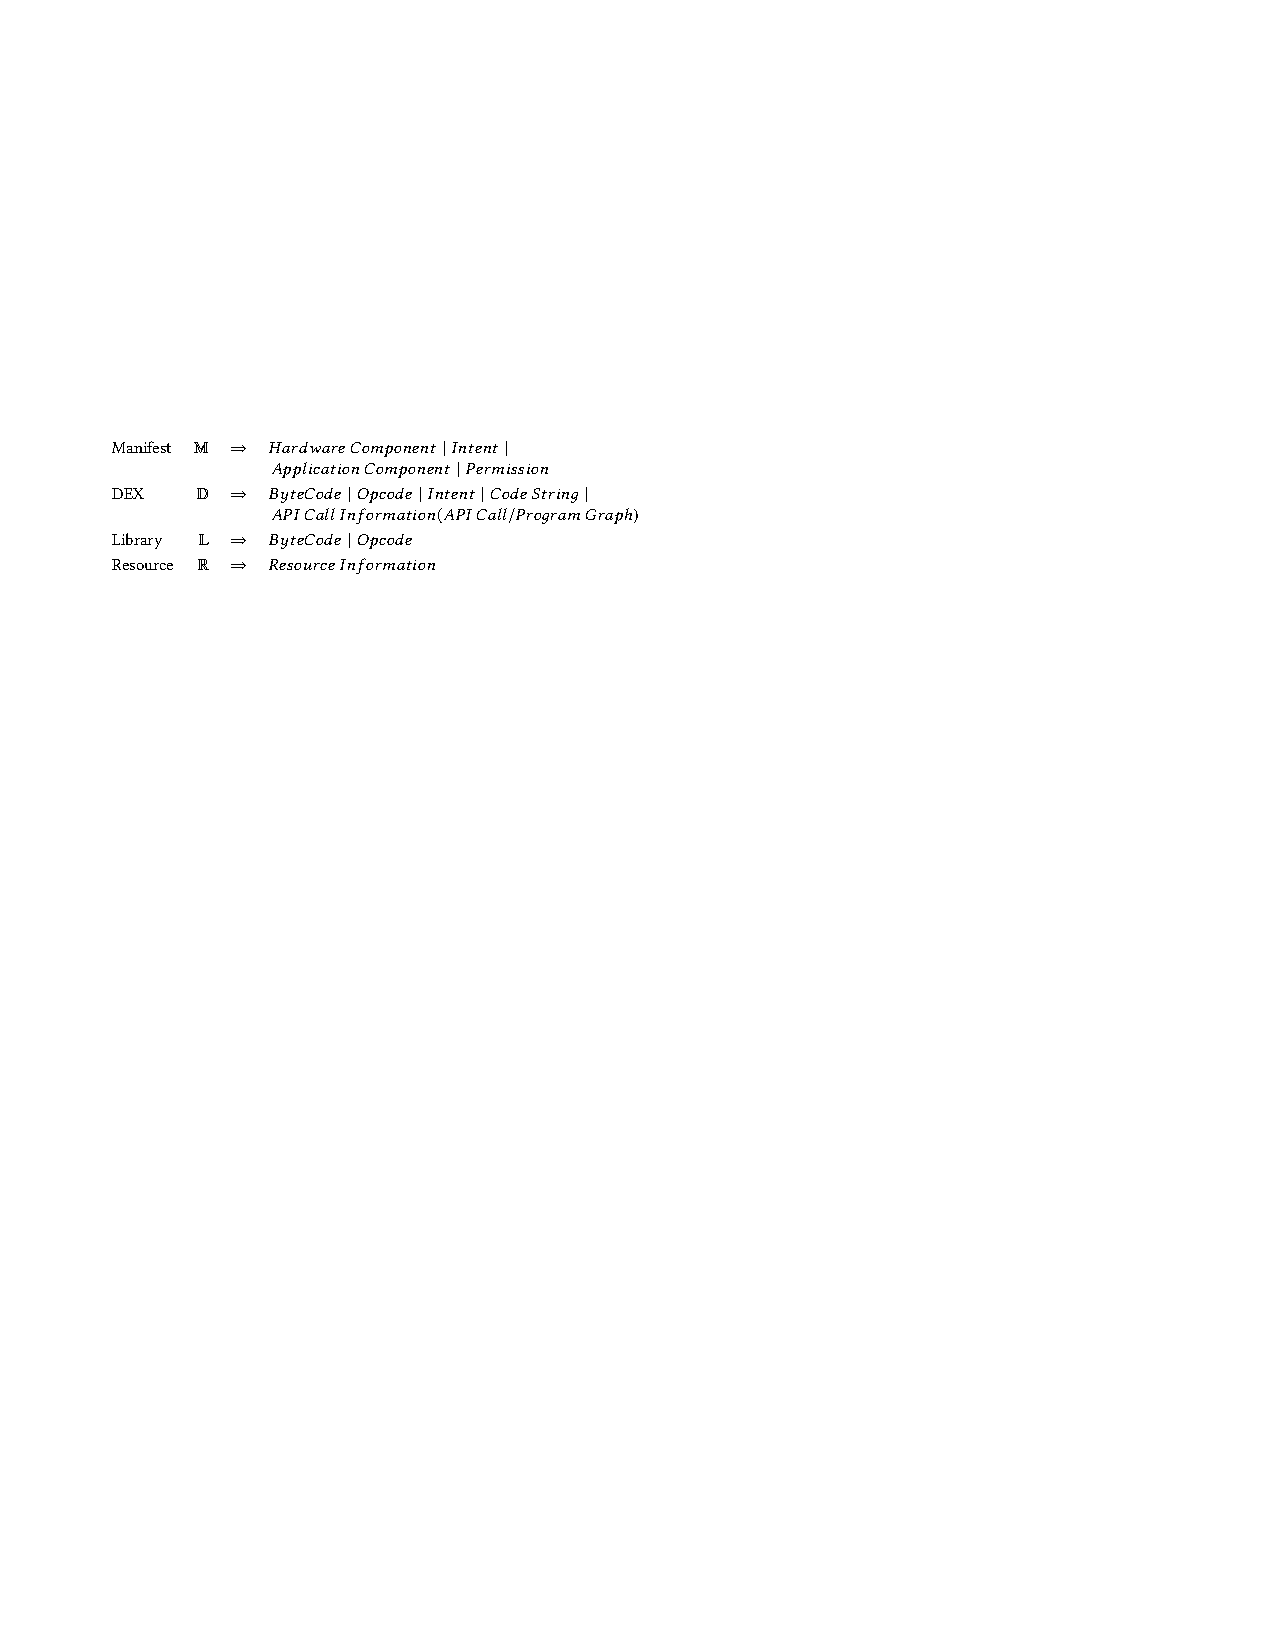
\includegraphics[width=0.68\linewidth]{fig/features.pdf}
    \vspace{-0.2cm}
    \caption{APK files and their corresponding features.}
    \label{fig:features}
    \vspace{-0.6cm}
\end{figure}

\featurepoint{[M|D]}{Intent}
As the primary ways of communication among components, intents connect various Application Components and delineate standard operations one app can perform.
% As the primary ways of communication among components, intents take responsibility for initiating Activities, managing Services lifecycle, and delivering information to Broadcast Receivers.
They are pivotal in initiating Activities, managing Services lifecycle, and delivering broadcast information to Broadcast Receivers.
Malware often monitors these communication status to trigger malicious actions, such as activating pre-configured malicious activities~\cite{zhou2012hey}.
Approaches~\cite{li2021robust,feng2020performance,xu2016iccdetector} aim to capture these malicious behaviors by analyzing corresponding intents.


% Towards this end, intents have been extensively employed to capture potential malicious activities~\cite{feng2020performance,li2021robust,xu2016iccdetector}.

% Approaches like MobiTive~\cite{feng2020performance} and RAMDA~\cite{li2021robust} utilize intents specified in the manifest for malware detection.
% Meanwhile, ICCDetector~\cite{xu2016iccdetector} integrates intents from the manifest and the application's codebase to model the application's behaviors.

\featurepoint{[M]}{Permission}
Android employs a permission-based mechanism to regulate access to sensitive data and restricted actions.
For an app to carry out particular actions, it must obtain the requisite permissions~\cite{au2012pscout,backes2016demystifying}.
The set of permissions required by an app can thus offer insights into its intended behaviors.
Particularly, malware often demands permissions that are unnecessary for benign apps to execute malicious actions~\cite{enck2009lightweight}.
Consequently, numerous Android malware detectors~\cite{he2022msdroid,xu2018deeprefiner,arp2014drebin,kim2018multimodal,wu2021android} capture the differences to distinguish malware. 


% Consequently, numerous malware detection frameworks~\cite{arp2014drebin,xu2018deeprefiner,kim2018multimodal,wu2021android,he2022msdroid} employ permissions as a key heuristic in distinguishing malware.


\featurepoint{[D]}{API Call Information (API Call and Program Graph)}
% \jiahao{Merge API call with its connections}
% \jh{API Call Information is a widely used feature source in Android malware detection, consisting of API calls and their connections.
% Android apps make use of API calls to tap into the operating system's functionality and system resources~\cite{peiravian2013machine}.
% For instance, calling the \textit{sendTextMessage()} indicates that the app is likely to send a text message.
% Additionally, the API calls are often connected with each other to form a program graph, where each node signifies a method, and each edge denotes a method invocation~\cite{li2023black}, illustrating the app's structural information~\cite{wu2019malscan}.}
% \red{For clarity, we decouple API Call Information into two sub-categories: \textit{API Call} refers to the API calls themselves, while \textit{Program Graph} denotes the connections between API calls.}
API Call Information, consisting of API calls and their connections, is a widely utilized feature source in Android malware detection.
Android apps make use of these API calls to access the operating system's functionality and system resources~\cite{peiravian2013machine}.
For instance, the invocation of \textit{sendTextMessage()} suggests that the app is likely to send a text message.
Furthermore, API calls are connected to form a graph, where each node signifies a method, and each edge denotes a method invocation~\cite{li2023black}, illustrating the app's structural information~\cite{wu2019malscan}.
For clarity, we differentiate API Call Information into two sub-categories: \textit{API Call}, referring to the individual API calls, and \textit{Program Graph}, denoting the relationships among these API calls.
Numerous studies~\cite{arp2014drebin,kim2018multimodal,wu2021android} detect sensitive API calls (\textit{e.g., getDeviceId()}) to estimate the probability of an app being malicious.
In contrast, other solutions~\cite{wu2019malscan,he2022msdroid,hou2017hindroid,xu2020sdac,martin2017evolving,ye2019out} venture deeper, examining the relationships between API calls to capture an app's semantics for malware detection.

\featurepoint{[D|L]}{ByteCode and Opcode}
Similar to previous research~\cite{xu2018deeprefiner,sun2016taintart,li2021palmtree,daoudi2021dexray}, we treat both the \textit{raw bytecode} and the \textit{assembly code} derived from the \textit{Dex} and \textit{Library} as ByteCode.
ByteCode contains a sequence of instructions, where each instruction consists of a single Opcode and several operands.
The Opcode denotes a specific operation; for instance, the \texttt{invoke} means a method invocation.
The operands provide additional information for the Opcode, such as the method name.
In addition, ByteCode and Opcode from the \textit{Dex} and \textit{Library} offer insights into the static execution flows of apps' Java and Native codes, providing a view of how an app work~\cite{kim2018multimodal}.
Recent research attempts to represent Bytecode and Opcode in various formats, such as image~\cite{mclaughlin2017deep,hsien2018r2,amin2022android,xiao2019image} and text~\cite{xu2018deeprefiner,yan2018lstm,karbab2021petadroid}, to capture apps' semantics.

% Consistent with previous studies~\cite{xu2018deeprefiner,sun2016taintart,li2021palmtree}, we consider the assembly code derived from the decompilation of DEX and Library files as another kind of bytecode representation of an application.
% Both bytecode and opcode preserve the original characteristics of an application, providing a holistic perspective on the programming behaviors the application executes.

\featurepoint{[D]}{Code String}
Apps often embed key information like URLs and IP addresses as string values within their codebase.
These strings can be traced in the assembly code, tagged either as \texttt{const-string} or \texttt{const-string/jumbo}. 
Such strings can provide crucial clues about potential malicious activities~\cite{arp2014drebin}.
For instance, malware sets up network sockets to communicate with remote servers, using the string \texttt{socket} in the codebase.
A number of works~\cite{arp2014drebin,kim2018multimodal,zhu2019transparent} have used code strings to identify potential illegal operations.

% With the evidence provided by research like~\cite{arp2014drebin,kim2018multimodal,zhu2019transparent}, it is clear that code string has become a significant feature in malware detection.

% Therefore, it is unsurprising that it has been widely adopted as a feature source in Android malware detection~\cite{arp2014drebin,kim2018multimodal,zhu2019transparent}.
% Accordingly, some approaches~\cite{arp2014drebin,kim2018multimodal,zhu2019transparent} have tapped into these strings as indicators for malware detection.

% \featurepoint{[D]}{Program Graph}
% The program graph encapsulates the caller-callee relationships among the methods inside an app as a directed graph, where each node signifies a method, and each edge denotes a method invocation~\cite{li2023black}.
% \jh{In essence, the program graph illustrates the app's structural information, 
% offering a holistic perspective on the app's behavior~\cite{wu2019malscan}.}
% When leveraging program graphs for malware detection, a prevalent strategy is to re-envision them as other constructs (\textit{e.g.}, as a social network) and subsequently employ corresponding techniques to extract valuable insights~\cite{wu2019malscan,wu2021homdroid}.
% Alternatively, some researchers directly apply powerful techniques, like graph neural network (GNN), to distill pertinent information from the program graph itself~\cite{mariconti2016mamadroid,he2022msdroid,gao2021gdroid}.

% To distill helpful information for malware detection, one popular selection is treating the program graph as a social network and apply related techniques to extract information~\cite{wu2019malscan,wu2021homdroid}.
% Another direction is to simplify the graph structure to capture meaningful information~\cite{mariconti2016mamadroid,he2022msdroid}.
% To utilize this information, one direction~\cite{wu2019malscan,wu2021homdroid} treats the program graph as a social network and performs centrality and homophily analysis~\cite{dehghani2016purity,fiore2005homophily}.
% Another direction is to simplify the graph structure to capture meaningful information~\cite{mariconti2016mamadroid,he2022msdroid}.
% There are also some approaches~\cite{} directly extract information from the program graph to detect malware.

% To preserve the program semantic information, MalScan~\cite{wu2019malscan} and HomDroid~\cite{wu2021homdroid} treat the program graph as a social network and perform centrality and homophily analysis~\cite{dehghani2016purity,fiore2005homophily}.

% Also, some approaches have attempted to simplify the graph structure to capture meaningful information. 
% For example, MamaDroid~\cite{mariconti2016mamadroid} abstracts the graph based on family and package details.
% MsDroid~\cite{he2022msdroid} derives subgraphs rooted with sensitive API calls to describe potential malicious operations.

\featurepoint{[R]}{Resource Information}
Apps utilize resources to house traditional files and static elements, such as bitmaps and animation instructions.
These resources are generally decoupled from the application codebase for ease of maintenance.
Attackers sometimes embed malicious code within resource files, like image files, as a tactic to evade detection.
Approaches like DeepRefiner~\cite{xu2018deeprefiner} consider resource information as a crucial feature source for malware detection.
% This stems from the fact that resources typically house traditional and static elements, such as bitmaps and animation instructions. 
% Attackers sometimes embed malicious code within resource files, like image files, as a tactic to evade detection.

% Resources refer to the traditional files and static elements leveraged by your application, such as bitmaps, layout definitions and animation instructions.
% These resources are generally decoupled from the application codebase for ease of maintenance. 
% During runtime, Android selects the most suitable resource based on the device's current configuration
% In some instances, attackers may insert malicious code into resource files, such as image files, as a tactic to elude detection.

% \featurepoint{[DY]}{Dynamic features}
% \jh{dynamic features are collected during runtime, and they are not included in the APK file. For example, the network traffic, the system traces, and the system calls. These information can reflected the app's runtime behaviors. It is time consuming to collect these features.}

\begin{figure}[t]
    \centering
    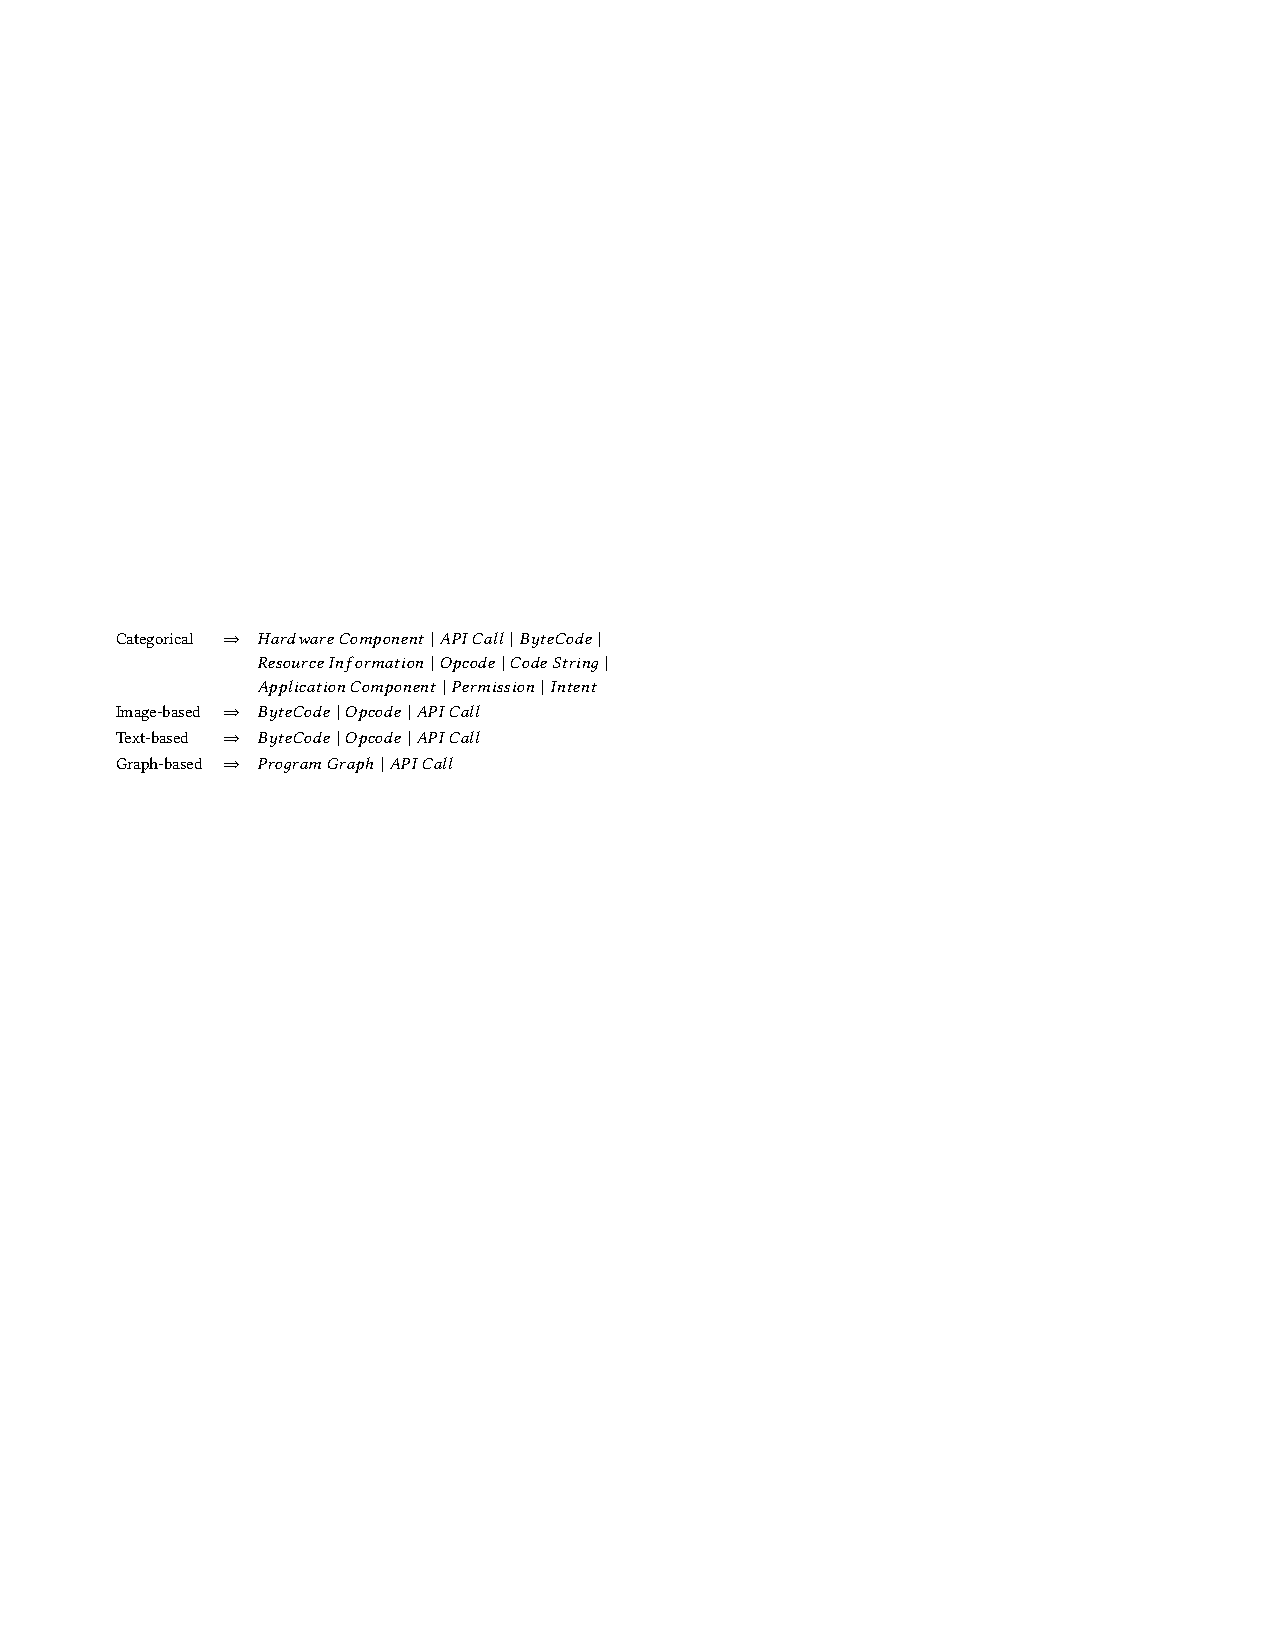
\includegraphics[width=0.68\linewidth]{fig/representation.pdf}
    \vspace{-0.1cm}
    \caption{The relationships between Feature Representations and widely used APK Features.}
    \label{fig:representation}
    \vspace{-0.5cm}
\end{figure}

\subsection{Feature Representation}
\label{sub:apk_feature_encoding}
APK characterizations provide multi-perspective views of an app's behavior.
Before these features can be fed into ML models, they must be encoded into representations that the models can interpret.
Broadly, the encoding process falls into four categories: categorical, image-based, text-based, and graph-based.
\jh{Figure~\ref{fig:representation} illustrates the relationships between these encoding strategies and the corresponding APK features.}
In the following section, we discuss each encoding strategy in detail.

% Some approaches~\cite{yuan2014droid,arp2014drebin,li2019adversarial,feng2019mobidroid,li2021robust,wu2021android,hou2017hindroid} encode these features into a binary vector, where each position indicates whether a specific feature exists or not.
% Alternatively, another approach showcased in~\cite{kim2018multimodal} calculates the frequency of each feature to obtain a vector of real numbers.
\bulletpoint{Categorical encoding}
Features like hardware components, intents, and code strings are often viewed as categorical data and can be easily transformed into numerical values.
A widely-encoding strategy is to convert these features into a binary vector, where each position indicates whether a specific feature exists or not~\cite{arp2014drebin,hou2017hindroid,li2021robust,wu2021android,yuan2014droid,li2019adversarial,feng2019mobidroid}.
On the other hand, another line of research~\cite{kim2018multimodal} calculates the frequency of each feature to obtain a vector of numerical values, reflecting the importance of each feature.

\bulletpoint{Image-based encoding}
% Note: the bytecode definition
% Several approaches~\cite{daoudi2021dexray,ding2020android,mclaughlin2017deep,hsien2018r2,zegzhda2018applying,he2019malware,xiao2019image,yuan2020byte} depict bytecode or opcode sequences in the form of images, subsequently feeding them into a convolutional neural network (CNN) to extract features. 
% In Android malware detection, it is a prevalent practice to represent bytecode or opcode sequences as images.
% Various solutions~\cite{daoudi2021dexray,ding2020android,hsien2018r2,xiao2019image,mclaughlin2017deep} visualize the bytecode or opcode sequences as image forms, subsequently extracting information from these depictions.
% Notably, \textsc{DexRay}~\cite{daoudi2021dexray} transforms the app's bytecode into grey-scale vector images, wherein each pixel corresponds to a distinct byte.
% Additionally, some approaches map various features to images to represent the APK. 
% For instance, Zegzhda et al.~\cite{zegzhda2018applying} attempt to map the sequence of API calls combined with protection levels to an RGB image.
Representing specific features as images and leveraging image processing techniques is a well-established approach in malware detection.
Specifically, bytecode and opcode are often visualized as images to describe apps' behaviors~\cite{mclaughlin2017deep,daoudi2021dexray,hsien2018r2,xiao2019image,ding2020android}.
Notably, \textsc{DexRay}~\cite{daoudi2021dexray} transforms the app's bytecode into grey-scale vector images, wherein each pixel corresponds to a distinct byte.
In a similar vein, some other features are also mapped to images to depict the APK's characteristics.
For instance, Zegzhda et al.~\cite{zegzhda2018applying} combine API calls with protection levels as an RGB image.

\bulletpoint{Text-based encoding}
% Bytecode and opcode sequences can be analogized to textual data.
% Many existing approaches~\cite{xu2018deeprefiner,karbab2018maldozer,karbab2021petadroid,xu2020sdac,sun2019scalable} regard apk characterization as textual data and leverage natural language processing (NLP) techniques to enhance android malware detection.
% By considering API calls as \texttt{words} and their sequences as \texttt{sentences}, methods presented in~\cite{karbab2018maldozer,karbab2021petadroid,xu2020sdac} utilize word embedding techniques, such as Word2Vec~\cite{mikolov2013distributed}, to extract semantic information included in the API calls.
% Separately, Sun et al.~\cite{sun2019scalable} treat API calls and permissions as sparse data, applying Doc2Vec~\cite{le2014distributed} to derive their vector representations.
Text-based encoding is also a widely used strategy in Android malware detection.
Many existing methods~\cite{xu2018deeprefiner,xu2020sdac,karbab2021petadroid,karbab2018maldozer,sun2019scalable} have approached APK features from a textual perspective, employing natural language processing (NLP) techniques to amplify detection capability.
For example, by considering API calls as \texttt{words} and their sequences as \texttt{sentences}, methods presented in~\cite{xu2020sdac,karbab2021petadroid,karbab2018maldozer} utilize word embedding techniques, such as Word2Vec~\cite{mikolov2013distributed}, to extract semantic information included in the API calls.
Separately, Sun et al.~\cite{sun2019scalable} treat API calls and permissions as sparse data, applying Doc2Vec~\cite{le2014distributed} to derive their vector representations.

\bulletpoint{Graph-based encoding}
Recently, graph structure has been widely adopted to represent apps' semantics~\cite{he2022msdroid,li2023black}.
One direction is to leverage program graphs to model APK behaviors~\cite{wu2019malscan,wu2021homdroid,he2022msdroid,pektacs2020deep,pektacs2020learning}.
Another avenue aims to build API-based feature graphs, drawing insights from API calls and their meta-relationships. 
An example is to identify whether two API calls are in the same block, thereby capturing the app's intended operations~\cite{hou2017hindroid,huang2019deep}.
When these features are represented as graphs, graph-based techniques (\textit{e.g.,} Graph2Vec~\cite{narayanan2017graph2vec}, social network~\cite{wu2019malscan}) are employed to extract apps' structural information.



% \vspace{-0.1cm}
\subsection{Machine Learning Modeling}
\label{sub:ml_models}
% Subsequent to encoding, learning models are leveraged to identify underlying patterns from the encoded features, facilitating informed predictions.
After encoding these features as numerical vectors, machine learning models are leveraged to identify malicious patterns.
Following previous studies~\cite{qiu2020survey,zhao2021impact}, we categorize the models employed in Android malware detection into two main categories: traditional machine learning (TML) and deep learning (DL) models.
TML models, such as linear regression or decision trees, typically exhibit simpler structures that can explicitly model the relationship between input and output. 
As such, these TML models often require domain knowledge to extract features from input data.
In contrast, DL models are characterized by their multiple layers of neurons, enabling them to capture complex non-linear mappings from input to output~\cite{zhao2018deepsim}.
This capability means that DL models are less reliant on domain knowledge during the feature extraction.
In this section, we provide a concise introduction to the widely used models.
%  in Android malware detection.

\bulletpoint{TML models}
% SVM~\cite{arp2014drebin,hou2017hindroid,xu2020sdac,sun2016sigpid,garcia2018lightweight}
% KNN~\cite{wu2019malscan,wu2021homdroid,wu2016effective,aafer2013droidapiminer}
% RF~\cite{mariconti2016mamadroid,zhu2018hemd}
% DT~\cite{zarni2013permission,yerima2014android}
% (SVM)~\cite{noble2006support}
% (KNN)~\cite{peterson2009k} (RF)~\cite{breiman2001random}
Given APK features, TML models are commonly employed to discern patterns from them.
The Support Vector Machine (SVM) can find one hyperplane that separates the high-dimensional data points with varying labels.
This capability has made it a popular choice to detect Android malware~\cite{arp2014drebin,hou2017hindroid,xu2020sdac,sun2016sigpid,garcia2018lightweight}.
K-Nearest Neighbors (KNN) has also been applied in Android malware detection~\cite{wu2019malscan,wu2021homdroid,aafer2013droidapiminer,wu2016effective}.
This algorithm identifies the nearest neighbors of a given sample and subsequently classifies the sample based on the majority label of its neighbors.
Additionally, as an ensemble-based learning method, Random Forest (RF) creates a forest of decision trees, each trained on a random subset of the data.
This approach capitalizes on the strength of multiple decision trees, making the model more robust and accurate than individual trees.
Such advantages have led to its significant application in malware detectors~\cite{mariconti2016mamadroid,zhu2018hemd}.

\bulletpoint{DL models}
DL models have exhibited strong capability in modeling malware behaviors. 
This part provides an insight into the widely used DL models tailored for Android malware detection.
% Multi-Layer Perceptron (MLP) is a fundamental model composed of multiple layers of neurons and has been applied in various studies~\cite{kim2018multimodal,li2021robust,martin2017evolving,sun2019scalable,zhu2019fsnet,chen2020denas}.
As a basic feed-forward neural network, Multi-Layer Perceptron (MLP), composed of several layers of neurons, \jh{has shown significant effectiveness in detecting Android malware~\cite{kim2018multimodal,li2021robust,martin2017evolving,sun2019scalable,zhu2019fsnet,chen2020denas}.}
The Recurrent Neural Network (RNN)~\cite{medsker2001recurrent} is a type of neural architecture that can capture the sequential information of input data.
By representing APK features (\textit{e.g.}, API calls and bytecode) as sequences, existing solutions~\cite{xu2018deeprefiner,yan2018lstm,vinayakumar2017deep} leverage RNN to explore the temporal dependencies embedded in these features.
The Convolutional Neural Network (CNN)~\cite{he2017mask} is equipped with multiple convolutional and pooling layers, enabling it to recognize contextual information derived from low-level features~\cite{girshick2015fast}.
This intrinsic capability makes it especially effective in capturing patterns from image-oriented data.
Reflecting its efficacy, CNN has been extensively employed to extract malicious patterns from image-based features in Android malware detection~\cite{mclaughlin2017deep,hsien2018r2,feng2019mobidroid,karbab2018maldozer,huang2019deep,he2019malware}.
Given the graph representation of APK features (\textit{e.g.,} program graphs), Graph Neural Network (GNN)~\cite{kipf2016semi} can facilitate malware detection~\cite{he2022msdroid,mariconti2016mamadroid,gao2021gdroid,fan2021heterogeneous}.
This is because GNN can effectively propagate and aggregate node information along graph edges, thereby capturing the structural information of apps.
% some approaches~\cite{he2022msdroid,gao2021gdroid,fan2021heterogeneous} have attempted to tailor Graph Neural Networks (GNN) to facilitate malware detection.
Utilizing a process of encoding and subsequently decoding input features, Autoencoders (AE) have the capacity to generate refined data representations, which makes it a popular choice in detecting malware~\cite{li2021robust,yang2021cade,zhu2021hybrid}.

In addition, existing research~\cite{su2016deep,wang2020sedroid,amin2022android} also tries to explore the potential of other DL models, like generative adversarial network (GAN)~\cite{goodfellow2014generative} and deep belief network (DBN)~\cite{hinton2009deep}.
For instance, Amin et al.~\cite{amin2022android} employ the dual-network structure of GAN --- one generates malware samples and the other works to distinguish these samples --- to enhance the malware detection capability.


% \begin{center}
%     \begin{conclusionbox}
%     \textit{Finding:} 
%     \jh{Central to static and ML-based Android malware detection is how to effectively \textit{profile apps' behaviors} and how to \textit{leverage suitable ML models} to unveil malicious patterns.}
%     \end{conclusionbox}
% \end{center}

\begin{center}
    \begin{conclusionbox}
    \textit{Finding:} 
    \jh{At the core of static and ML-based Android malware detection lies the ability to accurately \textit{profile app behaviors} and to \textit{select and leverage appropriate ML models} that can effectively uncover malicious patterns. Achieving this requires not only expressive feature representations but also a careful alignment between behavioral semantics and model capabilities.}
    \end{conclusionbox}
\end{center}

% \subsection{Summary}
% \label{sub:summary}
% Quick summarize this section, and use some motivation to illustrate we need to conduct a quantitative analysis on the primary techniques.


% \begin{table*}[t]
% \centering
% \caption{
% % (\textit{AndroidManifest.xml} for Manifest, \textit{classes*.dex} for Dex, \textit{res/*} for Resource, and \textit{*.so} for Library)
% An overview of the 12 representative approaches we selected from major venues in security, software engineering, and machine learning. 
% \ymark \ indicates that the APK file (e.g., \textit{AndroidManifest.xml} for Manifest) is taken as input in Android malware detection, while \nmark \ is the opposite.
% \cmark \ and \xmark \ indicate whether feature engineering is handcrafted using domain knowledge or learned using representation learning.
% The effectiveness we present is based on the results reported in the original papers.}
% \begin{adjustbox}{width=0.85\linewidth}
% \begin{tabular}{@{}c|cc|cccc|cc|rr|rrr@{}}
% \toprule
% \multirow{2}{*}{\raisebox{-0.3cm}{\textbf{\begin{tabular}[c]{@{}c@{}}Selected \\ Approach\end{tabular}}}} & \multicolumn{2}{c|}{\textbf{Publication}} & \multicolumn{4}{c|}{\textbf{Input from APK}} & \multicolumn{2}{c|}{\textbf{Feature Engineering}} & \multicolumn{2}{c|}{\textbf{Dataset}} & \multicolumn{3}{c}{\textbf{Effectiveness}} \\ \cmidrule(lr){2-3} \cmidrule(lr){4-7} \cmidrule(lr){8-9} \cmidrule(lr){10-11} \cmidrule(l){12-14}
%  & \textbf{Venue} & \textbf{Year} & \textbf{Manifest} & \textbf{Dex} & \textbf{Resource} & \textbf{Library} & \textbf{Handcrafted} & \textbf{Learned} & \textbf{Malware} & \textbf{Goodware} & \textbf{TPR} & \textbf{FPR} & \textbf{F1} \\ \midrule
% Drebin\cite{arp2014drebin} & NDSS & 2014 & \ymark & \ymark & \nmark & \nmark & \cmark & \xmark & 5,560 & 123,453 & 94\% & \textbf{1\%} & 87\% \\ \midrule
% % ICCDetector\cite{xu2016iccdetector} & TIFS & 2016 & \ymark & \ymark & \nmark & \nmark & & & 5,264 & 12,026 & 93\% & \textbf{1\%} & 96\% \\ \midrule
% MamaDroid\cite{mariconti2016mamadroid} & NDSS & 2017 & \nmark & \ymark & \nmark & \nmark & \cmark & \xmark & 35,493 & 8,447 & 97\% & 2\% & 96\% \\ \midrule
% Mclaughlin et al.\cite{mclaughlin2017deep} & CODASPY & 2017 & \nmark & \ymark & \nmark & \nmark & \xmark& \cmark & 13,637 & 13,758 & 95\% & \textbf{1\%} & 97\% \\ \midrule
% HinDroid\cite{hou2017hindroid} & KDD & 2017 & \nmark & \ymark & \nmark & \nmark & \cmark & \xmark & 1,216 & 1,118 & \textbf{99\%} & 2\% & \textbf{99\%} \\ \midrule
% DeepRefiner\cite{xu2018deeprefiner} & EuroS\&P & 2018 & \ymark & \ymark & \ymark & \nmark & \xmark & \cmark & 62,915 & 47,525 & 98\% & 2\% & 98\% \\ \midrule
% Kim et al.\cite{kim2018multimodal} & TIFS & 2018 & \ymark & \ymark & \nmark & \ymark & \cmark & \cmark & 21,260 & 20,000 & \textbf{99\%} & \textbf{1\%} & \textbf{99\%} \\ \midrule
% MalScan\cite{wu2019malscan} & ASE & 2019 & \nmark & \ymark & \nmark & \nmark & \cmark & \xmark & 15,430 & 15,285 & --- & --- & 98\% \\ \midrule
% SDAC\cite{xu2020sdac} & TDSC & 2020 & \nmark & \ymark & \nmark & \nmark & \xmark & \cmark & 34,497 & 35,645 & 98\% & \textbf{1\%} & \textbf{99\%}\\ \midrule
% HomDroid\cite{wu2021homdroid} & ISSTA & 2021 & \nmark & \ymark & \nmark & \nmark & \cmark & \xmark & 3,358 & 4,840 & 97\% & 4\% & 95\% \\ \midrule
% Xmal\cite{wu2021android} & TOSEM & 2021 & \ymark & \ymark & \nmark & \nmark & \cmark & \xmark & 15,570 & 20,120 & 98\% & 2\% & 98\% \\ \midrule
% RAMDA\cite{li2021robust} & WWW & 2021 & \ymark & \ymark & \nmark & \nmark & \cmark & \xmark & 21,621 & 36,862 & 93\% & \textbf{1\%} & 90\% \\ \midrule
% MSDroid\cite{he2022msdroid} & TDSC & 2022 & \nmark & \ymark & \nmark & \nmark & \cmark & \xmark & 30,210 & 51,580 & 97\% & \textbf{1\%} & 97\% \\ \bottomrule
% \end{tabular}
% \end{adjustbox}
% \centering
% \begin{tablenotes}
% \footnotesize
% \item \ \ TPR, FPR, and F1 refer to true positive rate, false positive rate, and F1-score. 
% As MalScan is only evaluated on F1, its TPR and FPR are not available.
% \end{tablenotes}
% \label{tab:literature}
% \vspace{-0.4cm}
% \end{table*}

\section{\codename}
\label{sec:framework}

% The architecture of \codename is depicted in Figure~\ref{fig:framework}. 
% Beginning with a dataset of Android apps, the first step is to extract pertinent features from these apps.
% These features are then meticulously stored in a feature database. More details are provided in~\ref{sub:feature_db}.
% Subsequently, a dedicated preprocessor is utilized to transform (including retrieving and encoding) these features.
% After that, we proceed to train an ML model and assess its performance in detecting malware.

% % The framework is crafted with two guiding principles at its core: modularization and flexibility.
% \codename is designed with modularity in mind, making it easy to extend and customize.
% This is achieved by decoupling it into three distinct modules: \textit{feature database}, \textit{preprocessor}, and \textit{ML model}.
% Given the structured format of the \textit{feature database}, one can easily incorporate new features and integrate them into the assessment pipeline.
% Moreover, the \textit{preprocessor} can be tailored to accommodate various approaches, granting users the flexibility to determine what/how features are used.
% The \textit{ML model} is preloaded with various ML models, such as SVM, MLP, CNN, and AE.
% Alternatively, \codename also supports custom models, allowing users to incorporate their own models into the framework.

% \begin{figure}[t]
%     \centering
%     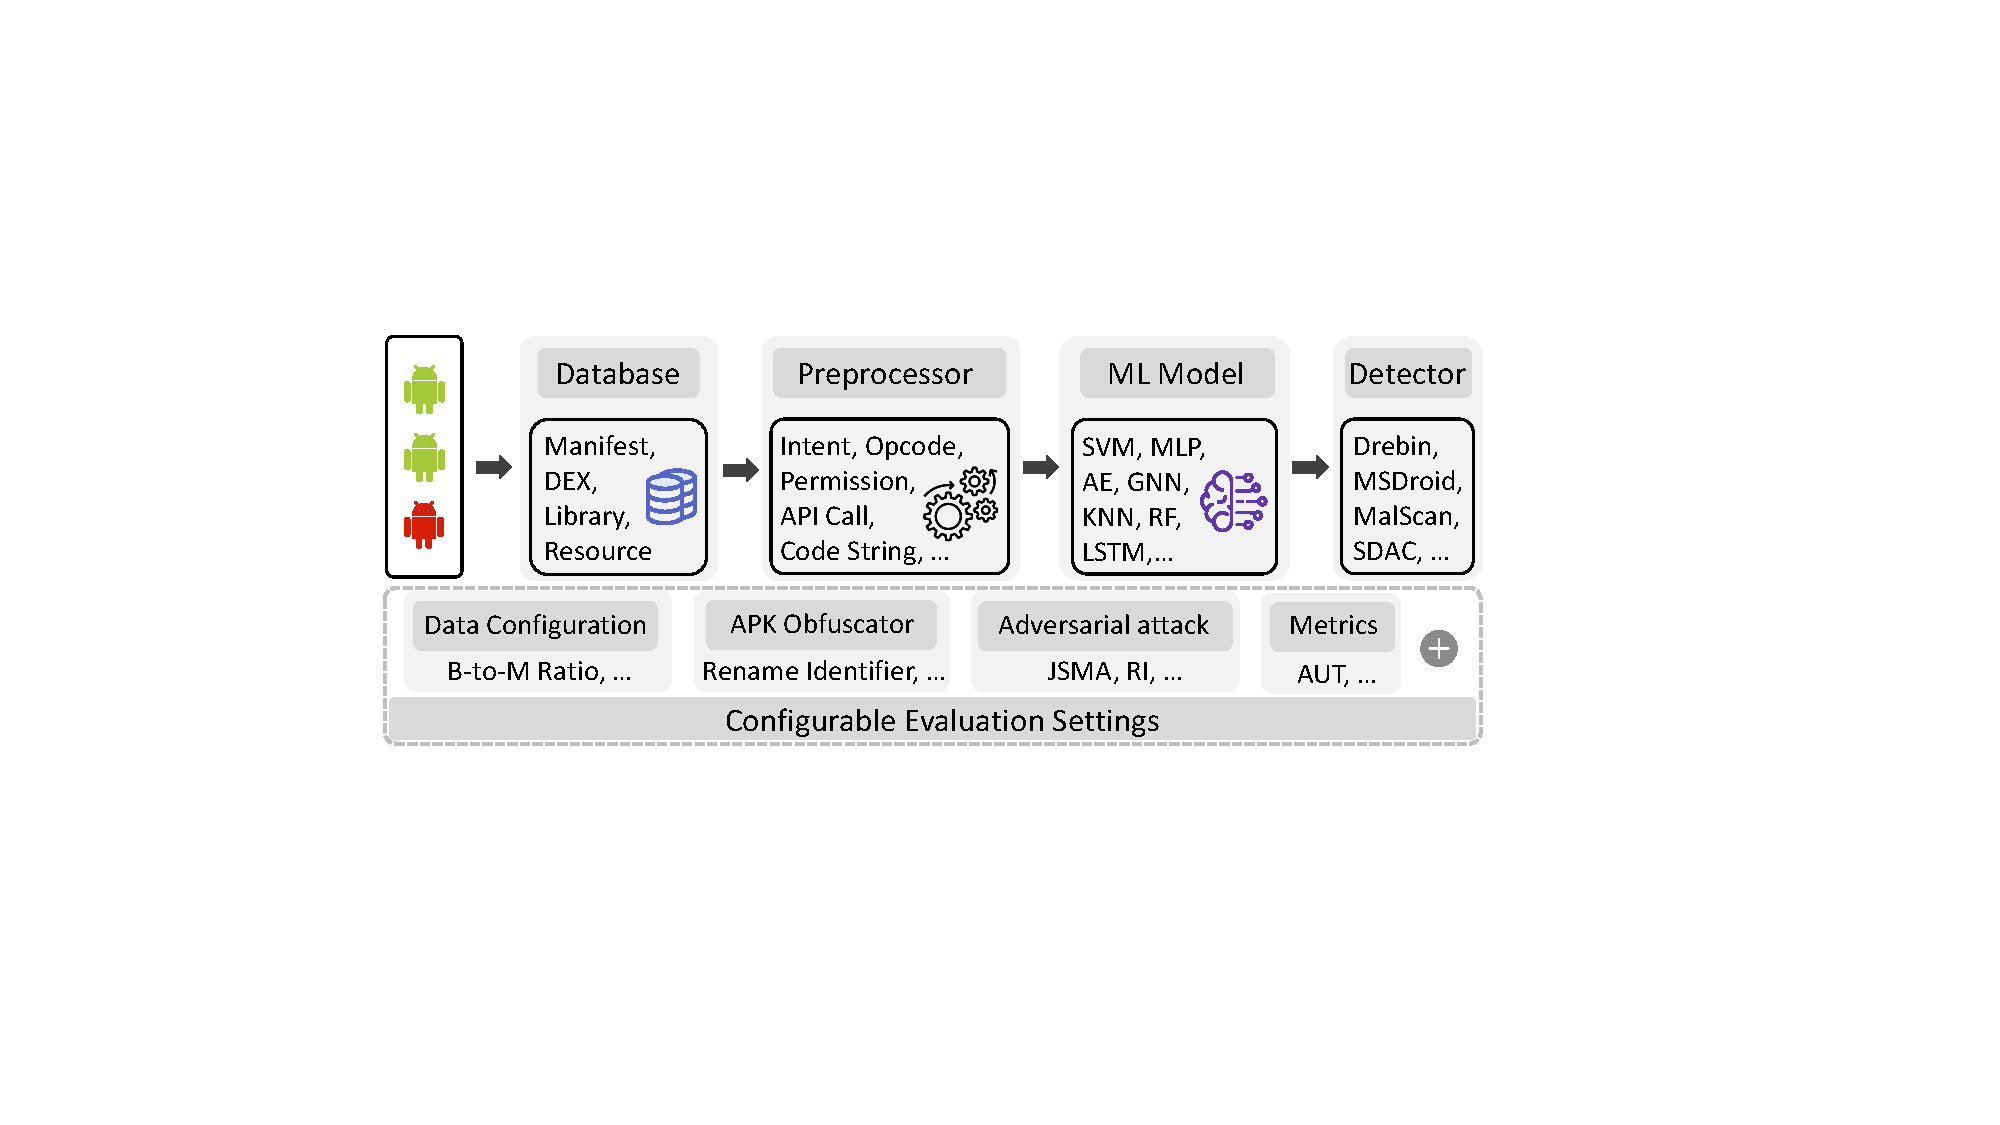
\includegraphics[width=0.94\linewidth]{fig/framework.pdf}
%     \caption{The architecture of \codename.}
%     \label{fig:framework}
%     % \vspace{-0.6cm}
% \end{figure}

% % Following the feature storing format in the {\em feature database}, it is easy to aggregate new features into the framework.
% % With this design, it is easy to design an additional feature extractor and store the derived features in the {\em feature database}, ensuring a smooth integration into the assessment pipeline.
% % Additionally, the {\em preprocessor} can be tailored to accommodate various approaches, granting users the flexibility to choose and adapt feature usage as required.
% \codename also provides a configurable experimental setting to support a wide range of evaluation scenarios.
% Parameters such as the ratio of goodware-to-malware, training data sizes, and time decay are all adjustable.
% This enables users to meticulously select APK samples for diverse evaluation contexts, ensuring comprehensive and accurate assessments.
% Moreover, \codename integrates an APK obfuscator~\cite{aonzo2020obfuscapk}, allowing for obfuscation prior to feature extraction. 
% It also possesses the capability to produce adversarial samples, enabling a robust assessment of model resilience.
% % Leveraging the capabilities of \codename, we re-implement the approaches described in Section~\ref{sec:approach_analysis} and assess them with our curated dataset.
% % We further analyze the evaluation outcomes to provide deeper insights into the current ML-based Android malware detection in Section~\ref{sec:evaluation}.

% % \bulletpoint{Implementation}
% % \codename is developed in 17K lines of Python code.
% % To ensure consistency and mitigate biases from different feature extraction toolchains and learning frameworks, we adopt standardized techniques across all tasks.
% % For feature extraction, we use Androguard to disassemble APK files and derive features such as permissions, intents, and program graphs. 
% % LibRadar helps in identifying third-party libraries within the applications, while Angr is used for analyzing native libraries and capturing essential features like opcodes and API calls. 
% % When it comes to training ML models, the scikit-learn library is our choice for traditional ML algorithms like SVM, KNN, and RF.
% % On the other hand, for DL architectures such as CNN, LSTM, GNN, and AE, we resort to Pytorch.
% % This uniform approach ensures a balanced evaluation, concentrating purely on the uniqueness and performance of each method.
% % Details about the hyper-parameters of these models are provided in Appendix~\ref{sub:hyperparameters}.

\begin{figure}[t]
    \centering
    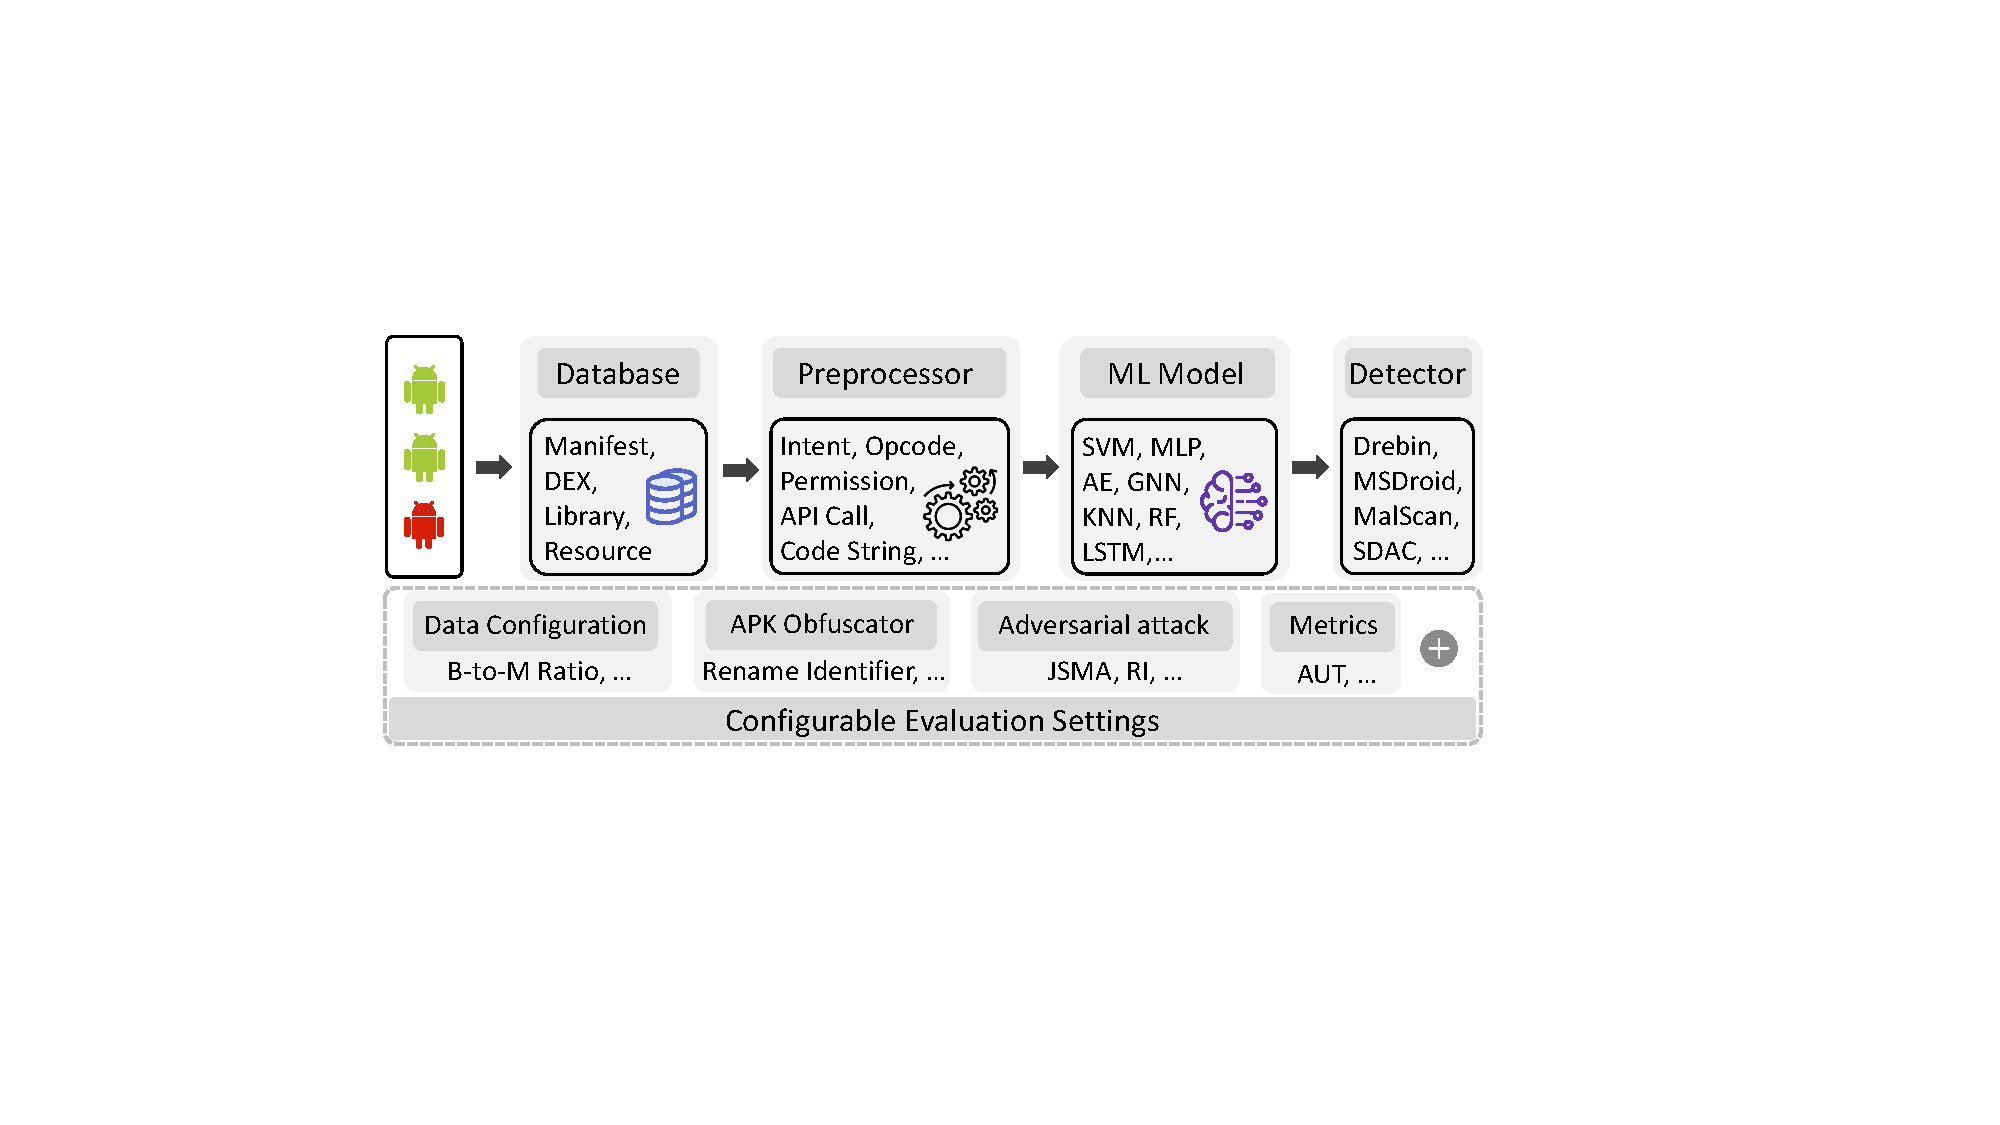
\includegraphics[width=0.74\linewidth]{fig/framework.pdf}
    \vspace{-0.1cm}
    \caption{The architecture of \codename.}
    \label{fig:framework}
    \vspace{-0.3cm}
\end{figure}

% Having analyzed existing ML-based Android malware detection approaches, we propose a general-purpose framework, \codename, to facilitate the development and evaluation of new Android malware detectors.

To support experimental reproducibility and fair comparison, we propose a general-purpose framework, \codename, guided by the detection workflow discussed in Section~\ref{sec:systematic_investigation}, to facilitate the development and evaluation of new Android malware detectors.
Figure~\ref{fig:framework} illustrates the overall architecture and workflow of \codename.
% It starts with a collection of apps, from which a set of features is extracted and stored in a {\em feature database}.
The process begins with a collection of apps, from which a set of features is extracted and stored in a {\em feature database}.
These features are then processed by a {\em preprocessor}, which transformes them into numerical vectors.
A selected {\em ML model} is subsequently trained and evaluated to detect malicious applications.
Furthermore, \codename provides configurable experimental settings to support diverse real-world scenarios, such as varying goodware-to-malware ratios, different training data sizes, and robustness assessments against adversarial attacks.
% It is implemented in 17K lines of Python code, detailed in Appendix~\ref{sub:implementation}.
%
% The framework is crafted with two guiding principles at its core: modularization and flexibility.
% \jh{\codename is modular, which makes it easy to extend and customize according to various requirements.}
% This is achieved by decoupling it into three modules: \textit{feature database}, \textit{preprocessor}, and \textit{ML model}.
% Given the structured format of the \textit{feature database}, one can easily incorporate new features and integrate them into the assessment pipeline.
% Moreover, the \textit{preprocessor} can be tailored to accommodate various approaches, granting users the flexibility to determine what/how features are used.
% The \textit{ML model} is preloaded with various ML models, such as SVM, MLP, CNN, and AE.
% Alternatively, \codename also supports custom models, allowing users to incorporate their own models into the framework.
% Given the structured format of the \textit{feature database} (details can be found in~\ref{sub:feature_db}), one can easily incorporate new features and integrate them into the assessment pipeline.

This modular design of \codename simplifies the development of ML-based Android malware detectors. Three key modules, \textit{feature database}, \textit{preprocessor}, and \textit{ML model}, captures the main aspects of designing ML solutions for Android malware detection.
% \textit{Feature database} organizes the extracted features categorically, including Manifest, ProgramGraph, DisassembledCode, and SharedLibrary, which can be easily extended to incorporate new features.
The \textit{feature database} organizes extracted features categorically according to their sources, as discussed in Section~\ref{sub:apk_characterization}, including Manifest, Dex, Library, and Resource. 
For example, the Manifest category contains features extracted from the AndroidManifest.xml file, such as permissions, intents, and application components.
Further details about the feature database are provided in Appendix~\ref{sub:feature_db}.
Notably, all features are stored in a manner consistent with our APK characterization taxonomy.
Each directory corresponds to a specific feature source, and the features of a given APK are distributed accordingly --- for instance, Hardware Components and Application Components under Manifest; API Calls, Opcodes, and Program Graphs under Dex; Native Functions under Library; and Image Resources under Resource.
Such structured storage enables developers to easily query and extract the required features without re-extracting them from the original APKs, greatly accelerating the development of new detectors.
% For example, users can quickly retrieve a subset of features from the database at the APK characterization level when designing a new detector with \textit{preprocessor}.
In addition, the modular design allows new feature types to be seamlessly integrated into the framework.

The \textit{preprocessor} retrieves and encodes features before they are fed into the ML model.
This module can be customized to support different detectors, providing flexibility in feature selection and usage.
Leveraging the structured organization of the \textit{feature database}, users can easily select and combine features from multiple sources to construct customized feature vectors.
For instance, when designing a new detector, one can quickly retrieve a subset of features at the APK-characterization level using the \textit{preprocessor}.
To replicate a detector that relies on API calls and permissions, the \textit{preprocessor} can be configured to extract these features from the Dex and Manifest categories, respectively, and encode them into a unified feature vector.

The \textit{ML model} module integrates a wide range of commonly used machine learning models, such as RF, SVM, KNN, MLP, LSTM, CNN, GNN, and AE.
Each model offers user-friendly interfaces for training, testing, and evaluation, and the module supports easy customization and extension --- for example, adding new neural network architectures.
To develop a new detector, users only need to customize the \textit{preprocessor} to select the required features from the \textit{feature database} and feed them into the chosen model within the \textit{ML model} module.
If certain features or models are not yet supported, the framework can be readily extended by adding new feature types to the \textit{feature database} and incorporating additional learning models into the ML module.


\codename provides configurable experimental settings to support different evaluation scenarios.
Parameters, such as, training sample size, goodware-to-malware ratios, and temporal distribution of samples, are all adjustable.
The framework offers fine-grained control over these parameters and supports checkpointing during both training and evaluation.
This flexibility facilitates app selection and scenario construction, ensuring comprehensive and accurate evaluations.
For example, users can configure the goodware-to-malware ratio to assess model performance under varying malware prevalence.
They can also adjust the temporal distribution of apps to simulate malware evolution, which is essential for evaluating model robustness.
Furthermore, with flexible training-sample configuration and organized checkpoint management, \codename enables incremental training, allowing users to incorporate new training samples and continue training from existing models.

% \codename offers fine-grained control over these parameters and support checkpointing during training and evaluation.
% This facilitates app selection to construct diverse scenarios, ensuring comprehensive and accurate evaluation.
% For instance, one can configure the ratio of goodware-to-malware to evaluate the model's performance under different malware prevalence.
% We can adjust the apps distribution over time to simulate the evolution of malware, which is crucial for assessing the model's robustness.
% Given the flexibility to adjust training samples and categorize model checkpoints, \codename also enables incremental training, allowing users to add new training samples and continue training from existing models. 

\codename also integrates an APK obfuscator~\cite{aonzo2020obfuscapk}, which can produce various types of obfuscated samples, \textit{e.g.}, identifier renaming, resource encryption, code modification, and invocation reflection.
Obfuscation is applied to APKs before feature extraction to generate their obfuscated variants.
The different obfuscation types can be applied as independent operations: one can first apply one type of obfuscation and then apply another to an already obfuscated APK. 
This capability is essential for evaluating the model's resilience to obfuscated malware.
Moreover, this framework incorporates an adversarial sample generation mechanism from AndroidHIV~\cite{chen2019android}, enabling the assessment of model resilience to adversarial attacks.
Specifically, adversarial samples are generated by perturbing the feature vectors of original samples, and these perturbed samples are then used to evaluate the robustness of the trained models.
The perturbation process ensures that the functionality of the original apps is preserved.
Further details can be found in AndroidHIV~\cite{chen2019android}.
Such flexibility and adaptability make \codename a versatile tool for developing and evaluating ML-based Android malware detectors.


% \tosem{Add discussion about the training methods, such as incremental training, only need to add new training samples, and load existing models for further traning.
% As for the obfuscation techniques, our framework re-parses the apks, can support the concurrently, if applying them to the apks.}



% The implementation of \codename is in the Appendix~\ref{sub:implementation}.


% \bulletpoint{\codename Implementation}
% \codename is developed in 17K lines of Python code.
% To ensure consistency and mitigate biases from different feature extraction toolchains and learning frameworks, we adopt standardized techniques across all tasks.
% For feature extraction, we use Androguard~\cite{androguard} to disassemble APK files and derive features such as permissions, intents, and program graphs. 
% LibRadar~\cite{libradar} helps in identifying third-party libraries within the applications, while Angr~\cite{angr} is used for analyzing native libraries and capturing essential features like opcodes and API calls. 
% When it comes to ML models, the scikit-learn library is our choice for traditional ML algorithms like SVM, KNN, and RF.
% On the other hand, for DL architectures such as CNN, GNN, and AE, we resort to Pytorch~\cite{pytorch}.
% This uniform approach ensures a balanced evaluation, concentrating purely on the uniqueness and performance of each method.

\bulletpoint{\codename Implementation}
\codename is developed in 17K lines of Python code.
To ensure consistency and mitigate biases from different feature extraction toolchains and learning frameworks, we adopt a standardized setup across all Android malware detectors.
For feature extraction, we use Androguard~\cite{androguard} to disassemble APK files and derive features such as permissions, intents, and program graphs. 
LibRadar~\cite{libradar} helps in identifying third-party libraries within the applications, while Angr~\cite{angr} is used for analyzing native libraries and capturing essential features like opcodes and API calls. 
When it comes to machine learning models, the scikit-learn library is our choice for traditional ML algorithms like SVM, KNN, DT and RF.
On the other hand, for deep learning architectures such as CNN, GNN, and AE, we resort to Pytorch~\cite{pytorch}.
This uniform approach ensures a balanced evaluation, concentrating purely on the uniqueness and performance of each method.
\tosem{Currently, we make \codename available to interested researchers upon request.
It has already been adopted by several academic and industrial organizations in countries such as the US, Germany, Singapore, and China for developing and evaluating ML-based Android malware detectors.
This adoption demonstrates its practicality and effectiveness in supporting malware analysis research.}
We plan to release \codename publicly to further facilitate future work in this domain.
\vspace{-0.1cm}
\section{Representative Approach Analysis}
\label{sec:approach_analysis}

% To understand the state of ML-based Android malware detection, a quantitative analysis of current work is indispensable.

% With the rapid evolution of this field, hundreds of techniques have been proposed and achieved remarkable performance in the past decade.
% A systematic investigation of relevant works dating back to 2011 is discussed in Sec.~\ref{sec:discussion} to highlight extensive efforts that have been devoted to Android malware detection.

% While an ideal scenario is evaluating as many approaches as possible, conducting an exhaustive examination of each method is impractical due to the vast amount of existing literature.

% Moreover, it is important to know that, despite the abundance of publications in this area, many papers present slight variations of similar techniques, and novel solutions are comparatively fewer.
% Moreover, it is important to understand that, despite vast publications in this area achieving promising results, many of them share similar techniques (\textit{e.g.,} similar neural networks), and novel solutions are comparatively fewer.

% Thus, our analysis focuses on methods that represent the broad spectrum and depth of advancements in the field.
% In the section, we first outline the selection principles and provide a summary of the selected approaches.
% Then, a comparative analysis is presented to offer insights into the experimental designs.

To understand the state of ML-based Android malware detection, a quantitative analysis of current work is indispensable.
While an ideal scenario is evaluating as many approaches as possible, conducting an exhaustive examination of each method is impractical due to the vast amount of existing literature.
Moreover, it is important to understand that, despite vast publications in this area achieving promising results, many of them share similar techniques (\textit{e.g.,} similar neural networks), and novel solutions are comparatively fewer.
Thus, our analysis focuses on methods that represent the broad spectrum and depth of advancements in the field.
That is, we aim to select representative approaches and utilize our framework to re-implement and evaluate them.
Specifically, in this section, we outline the selected approaches and provide a comparative analysis to highlight their experimental designs.
We then quantitatively evaluate these approaches in Section~\ref{sec:evaluation}, shedding further light on the current state of ML-based Android malware detection.

% In the section, we first outline the selection principles and provide a summary of the selected approaches.
% Then, a comparative analysis is presented to offer insights into the experimental designs.

\subsection{Selection Criteria}
\label{sub:selection_criteria}

\bulletpoint{Cover various communities}
Android malware detection stands as an interdisciplinary domain, drawing contributions from diverse communities, including software engineering, security, and machine learning.
However, a notable separation is observed --- the solutions in one community often only compare with others from the same community --- which hinders potential collaborative advancements.
For instance, methods like~\cite{hou2017hindroid,ye2019out} from one community are often evaluated in isolation, complicating direct performance comparison.
To bridge the gap, we incorporate approaches from leading venues across a broad range of communities.
% To address this, we select approaches from a range of communities.

% This includes various mixes of APK features, feature representations, and ML models.
\bulletpoint{Explore an extensive spectrum of techniques in the detection pipeline}
As identified in Sec.~\ref{sec:systematic_investigation}, a wide range of technique combinations exists across different phases of the detection pipeline.
This study explores as many techniques as possible in each phase, including various mixes of APK features, feature representations, and ML models.
Such a comprehensive investigation enables us to gain a thorough understanding of the entire workflow of ML-based Android malware detection.

% \jh{This study explores these stages, examining various mixes of APK features, feature representations, and ML models.
% Such a comprehensive investigation enables us to gain a thorough understanding of the entire workflow of Android malware detection.}

\bulletpoint{Reflect research progress}
% Considering the evolving landscape of this field, where novel methods continually emerge, we prioritize approaches that introduce new techniques or achieve remarkable performance, such as proposing new feature representations or employing new learning architectures.
In consideration of the evolving research landscape, where new methodologies continually emerge, we place emphasis on approaches that introduce cutting-edge techniques.
Particularly, we prioritize methods that either propose novel feature representations or employ innovative learning architectures, or achieve remarkable performance in the field.

% Given the dynamic nature of the research landscape where novel methodologies emerge, and existing ones are refined, \jh{we prioritize approaches that introduce novel techniques such as employing a new learning architecture or proposing a new feature representation, or achieve remarkable performance in the field.}

% Particularly, our attention is centered on approaches that either introduce novel techniques or achieve remarkable performance in the field.
% A case in point is MsDroid~\cite{he2022msdroid}, representing the forefront of GNN-based Android malware detection.

\bulletpoint{Emphasize representative approaches over specific papers}
% Recognizing that some approaches are either variants or amalgamations of existing ones, we concentrate our efforts on examining representative strategies.
% Numerous studies propose variations of existing approaches, often achieving similar performance to the original approaches.
% \jh{Analyzing these approaches would be redundant and uninformative.}
% \jh{Therefore, our analysis is specifically oriented towards distinct and representative strategies.}
%
% \jh{Numerous studies are variants or combinations of existing methods, typically yielding similar performance to the original approaches.
% Analyzing these derivative approaches could lead to redundancy and provide limited insights.
% Therefore, our analysis is deliberately focused on distinct and representative strategies that offer more significant contributions to this field.}
%
Many approaches share similar techniques, extracting patterns from analogous feature sets (\textit{e.g.,} program graphs) with similar ML models such as different variants of GNNs.
Analyzing these methods could lead to redundancy and provide limited insights.
Thus, we focus on distinct and representative strategies that offer more significant contributions.

% We recognize that some methods in the field are variants or amalgamations of existing approaches. 
% To steer clear of redundancy, we have curated a list of distinct and representative approaches.


\begin{table*}[t]
  \centering
  % \renewcommand{\arraystretch}{0.88}
  \caption{A summary of our selected approaches regarding APK Characterization, Feature Representation, and ML Models.
  \ymark \ indicates that the APK feature is utilized in feature engineering, while \nmark \ is the opposite.}
  \vspace{-0.2cm}
  \begin{adjustbox}{width=\linewidth, center}
  \begin{tabular}{@{}c|cccccccccc|c|cc@{}}
  \toprule
  \multirow{2}{*}{\textbf{\begin{tabular}[c]{@{}c@{}}\\Selected \\ Approach\end{tabular}}} & \multicolumn{10}{c|}{\textbf{APK Characterization}} & \multirow{2}{*}{\textbf{\begin{tabular}[c]{@{}c@{}} \\Feature \\ Representation\end{tabular}}} & \multirow{2}{*}{\textbf{\begin{tabular}[c]{@{}c@{}} \\ML \\ Models\end{tabular}}} \\ \cmidrule(lr){2-11}
    &\textbf{\begin{tabular}[c]{@{}c@{}}Hardware\\ Component\end{tabular}} & \textbf{\begin{tabular}[c]{@{}c@{}}Application\\ Component\end{tabular}} & \textbf{Intent} & \textbf{Permission} & \textbf{\begin{tabular}[c]{@{}c@{}}API\\ Call\end{tabular}} & \textbf{\begin{tabular}[c]{@{}c@{}}Byte\\ Code\end{tabular}} & \textbf{Opcode} & \textbf{\begin{tabular}[c]{@{}c@{}}Code\\ String\end{tabular}} & \textbf{\begin{tabular}[c]{@{}c@{}}Program\\ Graph\end{tabular}} & \textbf{\begin{tabular}[c]{@{}c@{}}Resource\\ Information\end{tabular}} &   \\ \midrule
  
  Drebin~\cite{arp2014drebin}&\ymark&\ymark&\ymark&\ymark&\ymark&\nmark&\nmark&\ymark&\nmark&\nmark& Categorical & SVM &  \\ \midrule
  MamaDroid~\cite{mariconti2016mamadroid} &\nmark&\nmark&\nmark&\nmark&\ymark&\nmark&\nmark&\nmark&\ymark&\nmark& Graph-based & RF &  \\ \midrule
  Mclaughlin et al.~\cite{mclaughlin2017deep} &\nmark&\nmark&\nmark&\nmark&\nmark&\nmark&\ymark&\nmark&\nmark&\nmark& Image-based & CNN  \\ \midrule
  HinDroid~\cite{hou2017hindroid} &\nmark&\nmark&\nmark&\nmark&\ymark&\nmark&\nmark&\nmark&\ymark&\nmark& Graph-based & SVM  \\ \midrule
  DeepRefiner~\cite{xu2018deeprefiner}  &\ymark&\ymark&\ymark&\ymark&\nmark&\ymark&\nmark&\nmark&\nmark&\ymark& Text-based & LSTM  \\ \midrule
  Kim et al.~\cite{kim2018multimodal} &\ymark&\ymark&\ymark&\ymark&\ymark&\nmark&\ymark&\ymark&\nmark&\nmark& Categorical & MLP   \\ \midrule
  MalScan~\cite{wu2019malscan} &\nmark&\nmark&\nmark&\nmark&\ymark&\nmark&\nmark&\nmark&\ymark&\nmark& Graph-based & KNN   \\ \midrule
  SDAC~\cite{xu2020sdac} &\nmark&\nmark&\nmark&\nmark&\ymark&\nmark&\nmark&\nmark&\ymark&\nmark& Categorical & SVM   \\ \midrule
  HomDroid~\cite{wu2021homdroid} &\nmark&\nmark&\nmark&\nmark&\ymark&\nmark&\nmark&\nmark&\ymark&\nmark& Categorical & KNN & \\ \midrule
  Xmal~\cite{wu2021android} &\nmark&\nmark&\nmark&\ymark&\ymark&\nmark&\nmark&\nmark&\nmark&\nmark& Categorical & MLP  \\ \midrule
  RAMDA~\cite{li2021robust} &\nmark&\nmark&\ymark&\ymark&\ymark&\nmark&\nmark&\nmark&\nmark&\nmark& Categorical & AE  \\ \midrule
  MSDroid~\cite{he2022msdroid} &\nmark&\nmark&\nmark&\ymark&\ymark&\nmark&\ymark&\ymark&\ymark&\nmark& Graph-based & GNN  \\ \bottomrule
  \end{tabular}
  \end{adjustbox}
  
  \centering
  \label{tbl:systematization}
  \begin{tablenotes}
  \footnotesize
  \item While multiple ML models may be utilized in individual approaches~\cite{mariconti2016mamadroid,wu2019malscan,wu2021homdroid}, we only report the model that yields the best effectiveness (\textit{e.g.}, F1-score).
  \end{tablenotes}
  \label{tab:apk_characterization}
  \vspace{-0.4cm}
\end{table*}

\subsection{Selected Approaches}
\label{sub:selected_approaches}

In Section~\ref{sec:systematic_investigation} we have presented recent advancements in ML-based Android malware detection, by dissecting the detection pipeline into three phases: APK characterization, feature representation, and ML modeling.
Adhering to the selection criteria, we identify 12 representative approaches from hundreds of available solutions to analyze the current state of this field.
During the selection process, to foster collaboration among different fields, we prioritize the approaches published in leading venues from three communities, such as ASE, TOSEM from software engineering, NDSS, TIFS from security, and KDD, WWW from machine learning.
Specifically, the selected approaches include 3 from software engineering, 7 from security, and 2 from machine learning.
A detailed summary about sources and publication years of these approaches is provided in Table~\ref{tab:literature}.
We also ensure that the selected approaches cover almost all the APK characterization, feature representation, and ML models discussed in Section~\ref{sec:systematic_investigation}.
As Table~\ref{tab:apk_characterization} shows, they are carefully chosen to represent a broad range of techniques employed in the detection process, including 10 APK features, 4 feature representations, and 8 ML models.
Additionally, the selected approaches are distinguished either by their promising performance or by introducing novel techniques.
For instance, both MsDroid~\cite{he2022msdroid} and EFCG~\cite{cai2021learning} are recent works that introduce GNNs to detect malicious patterns in APKs.
We highlight MsDroid as it better represents apps' graph structures via aggregating more channel information and currently stands as the state-of-the-art in Android malware detection using GNNs.
Importantly, we also make a concerted effort to ensure that the selected solutions are not variants of existing ones.
For example, several methods~\cite{hou2017hindroid,ye2019out,fan2021heterogeneous} utilize heterogeneous graphs to model APKs, we select HinDroid~\cite{hou2017hindroid} because it introduces a novel feature representation that encodes diverse API call relationships while achieving performance comparable to other methods.
To better understand the selected representative approaches, we introduce them in the following section.
% Adhering to the selection criteria, we identify 12 representative approaches from hundreds of available solutions to analyze the current state of ML-based Android malware detection.
% These methods are carefully chosen from 3 communities --- security, software engineering, and machine learning.
% This selection guarantees a broad range of techniques employed in the detection process, including 10 APK features, 4 feature representations, and 8 ML models.
% Importantly, the selected approaches stand out either by demonstrating promising performance or bringing novel techniques, \textit{e.g.}, GNN~\cite{he2022msdroid} and CNN~\cite{mclaughlin2017deep}.
% Additionally, we have made a concerted effort to ensure that the selected solutions are not variants of existing ones.
% For instance, while several methods~\cite{hou2017hindroid,ye2019out,fan2021heterogeneous} utilize heterogeneous information graphs to model APKs, we spotlight the pioneering approach~\cite{hou2017hindroid} that first introduces this concept.
% \jh{In the remaining section, we introduce these approaches.}
% integrating the information presented in Table~\ref{tab:apk_characterization}.


% In our exploration, we tap into the major venues from diverse communities (\textit{i.e.,} security, software engineering, and machine learning) to identify representative approaches.
% We cover almost all the APK characterization, feature representation, and ML models discussed in Section~\ref{sec:systematic_investigation}.
% We prioritize state-of-the-art approaches that introduce novel techniques to the field, such as GNN~\cite{he2022msdroid} and CNN~\cite{mclaughlin2017deep}.
% Also, when selecting, we exclude approaches that are variants or combinations of existing ones.
% For instance, while several methods~\cite{hou2017hindroid,ye2019out,fan2021heterogeneous} utilize heterogeneous information graphs to model APKs, we spotlight the pioneering approach~\cite{hou2017hindroid} that first introduced this concept in Android malware detection.

% Based on this selection process, we have identified 12 representative approaches, which are summarized in Table~\ref{tab:literature}.
% We now introduce the selected approaches, combining with the information presented in Table~\ref{tab:apk_characterization}.

\bulletpoint{Drebin}
% The approach presented in~\cite{arp2014drebin} serves as a foundational work in ML-based Android malware detection.
% Through static analysis, it collects features from APKs, such as hardware components, intents, and API calls.
Drebin~\cite{arp2014drebin} first collects APK features, such as hardware components, permissions, intents, and API calls, using static analysis.
These features are then converted into a binary vector to signify their existence or not.
An SVM is then trained to detect Android malware.

% \jh{With the Markov chain constructed from API call sequences, the transition probabilities between these calls are computed as features.}
\bulletpoint{MamaDroid}
MamaDroid~\cite{mariconti2016mamadroid} pioneers the use of Markov chains to model app behavior. 
It constructs a Markov chain over the sequence of abstracted API calls invoked by an app and computes the transition probabilities between these calls as features, which are then used by an RF classifier to detect Android malware.

\bulletpoint{Mclaughlin et al}
This technique~\cite{mclaughlin2017deep} presents the leading edge in image-based Android malware detection.
By transforming opcode sequences into images via a one-hot encoding, it leverages a CNN model to classify them as benign or malicious samples.
% \jh{By transforming opcode sequences into images via one-hot encoding, it leverages a CNN model to distinguish malware.}

\bulletpoint{HinDroid}
Hou et al.~\cite{hou2017hindroid} introduce a novel approach by representing API calls as a structured heterogeneous information graph.
This approach accounts for the inter-relationships among API calls, such as their presence in the same code block.
It then captures apps' semantics with meta-path techniques~\cite{sun2011pathsim}.
A multi-kernel SVM is further applied to recognize malicious patterns.


% Hou et al.~\cite{hou2017hindroid} represent API calls as a structured heterogeneous information graph, and then capture apps' semantics with meta-path techniques~\cite{sun2011pathsim}.
% W meta-path techniques~\cite{sun2011pathsim}, it captures the deeper semantics of apps.
% A multi-kernel SVM is further applied to recognize malicious patterns.
% This approach accounts for the inter-relationships among API calls, such as their presence in the same code block.

\bulletpoint{DeepRefiner}
DeepRefiner~\cite{xu2018deeprefiner} designs a two-layer malware detection system.
Initially, it feeds features like hardware components, permissions, and resources into an MLP to detect most malware.
For ambiguous cases, it further interprets APK bytecodes as text sequences and employs an LSTM model to capture the method-level and application-level semantics behind app behaviors.

\bulletpoint{Kim et al}
Kim et al.~\cite{kim2018multimodal} use multi-modal learning to detect malware, aggregating various features, such as intent and API calls. 
Distinct MLPs are initially utilized to process individual features independently. 
Subsequently, a unified MLP integrates the outputs from the preceding models, offering a consolidated decision on malware identification.

\bulletpoint{MalScan}
This study~\cite{wu2019malscan} treats program graphs as social networks, where API calls are treated as nodes, and the relationships between them are presented as edges.
The system further evaluates the centrality of sensitive API calls in the graph to derive features and then feeds them into a KNN model to detect malware.

\bulletpoint{SDAC}
\jh{It attempts to cluster API calls based on their contextual information extracted from API call sequences~\cite{xu2020sdac}.}
These resulting clusters act as features to represent APKs. 
An SVM model is then used to capture malicious patterns.

\bulletpoint{HomDroid}
The method~\cite{wu2021homdroid} focuses on suspicious parts of malware by calculating the homophily in its program graph.
%  paving a novel path for malware detection.
From the malicious subgraphs, it derives two key features: (1) the presence of sensitive API calls, and (2) the number of sensitive triads. 
\jh{These features are then fed into a KNN model to detect malware.}

\bulletpoint{Xmal}
% Given extracted API calls and permissions, Xmal~\cite{wu2021android} introduces an attention-based MLP to differentiate malware from benign apps.
Xmal~\cite{wu2021android} utilizes MLPs to distill information from extracted API calls and permissions for Android malware detection.
It further integrates an attention mechanism to highlight the most informative features.
This attention-based MLP not only achieves promising results but also offers an interpretation of the model.

\bulletpoint{RAMDA}
This detector~\cite{li2021robust} is the SOTA approach that employs Autoencoder to derive a resilient representation of APKs with features such as API calls and intents.
The representation is fed into an MLP to detect malware.

\bulletpoint{MSDroid}
MSDroid~\cite{he2022msdroid} is the cutting-edge in utilizing GNN to detect malware.
Initially, it breaks down the program graph into subgraphs rooted at sensitive API calls. 
Then, it leverages a GNN to capture essential semantics from the graph representations for malware detection.

% \vspace{-0.2cm}
\subsection{Comparative Study}
\label{sub:compare}

\begin{table*}[t]
  \centering
  % \renewcommand{\arraystretch}{0.94}
  \caption{A comparative study of our selected approaches based on their experimental setup, efficiency evaluation, robustness evaluation, artifact release, and toolchain. 
  --- denotes the absence of the statistics in the literature. 
  \ymark \ indicates that both feature encoding and ML modeling were evaluated for efficiency, \halfmark \ indicates that only ML modeling was evaluated, and \nmark \ indicates that the efficiency was not evaluated. 
  Malware Ratio refers to the proportion of malware samples in a testing set.}
  \vspace{-0.1cm}
  \begin{adjustbox}{width=\linewidth, center}
  
  \begin{tabular}{@{}c|rccc|c|ccc|c|c@{}}
  \toprule
  \multirow{2}{*}{\textbf{\begin{tabular}[c]{@{}c@{}}\\Selected \\ Approach\end{tabular}}} & \multicolumn{4}{c|}{\textbf{Experimental Setup}} & \multirow{2}{*}{\textbf{\begin{tabular}[c]{@{}c@{}}\\Efficiency\\Evaluation\end{tabular}}} & \multicolumn{3}{c|}{\textbf{Robustness Evaluation}} & \multirow{2}{*}{\textbf{\begin{tabular}[c]{@{}c@{}}\\Artifact \\ Release\end{tabular}}} & \multirow{2}{*}{\textbf{\begin{tabular}[c]{@{}c@{}}\\Tool \\ Chain\end{tabular}}} \\ \cmidrule(lr){2-5} \cmidrule(lr){7-9}
   & \textbf{\begin{tabular}[c]{@{}c@{}}Dataset \\ Size\end{tabular}} & \textbf{\begin{tabular}[c]{@{}c@{}}Time \\ Span\end{tabular}} & \textbf{\begin{tabular}[c]{@{}c@{}}Train:\\ Val:Test\end{tabular}} & \textbf{\begin{tabular}[c]{@{}c@{}}Malware\\Ratio\end{tabular}} &  & \textbf{Evolution} & \textbf{Obfuscation} & \textbf{\begin{tabular}[c]{@{}c@{}}Adversarial\\ Sample\end{tabular}} &  \\ \midrule
  Drebin~\cite{arp2014drebin} & 129,013 & 2010-2012 & 2:0:1 & 4\% & \ymark & \xmark & \xmark & \xmark & \cmark & Androguard \\ \midrule
  % ICCDetector~\cite{xu2016iccdetector} & 17,290 & 2010-2012, 2014 & 9:0:1 & 33\% & \ymark & \xmark & \xmark & \xmark & \xmark \\ \midrule
  MamaDroid~\cite{mariconti2016mamadroid} & 43,940 & 2010-2016 & 9:0:1 & 50\% & \ymark & \cmark & \xmark & \xmark & \cmark &Soot\\ \midrule
  Mclaughlin et al.~\cite{mclaughlin2017deep} & 27,395 & --- & --- & 50\% & \halfmark & \xmark & \xmark & \xmark & \cmark & BackSmali \\ \midrule
  HinDroid~\cite{hou2017hindroid} & 2,334 & 2017-2017 & 4:0:1 & 60\% & \halfmark & \xmark & \xmark & \xmark & \xmark & APKTool\\ \midrule
  DeepRefiner~\cite{xu2018deeprefiner} & 110,440 & --- & \textbf{8:1:1} & 57\% & \ymark & \xmark & \cmark & \cmark & \xmark & APKTool\\ \midrule
  Kim et al.~\cite{kim2018multimodal} & 41,260 & --- & \textbf{3:1:1} & 50\% & \halfmark & \xmark & \cmark & \xmark & \xmark & APKTool\\ \midrule
  MalScan~\cite{wu2019malscan} & 30,715 & 2011-2018 & 9:0:1 & 50\% & \ymark & \cmark & \xmark & \cmark & \cmark & Androguard\\ \midrule
  SDAC~\cite{xu2020sdac} & 70,142 & 2011-2016 & 8:0:2 & 50\% & \ymark & \cmark & \cmark & \xmark & \xmark & FlowDroid\\ \midrule
  HomDroid~\cite{wu2021homdroid} & 8,198 & --- & 9:0:1 & 40\% & \ymark & \xmark & \xmark & \xmark & \xmark & Androguard\\ \midrule
  Xmal~\cite{wu2021android} & 35,690 & --- & 7:0:3 & 43\% & \nmark & \xmark & \xmark & \xmark & \cmark & Androguard\\ \midrule
  RAMDA~\cite{li2021robust} & 58,483 & --- & 19:0:1 & 50\% & \nmark & \xmark & \xmark & \cmark & \cmark & APKTool\\ \midrule
  MSDroid~\cite{he2022msdroid} & 81,790 & 2010-2015 & 4:0:1 & 37\% & \nmark & \cmark & \cmark & \xmark & \cmark & Androguard\\ \bottomrule
  % Our Framework & \textbf{221,310} & \textbf{2011-2020} & \textbf{8:1:1} & \textbf{10\%}  & \ymark & \cmark & \cmark & \cmark & \cmark & Androguard\\ \bottomrule
  \end{tabular}%
  
  \end{adjustbox}
  \label{tab:comparative_study}
  \vspace{-0.3cm}
\end{table*}

Analyzing these approaches from various angles provides insightful lens for understanding the current advancements and challenges in ML-based Android malware detection.
In this section, we conduct a comparative review of the selected approaches, focusing on the following three critical dimensions.
(a) \textit{Effectiveness} refers to the ability of an approach to accurately identify malware under various circumstances, such as different dataset sizes and goodware-to-malware ratios;
(b) \textit{Robustness} assesses the methods' resilience, especially in response to challenges like malware evolution;
(c) \textit{Efficiency} reflects the computational overhead incurred during APK processing and ML modeling.
Building on this, we further emphasize the importance of employing a unified framework to evaluate the effectiveness, robustness, and efficiency of ML-based Android malware detection techniques.


% To accurately estimate the current state of ML-based Android malware detection, it is essential to consider three critical dimensions.
% These criteria collectively determine the practicality and potency of an approach, offering a holistic insight into the prevailing research trends.
% This section conducts a comparative review of the selected approaches, examining how they address these three aspects.

% Specifically, we check their experimental setup, efficiency assessment, robustness evaluation, and associated toolchains.


% In this section, we conduct a comparative review of the selected approaches, examining their experimental setup, efficiency assessment, robustness evaluation, artifact release, and associated toolchains.
% Through this lens, we aim to identify considerations underlying these methods.
% Building on this, we emphasize the importance of employing a unified framework to evaluate the effectiveness, robustness, and efficiency of Android malware detection techniques.
% In examining the experimental setup, we focus on dataset size, time span, partitioning, and the malware ratio --- factors crucial to the performance of ML models.

\bulletpoint{Effectiveness}
Effectiveness is the most important criterion for any detection technique, and all the selected approaches evaluate this aspect.
% However, the experimental settings --- dataset size, time span, dataset partition, and malware ratio --- vary dramatically, as shown in Table~\ref{tab:comparative_study}, making direct comparisons challenging.
However, the experimental setup varies dramatically across these approaches, making direct comparisons challenging.
As indicated in Table~\ref{tab:comparative_study}, the experimental settings --- dataset size, time span, dataset partition, and malware ratio --- demonstrate large variations across studies.
% We know there is a positive correlation between the training data sizes and ML model performance.
\jh{It is well-established that a positive correlation exists between the training data size and ML model performance.}
The training data size in these approaches ranges from 2,334~\cite{hou2017hindroid} to 129,013~\cite{arp2014drebin}, making it difficult to compare their effectiveness.
% However, this is ignored by the fact that methods utilize datasets of different sizes --- from 2,334 samples in~\cite{hou2017hindroid} to 129,013 in~\cite{arp2014drebin}.
The datasets' temporal span further complicates the evaluation, as Android malware evolves over time and the features extracted from APKs change accordingly.
Another point is the absence of a validation set~\cite{he2022msdroid,li2021robust,wu2021android}.
This oversight is alarming, raising concerns about potential over-fitting and over-optimistic performance indicators.
In the wild, the ratio of malware to benign apps is notably imbalanced, with malware accounting for around 10\% of cases~\cite{pendlebury2019tesseract}.
% In the wild, malware generally accounts for around 10\% of cases~\cite{pendlebury2019tesseract}.
However, this ratio in testing datasets significantly varies across different studies (\textit{e.g.,} from 4\%~\cite{arp2014drebin} to 60\%~\cite{hou2017hindroid}), which makes it difficult to reveal the true effectiveness of these approaches.


% Within Android malware detection, this robustness typically encompasses an approach's capacity to counteract malware evolution, obfuscation strategies, and adversarial attacks.
% Remarkably, no current approach evaluates robustness across all three dimensions.
% This omission is likely due to the considerable effort required for such evaluations in the absence of a unified framework.
\bulletpoint{Robustness}
Robustness stands as a pivotal criterion for any methodology. 
% Android malware detection faces three major challenges: malware evolution, obfuscation, and adversarial attacks~\cite{pendlebury2019tesseract}.
Within Android malware detection, this robustness typically encompasses an approach's capacity to counteract malware evolution, obfuscation strategies, and adversarial attacks~\cite{pendlebury2019tesseract}.
Specifically, detectors routinely operate in hostile and dynamic contexts~\cite{barbero2022transcending}, where malware constantly evolves to evade detection.
Also, obfuscation techniques have been widely adopted by attackers to conceal their malicious operations~\cite{aonzo2020obfuscapk}.
Additionally, the inherent susceptibility of ML models to adversarial attacks~\cite{li2023black,athalye2018obfuscated} complicates the detection process.
We observe that these selected approaches miss one or more of the challenges, as shown in Table~\ref{tab:comparative_study}.
This omission complicates the assessment of their true effectiveness in real-world deployments.

\bulletpoint{Efficiency}
To measure a new malware detector, the importance of efficiency stands parallel to effectiveness.
As Android apps grow in size and complexity, the time and computational resources required for APK processing and ML modeling could substantially rise.
However, as Table~\ref{tab:comparative_study} shows, not every approach evaluates the efficiency of these two parts.
Additionally, understanding how efficiency shifts when dealing with APKs at various times is vital to ensure detectors' sustainability and long-term utility; unfortunately, this is not considered by any of the selected approaches.

\bulletpoint{Artifact Release and Toolchain}
Table~\ref{tab:comparative_study} also reports whether the selected approaches make their artifacts publicly available and details the specific toolchains they employ. 
We observe that nearly half of these approaches do not release their artifacts, which poses significant challenges for reproducibility and subsequent research. 
Furthermore, the toolchains they use are diverse, including Androguard~\cite{androguard}, APKTool~\cite{apkt}, and BackSmali~\cite{backsmali}.
We know that different toolchains may yield varying analysis results for the same APK due to differences in their static analysis capabilities~\cite{arp2014drebin,mariconti2016mamadroid}.
As a result, it is difficult to fairly compare the effectiveness and efficiency of these approaches when they rely on heterogeneous toolchains.
To further investigate this issue, we conduct an experimental analysis in Section~\ref{sec:toolchain_analysis}.

Combining the aforementioned analyses, there is a pressing need for a general-purpose framework that standardizes the entire development pipeline, from feature extraction and model construction to training and deployment.
Such a framework should also support diverse and configurable evaluation scenarios for ML-based Android malware detectors, enabling fair comparison across approaches, improving reproducibility, and facilitating large-scale empirical studies.

% Such heterogeneity complicates the direct comparison of these methods' effectiveness, as different toolchains can substantially impact the outcomes.

% \begin{center}
%     \begin{conclusionbox}
%     \textit{Finding:} There is a pressing need for a general-purpose framework that not only unifies the development process but also supports various evaluation scenarios for ML-based Android malware detectors.
%     \end{conclusionbox}
% \end{center}



% It is worth noting that several surveys and empirical studies~\cite{qiu2020survey,liu2022deep,faruki2014android,gao2024comprehensive} have highlighted the significance of comparatively analyzing Android malware detection techniques.
% However, these studies often depend exclusively on theoretical surveys or are constrained by a narrow scope.
% For example, the survey by~\cite{qiu2020survey} primarily reviews mainstream ML models in theory.
% Meanwhile, Gao et al.~\cite{gao2024comprehensive} seek to assess the performance of some learning-based detectors, focusing solely on their robustness with a restricted dataset that overlooks the real-world malware distribution.
% Additionally, we find no publicly available framework that standardizes the development process and supports various evaluation scenarios for ML-based Android malware detectors.
% To bridge the gap, we design and release a general-purpose framework accompanied by a large-scale, realistic dataset, as detailed in Sec.~\ref{sec:evaluation}.
% Based on this framework, we conduct the most exhaustive and wide-ranging comparative analysis, aiming to understand the current state of Android malware detection. 



% It is worth highlighting that a number of studies~\cite{qiu2020survey,liu2022deep,faruki2014android,gao2024comprehensive} have started to analyze Android malware detection techniques.
% Nevertheless, these analyses often resort to theoretical reviews and are typically either constrained in scope or conducted in unrealistic settings.
% For instance, Qiu et al.~\cite{qiu2020survey} analyze how mainstream ML models, \textit{e.g.,} CNN and RNN, are applied in this field without experimental comparison.
% Gao et al.~\cite{gao2024comprehensive} assess the robustness of malware detectors under ideal experimental settings, overlooking the influence of real-world settings (\textit{e.g.,} malware ratio and dataset size) on the effectiveness of these detectors and the efficiency evaluation of the entire detection pipeline.
% It is observed that there is no study that undertakes a thorough analysis of current Android malware detection from multi-faceted perspectives ---  effectiveness, robustness, and efficiency --- in a quantitative manner within real-world settings.
% To bridge this gap, we design and release a general-purpose framework, \codename, along with a large-scale, realistic dataset, as detailed in Sec.~\ref{sec:framework}.
% Furthermore, in Sec.~\ref{sec:evaluation}, we conduct the most comprehensive and wide-ranging comparative analysis to examine the state of ML-based Android malware detection, highlighting the challenges and opportunities that define this field.


% Furthermore, we conduct the most exhaustive and wide-ranging comparative analysis to understand the state of Android malware detection based on this framework in Sec.~\ref{sec:evaluation}.
% \vspace{-0.5cm}
\section{Quantitative Analysis}
\label{sec:evaluation}

% In this section, we aim to evaluate the selected approaches in three aspects using our evaluation framework: 
% 1) How effective are the selected approaches under different experimental settings? 
% 2) How robust are the selected approaches against evolution, obfuscation, and adversarial attacks? 
% 3) How efficient are the selected approaches in terms of feature transformation and ML modeling?
% We also provide a detailed analysis of the results to gain a deeper understanding of the current state-of-the-art in Android malware detection.

% In this section, we conduct a quantitative analysis of the selected approaches using \codename.

% \jh{One of the primary contributions of our study is conducting a comprehensive quantitative analysis of the selected representative approaches.
% This analysis aims to demonstrate and unravel the impacts on the performance of various application scenarios, \textit{e.g.,} different malware ratios and adversarial attacks, thereby providing a clue to the current state of ML-based Android malware detection.
% }

%
% This analysis aims to estimate and unravel the effects of various experimental settings, such as different data sizes, goodware-to-malware ratios, and the presence of adversarial attacks, on the performance of these methods.
% Such experiments offer valuable insights into the current state of ML-based Android malware detection.
% Specifically, we re-implement these approaches using our general-purpose framework, \codename.
% We then assess their effectiveness, robustness, and efficiency on our crafted dataset.

% One of our contributions is conducting a quantitative analysis of the selected approaches.
This analysis seeks to assess and disentangle the effects of various experimental settings --- such as data size, goodware-to-malware ratios, and the presence of adversarial attacks --- on the performance of these methods.
By conducting these experiments, we can observe how current ML-based Android malware detection methods perform under varied conditions and identify key factors that contribute to an effective malware detector.
Specifically, we re-implement the 12 representative approaches outlined in Sec.~\ref{sec:approach_analysis} using our general-purpose framework
(Implementation details are in Appendix~\ref{sub:approach_overview}).
We then evaluate their effectiveness (Sec.~\ref{effectiveness}), robustness (Sec.~\ref{robustness}), and efficiency (Sec.~\ref{efficiency}) on a large-scale, long-duration dataset (Sec.~\ref{sec:dataset}) tailored for this study.

% In this section, we re-implement the 12 methods described in Section~\ref{sec:approach_analysis} and assess their effectiveness, robustness, and efficiency on our curated dataset (more reproduction details are provided in~\ref{sub:approach_overview}).
% Through this, we aim to provide a comprehensive understanding of the state-of-the-art techniques in Android malware detection.
% \subsection{\codename}
% \label{sec:framework}

% % \jiahao{Add more discussion and illustration of the framework. How to use it? What are the key components?}
% Figure~\ref{fig:framework} illustrates the workflow of \codename.
% The procedure initiates with a collection of apps, from which a set of features is extracted and stored in a feature database.
% These features are then processed by a preprocessor, being transformed into a numerical vector.
% After that, an ML model is trained and evaluated for detecting malware.
% \codename is also equipped with adaptable experimental settings to support multiple real-world scenarios. 
% It is implemented in 17K lines of Python code, detailed in supplementary materials~\cite{supplementary}.

% % The framework is crafted with two guiding principles at its core: modularization and flexibility.
% % \jh{\codename is modular, which makes it easy to extend and customize according to various requirements.}
% % This is achieved by decoupling it into three modules: \textit{feature database}, \textit{preprocessor}, and \textit{ML model}.
% % Given the structured format of the \textit{feature database}, one can easily incorporate new features and integrate them into the assessment pipeline.
% % Moreover, the \textit{preprocessor} can be tailored to accommodate various approaches, granting users the flexibility to determine what/how features are used.
% % The \textit{ML model} is preloaded with various ML models, such as SVM, MLP, CNN, and AE.
% % Alternatively, \codename also supports custom models, allowing users to incorporate their own models into the framework.
% % Given the structured format of the \textit{feature database} (details can be found in~\ref{sub:feature_db}), one can easily incorporate new features and integrate them into the assessment pipeline.
% \codename consists of three modules: \textit{feature database}, \textit{preprocessor}, and \textit{ML model}.
% % This modular design simplifies the development of ML-based Android malware detectors.
% \textit{Feature database} organizes the extracted features categorically, including Manifest, ProgramGraph, DisassembledCode, and SharedLibrary, which can be easily extended to incorporate new features.
% \textit{Preprocessor} is used to retrieve and encode features before feeding them into \textit{ML model}.
% % This module can be tailored to support different detectors, granting flexibility in feature selection and usage.
% % The role of \textit{preprocessor} is to transform (\textit{i.e.,} retrieve and encode) APK features and can be tailored to suit various malware detectors, granting flexibility in feature selection and usage.
% % The \textit{ML model} is preloaded with various ML models, such as SVM, MLP, and AE.
% % Additionally, it offers the capability for model customization, enabling users to easily integrate their own models into the framework.
% \textit{ML model} integrates widely used ML models, \textit{e.g.,} RF, SVM, KNN, MLP, LSTM, CNN, GNN, and AE.
% It also supports model customization --- for example, one can easily add new neural networks of different architectures.
% % It also supports model customization, making it straightforward to incorporate bespoke models. 
% % To develop a new detector, one only needs to customize \textit{preprocessor} to select corresponding features from \textit{feature database} and feed them into \textit{ML model}.

% \codename provides configurable experimental settings to support different scenarios.
% Parameters, such as goodware-to-malware ratios and training data sizes, are all adjustable.
% Different configurations enable the creation of diverse evaluation scenarios.
% % This capability enhances the app selection process, enabling the creation of diverse evaluation scenarios. 
% % This facilitates app selection to construct diverse scenarios, ensuring comprehensive and accurate evaluation.
% \codename also includes an APK obfuscator~\cite{aonzo2020obfuscapk}, which can produce different types of obfuscated samples, \textit{e.g.,} code modification and identifier renaming.
% Moreover, this framework incorporates an adversarial samples generation mechanism from AndroidHIV~\cite{chen2019android}, allowing the assessment of models' resilience to adversarial attacks.

% \subsection{\codename Implementation}
% \codename is developed in 17K lines of Python code.
% To ensure consistency and mitigate biases from different feature extraction toolchains and learning frameworks, we adopt standardized techniques across all tasks.
% For feature extraction, we use Androguard~\cite{androguard} to disassemble APK files and derive features such as permissions, intents, and program graphs. 
% LibRadar~\cite{libradar} helps in identifying third-party libraries within the applications, while Angr~\cite{angr} is used for analyzing native libraries and capturing essential features like opcodes and API calls. 
% When it comes to ML models, the scikit-learn library is our choice for traditional ML algorithms like SVM, KNN, and RF.
% On the other hand, for DL architectures such as CNN, GNN, and AE, we resort to Pytorch~\cite{pytorch}.
% This uniform approach ensures a balanced evaluation, concentrating purely on the uniqueness and performance of each method.

% \codename also includes an APK obfuscator~\cite{aonzo2020obfuscapk}, which can produce different types of obfuscated samples, \textit{e.g.,} code modification and identifier renaming.
% Moreover, this framework incorporates an adversarial samples generation mechanism from AndroidHIV~\cite{chen2019android}, allowing the assessment of models' resilience to adversarial attacks.
\subsection{Dataset}
\label{sec:dataset}
\subsubsection{\textbf{Primary Dataset}}
\label{primary_dataset}
For an evaluation that mirrors real-world scenarios and supports a multi-dimensional assessment, it is crucial that the dataset adheres to the following criteria~\cite{pendlebury2019tesseract}.
\textit{Market Diversity}:
Android apps are distributed across various app stores; it is better to sample them from multiple platforms to ensure comprehensive representation.
We choose to collect our dataset from AndroZoo~\cite{allix2016androzoo}, which is a growing collection of apps from different platforms, like Google Play, PlayDrone, VirusShare, and AppChina.
\textit{Grayware}:
Owing to the uncertain nature of grayware, incorporating it might skew the results.
To filter out grayware, we use the number of positive antivirus alerts (denoted as $p$) derived from VirusTotal~\cite{virustotal} as a criterion.
Following previous studies~\cite{pendlebury2019tesseract,miller2016reviewer}, apps with $p\geq 4$ are categorized as malicious, while those with $p=0$ are considered benign.
\textit{Time Distribution}:
To study malware evolution~\cite{cai2020assessing,lei2019evedroid}, the dataset should cover a wide range of years.
We set the time span as ten years for a comprehensive evaluation.
However, during app collection, we find that due to collection delays, the number of malware samples in the last few years is relatively small, making it challenging to support a thorough evaluation~\cite{arp2022and}.
Therefore, similar to previous studies~\cite{chen2023continuous,gao2024comprehensive}, we collect apps from 2011 to 2020.
\tosem{Highlight the apps are enough.}
\textit{Malware Ratio}:
To mimic actual conditions, we select apps based on a monthly time window, ensuring that around 2,000 apps are collected each month, with a goodware-to-malware ratio aligning with the estimated $9:1$ in the wild~\cite{pendlebury2019tesseract}.
% Additionally, to ensure the quality of the dataset, we exclude apps that fail to be analyzed by AndroGuard~\cite{androguard}.
Additionally, to ensure the quality of the dataset, we exclude apps that cannot be parsed by AndroGuard~\cite{androguard} because we cannot extract the required features for malware detection.
\tosem{Provide a more detailed explanation of the deduplication process.}

Finally, we obtain a dataset of 221,310 Android apps, i.e., 22,870 malicious and 198,440 benign apps, as summarized in Table~\ref{tab:dataset_stat}.

\begin{table}[t]
    \renewcommand{\arraystretch}{0.9}
    \centering
    \caption{Evaluation Dataset Statistics.
    The unit used for measuring APK size is megabytes (MB).}
    % \vspace{-0.1cm}
    \begin{adjustbox}{width=0.7\linewidth, center}
    \begin{tabular}{c|ccccc}
    \hline
    \textbf{Year}  & \textbf{Malicious} & \textbf{Benign} & \textbf{M+B} & \textbf{M/(M+B)} & \textbf{Avg.Size} \\ \hline
    \textbf{2011}  & 2,085   & 17,878   & 19,963& 10.4\%& 2.26   \\
    \textbf{2012}  & 2,137   & 18,687   & 20,824& 10.3\%& 3.58   \\
    \textbf{2013}  & 2,182   & 18,631   & 20,813& 10.5\%& 5.21   \\
    \textbf{2014}  & 2,346   & 20,142   & 22,488& 10.4\%& 6.91   \\
    \textbf{2015}  & 2,369   & 20,643   & 23,012& 10.3\%& 9.52   \\
    \textbf{2016}  & 2,390   & 21,292   & 23,682& 10.1\%& 12.26  \\
    \textbf{2017}  & 2,389   & 21,006   & 23,395& 10.2\%& 16.24  \\
    \textbf{2018}  & 2,326   & 20,099   & 22,425& 10.4\%& 16.62  \\
    \textbf{2019}  & 2,345   & 20,260   & 22,605& 10.4\%& 17.27  \\
    \textbf{2020}  & 2,301   & 19,802   & 22,103& 10.4\%& 16.65  \\ \hline
    \textbf{Total} & 22,870  & 198,440  & 221,310      & 10.3\%& 10.86  \\ \hline
    \end{tabular}
    \end{adjustbox}
    \label{tab:dataset_stat}
    \vspace{-0.3cm}
\end{table}

\begin{table}[h]
    \centering
    \caption{Data distribution of four sub-datasets. M/N indicates M benign and N malicious apps.}
    % \vspace{-0.1cm}
    \begin{adjustbox}{width=0.53\linewidth, center}
 \begin{tabular}{r|r|r|c}
     \hline
     \multicolumn{1}{c|}{\textbf{Training}} & \multicolumn{1}{c|}{\textbf{Validation}} & \multicolumn{1}{c|}{\textbf{Testing}} & \textbf{Alias} \\ \hline
     \multirow{2}{*}{14,400/1,600}    & 1,800/200    & 1,800/200 & \ding{182}  \\ \cline{2-4} 
   & 1,000/1,000  & 1,000/1,000      & \ding{183}  \\ \hline
     \multirow{2}{*}{8,000/8,000}     & 1,800/200    & 1,800/200 & \ding{184} \\ \cline{2-4} 
   & 1,000/1,000  & 1,000/1,000      &  \ding{185}\\ \hline
     \end{tabular}
    \end{adjustbox}
    \label{tab:effectiveness_dataset}
    \vspace{-0.3cm}
\end{table}

\bulletpoint{Settings}
To support certain evaluation scenarios, we construct four sub-datasets from the aforementioned dataset.
For each sub-dataset, apps are randomly sampled to form training, validation, and testing sets.
Table~\ref{tab:effectiveness_dataset} shows their data distribution.
Importantly, the apps in these sub-datasets are sampled from different years to ensure comprehensive representation.
For instance, for \ding{182}, each year contributes 1440 benign and 160 malicious apps for training, 180 benign and 20 malicious apps for validation, and the same for testing. 
Duplicate apps are also avoided across these sets.

\subsubsection{\textbf{Additional Dataset}}
\label{additional_dataset}
\tosem{To complementary verify the application of our framework, \codename, we also collect apps recently from 2021 to 2024, although the dataset is smaller, to further evaluate exsiting solutions and support our main findings.}

\subsection{Effectiveness}
\label{effectiveness}
In this section, we examine how the effectiveness of the selected approaches varies across different experimental settings to pinpoint the factors that contribute to an effective malware detector. 
Specifically, we focus on the following aspects: goodware-to-malware ratio, training set size, APK features, and model selection.
These factors are pivotal as they influence the quality of the training data and the model's ability to extract relevant information, both of which are essential for the performance of ML-based detectors.

\begin{table}[t]
    \centering
    \renewcommand{\arraystretch}{0.9}
    \caption{The effectiveness of the approaches across varied goodware-to-malware ratios in training and testing sets.}
    % \vspace{-0.1cm}
    \begin{adjustbox}{width=0.74\linewidth, center}
 \begin{tabular}{@{}c|cccc|cccc@{}}
     \toprule
     \multirow{3}{*}{\textbf{\begin{tabular}[c]{@{}c@{}}\\Selected\\ Approach\end{tabular}}} & \multicolumn{4}{c|}{\textbf{B:M=9:1 in Tr (\ding{182} - \ding{183})}}& \multicolumn{4}{c}{\textbf{B:M=1:1 in Tr (\ding{184} - \ding{185})}}\\ \cmidrule(l){2-9} 
     & \multicolumn{2}{c|}{\textbf{B:M=9:1 in Ts}}& \multicolumn{2}{c|}{\textbf{B:M=1:1 in Ts}}& \multicolumn{2}{c|}{\textbf{B:M=9:1 in Ts}}& \multicolumn{2}{c}{\textbf{B:M=1:1 in Ts}} \\ \cmidrule(l){2-9} 
     & \multicolumn{1}{c|}{\textbf{F1}} & \multicolumn{1}{c|}{\textbf{Acc.}} & \multicolumn{1}{c|}{\textbf{F1}} & \textbf{Acc.} & \multicolumn{1}{c|}{\textbf{F1}} & \multicolumn{1}{c|}{\textbf{Acc.}} & \multicolumn{1}{c|}{\textbf{F1}} & \textbf{Acc.} \\ \midrule
     Drebin & \multicolumn{1}{c|}{0.722}& \multicolumn{1}{c|}{\textbf{0.948}} & \multicolumn{1}{c|}{0.791}& 0.823 & \multicolumn{1}{c|}{0.650}& \multicolumn{1}{c|}{0.901} & \multicolumn{1}{c|}{0.918}& 0.917 \\ \midrule
     MamaDroid& \multicolumn{1}{c|}{0.661}& \multicolumn{1}{c|}{0.945} & \multicolumn{1}{c|}{0.693}& 0.763 & \multicolumn{1}{c|}{0.650}& \multicolumn{1}{c|}{0.902} & \multicolumn{1}{c|}{0.895}& 0.897 \\ \midrule
     Mclaughlin et al.& \multicolumn{1}{c|}{0.714}& \multicolumn{1}{c|}{0.946} & \multicolumn{1}{c|}{0.799}& 0.828 & \multicolumn{1}{c|}{0.682}& \multicolumn{1}{c|}{\textbf{0.924}} & \multicolumn{1}{c|}{0.916}& 0.916 \\ \midrule
     HinDroid & \multicolumn{1}{c|}{\textbf{0.731}}& \multicolumn{1}{c|}{0.943} & \multicolumn{1}{c|}{0.819}& 0.842 & \multicolumn{1}{c|}{\textbf{0.701}}& \multicolumn{1}{c|}{0.924} & \multicolumn{1}{c|}{\textbf{0.925}}& \textbf{0.925} \\ \midrule
     DeepRefiner & \multicolumn{1}{c|}{0.657}& \multicolumn{1}{c|}{0.932} & \multicolumn{1}{c|}{0.776}& 0.809 & \multicolumn{1}{c|}{0.667}& \multicolumn{1}{c|}{0.918} & \multicolumn{1}{c|}{0.881}& 0.881 \\ \midrule
     Kim et al.& \multicolumn{1}{c|}{\textbf{0.782}}& \multicolumn{1}{c|}{\textbf{0.952}} & \multicolumn{1}{c|}{\textbf{0.907}}& \textbf{0.912} & \multicolumn{1}{c|}{\textbf{0.753}}& \multicolumn{1}{c|}{0.\textbf{941}} & \multicolumn{1}{c|}{\textbf{0.938}}& \textbf{0.937} \\ \midrule
     MalScan& \multicolumn{1}{c|}{0.684}& \multicolumn{1}{c|}{0.939} & \multicolumn{1}{c|}{0.793}& 0.823 & \multicolumn{1}{c|}{0.587}& \multicolumn{1}{c|}{0.877} & \multicolumn{1}{c|}{0.880}& 0.880 \\ \midrule
     SDAC& \multicolumn{1}{c|}{0.522}& \multicolumn{1}{c|}{0.916} & \multicolumn{1}{c|}{0.627}& 0.720 & \multicolumn{1}{c|}{0.524}& \multicolumn{1}{c|}{0.850} & \multicolumn{1}{c|}{0.845}& 0.844 \\ \midrule
     HomDroid & \multicolumn{1}{c|}{\textbf{0.734}}& \multicolumn{1}{c|}{\textbf{0.949}} & \multicolumn{1}{c|}{0.816}& 0.841 & \multicolumn{1}{c|}{\textbf{0.701}}& \multicolumn{1}{c|}{\textbf{0.925}} & \multicolumn{1}{c|}{0.912}& 0.914 \\ \midrule
     Xmal& \multicolumn{1}{c|}{0.698}& \multicolumn{1}{c|}{0.942} & \multicolumn{1}{c|}{0.826}& \textbf{0.847} & \multicolumn{1}{c|}{0.674}& \multicolumn{1}{c|}{0.916} & \multicolumn{1}{c|}{\textbf{0.923}}& \textbf{0.924} \\ \midrule
     RAMDA& \multicolumn{1}{c|}{0.636}& \multicolumn{1}{c|}{0.905} & \multicolumn{1}{c|}{\textbf{0.841}}& \textbf{0.852} & \multicolumn{1}{c|}{0.510}& \multicolumn{1}{c|}{0.829} & \multicolumn{1}{c|}{0.871}& 0.865 \\ \midrule
     MSDroid& \multicolumn{1}{c|}{0.648}& \multicolumn{1}{c|}{0.919} & \multicolumn{1}{c|}{\textbf{0.834}}&0.828 & \multicolumn{1}{c|}{0.522}& \multicolumn{1}{c|}{0.853} & \multicolumn{1}{c|}{0.867}& 0.858 \\ \bottomrule
     \end{tabular}
    \end{adjustbox}
    \label{tab:res_ratio}
    \begin{tablenotes}[flushleft, labelsep=0]
 \footnotesize
 \item \textit{Tr:} training set, \textit{Ts:} testing set. \ding{182} - \ding{185} correspond to the four scenarios in Table~\ref{tab:effectiveness_dataset}. The top 3 results for each scenario are highlighted in bold.
 \end{tablenotes}
    \vspace{-0.5cm}
\end{table}

% We investigate how various factors --- goodware-to-malware ratio in training and testing sets, training set size, and APK feature --- affect the effectiveness of these approaches.

\bulletpoint{Goodware-to-malware ratio}
The effectiveness of ML-based Android malware detectors is heavily influenced by malware distributions in the training and testing sets.
Here, we consider two ratios, \textit{i.e.}, 10\%, and 50\%, in both training and testing sets.
These choices are inspired by the estimated 10\% in the wild~\cite{pendlebury2019tesseract} and the 50\% widely used in previous studies~\cite{wu2019malscan,li2021robust,mariconti2016mamadroid}.
The \ding{182} - \ding{185} in Table~\ref{tab:effectiveness_dataset} present these four scenarios.  

Table~\ref{tab:res_ratio} summarizes the results in terms of F1-score and Accuracy.
The results are arranged from left to right, mapping scenarios \ding{182} to \ding{185}.
We observe that all the approaches produce promising results under scenario \ding{185}, characterized by a \texttt{1:1} goodware-to-malware ratio in both training and testing sets.
This demonstrates that these approaches can effectively detect Android malware under ideal conditions, where goodware and malware are balanced.
However, when the malware ratio is adjusted to 10\% (\ding{182}), there is a marked decline in the F1-score across all methods.
% It is evident that most of these approaches suffer from performance degradation when faced with a realistic malware ratio.
% This is primarily due to the limited number of malware samples available for training, which hampers the model's ability to learn effective patterns.
% Additionally, by increasing the malware ratio in testing sets from 10\% to 50\% (\ding{183} and \ding{185}), we notice the F1-scores increase for all methods.
% This is expected, as the increased number of malware samples in the testing set makes models more likely to encounter familiar patterns, leading to improved performance.
% For a coarse and aggregate analysis, upon analyzing the top three results, we find that DL-based approaches appear to outperform TML-based methods when the malware ratio is 50\% (\ding{183} and \ding{185}) --- almost all the top three results are achieved by DL-based methods.
% While in more realistic scenarios (\ding{182} and \ding{184}), DL-based approaches do not exhibit a marked advantage over TML-based methods.
It is evident that many existing approaches experience performance degradation when evaluated under realistic malware ratios.
This is primarily attributed to the scarcity of malware samples in the training data, which constrains the model's ability to learn discriminative malware semantics.
Moreover, when the malware ratio in the test set is increased from 10\% to 50\% (\ding{183} and \ding{185}), we observe a consistent improvement in F1-scores across all methods.
This trend is expected, as a higher prevalence of malware samples in the test set increases the likelihood that models will encounter patterns similar to those seen during training, enhancing their predictive performance.
In a coarse-grained, average analysis, where the influence of differing feature combinations is partially mitigated due to the diverse features used by both TML-based and DL-based approaches, we find an interesting phenomenon: DL-based approaches appear to outperform TML-based methods when the testing malware ratio is 50\% (\ding{183} and \ding{185}) --- almost all the top three results are achieved by DL-based methods.
While in more realistic scenarios (\ding{182} and \ding{184}), DL-based approaches do not exhibit a marked advantage over TML-based methods.
One possible explanation is that DL-based methods are better equipped to capture the complex semantics underlying app behaviors, which tend to be more prominent in datasets with a higher malware ratio.

\tosem{Add more metrics of recall and precision of table 5.}

% This is because malware samples are typically more diverse and intricate, presenting greater challenges for detection.

\bulletpoint{Training set size}
The training set's size is a critical determinant of the effectiveness of ML classifiers~\cite{sun2017revisiting}, since high-quality training data typically provides richer semantic information about malware, which is essential for learning effective classifiers.
However, securing a large, high-quality training set is often infeasible due to the significant costs of data collection and labeling.
% Thus, we experiment with varying training set sizes to simulate different levels of semantic richness. 
% This assumption is justified by the fact that, as more data is included, a broader spectrum of malware semantics is likely to be captured, since our dataset is collected from multiple sources and spans a wide range of years, reflecting the real-world distribution of Android apps.
Thus, we experiment with different training set sizes to simulate varying levels of semantic richness (\textit{i.e.,} larger datasets are assumed to encompass more diverse malware semantics) and analyze their impact on classifier performance.
Specifically, we consider two training set sizes, 50\% and 10\% of the original training set size, while maintaining the malware ratio at 10\%.
% To study the impact of training set size, we down-sample the training set in Table~\ref{tab:effectiveness_dataset}(\ding{182}) to 50\% and 10\% of its initial size, while ensuring that the malware ratio remains 10\%.

Figure~\ref{fig:training_size} shows how these detectors' performance changes when the training set size or semantic richness is reduced.
We normalize the F1-scores of these methods based on their performance obtained with the entire original dataset.
The detailed results are provided in the Appendix~\ref{sec:additional_results}.
The figure clearly shows that reducing the training set size leads to performance degradation across all approaches, underscoring more data enhances capturing malicious patterns.
Interestingly, Mclaughlin et al. and DeepRefiner display a greater sensitivity to training set size compared to others.
One explanation is that, unlike other methods that heuristically select features from apps, these two approaches take the original apps' bytecode as input and automatically extract semantics, requiring more data to learn patterns from raw data as opposed to hand-crafted features.
This finding highlights that the effectiveness of malware detectors is closely tied to the quality of the training data and the semantic richness it provides.
Also, it suggests that heuristic selected features that are semantically rich can be more effective than raw data in scenarios where data is limited.


% {\bf This finding highlights the importance of feature selection in ML-based Android malware detection, especially in scenarios where data is limited.} The features selected needs to be related to the semantics of malware, where further work is needed to quantify the relevance. We also carry out an analysis on how the level of relevance in semantics affects effectiveness. 

% \tdsc{It's better to have a conclusion for Sec. 5.3.}




\begin{figure}[t]
    \centering
    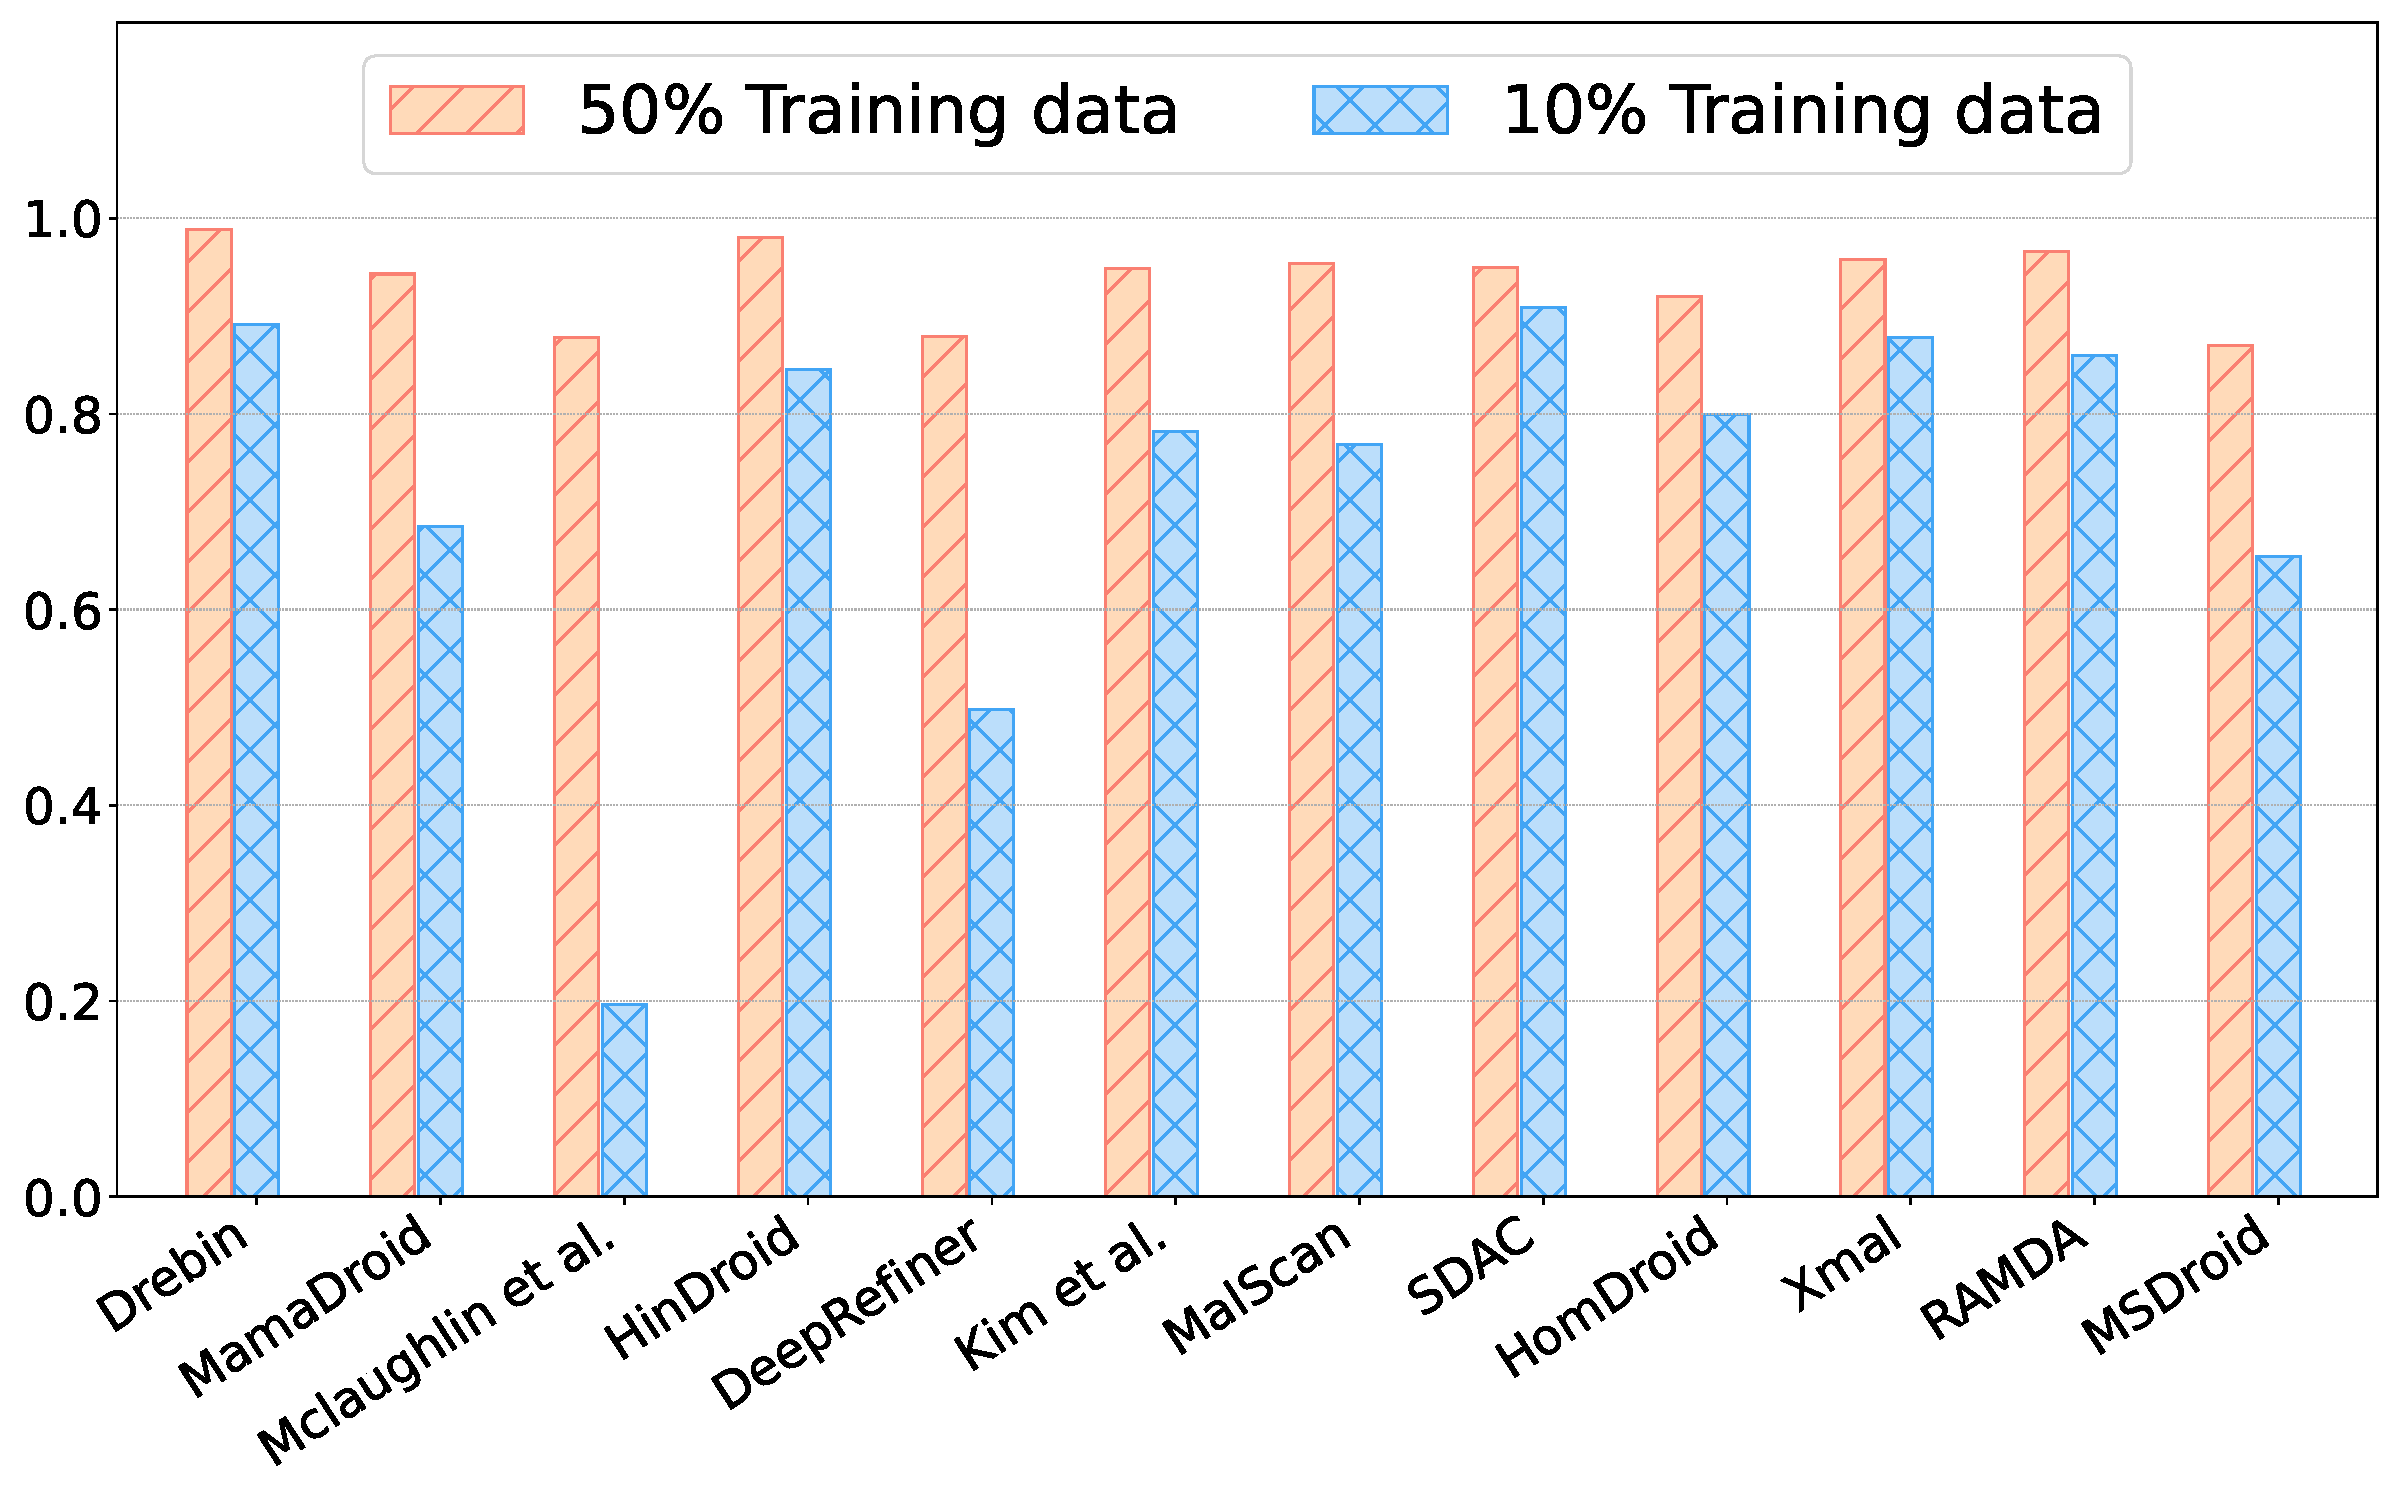
\includegraphics[width=0.64\linewidth]{fig/training_size.pdf}
    \vspace{-0.2cm}
    \caption{Effectiveness of the selected approaches using different sizes of training data.}
    \label{fig:training_size}
    \vspace{-0.5cm}
\end{figure}

% \subsection{Effectiveness vs. Semantics Levels\tdsc{(Domain Semantics?)}}

\bulletpoint{APK feature}
Android malware detectors often leverage diverse features to enhance detection performance~\cite{arp2014drebin,kim2018multimodal,li2021robust}.
The reason is that each feature contributes to characterizing APKs, encoding their unique semantics.
One question arises: does the incorporation of more features necessarily enhance a detector's performance?
To investigate this, we remove individual features from the original feature set to assess the resulting performance.
For this experiment, it is essential that the features of the chosen approaches are decomposable, allowing the sequential removal of individual features.
Accordingly, we spotlight Drebin, Kim et al., Xmal, and RAMDA, owing to their decomposable feature sets.
We exclude methods whose features are highly intertwined.
For instance, MamaDroid and MalScan rely on specific API calls to extract features from program graphs, making it challenging to remove individual features --- if API calls are removed, the graph features will also be removed.

Table~\ref{tab:combination_feats} presents the outcomes of this experiment.
From the table, we observe that Drebin, Xmal, and RAMDA have performance degradation when one feature is removed.
Interestingly, Kim et al. deviate from this trend.
In fact, even after omitting several features, its performance exceeds the original results.
These two observations underscore:
(i) each feature contains unique semantics describing the APKs and contributes to the overall effectiveness of a malware detector, and (ii) the semantics of different feature sets are not always complementary, and merely expanding the feature set does not guarantee enhanced performance.
This phenomenon underscores the importance of evaluating and justifying the inclusion of each feature in a malware detector based on the semantics.

\tosem{Add experiments for Kim, training epoch, and hidden size dimension.}

% These two observations underscore that each feature contributes to the overall effectiveness of a malware detector.
% While in some cases, merely expanding the feature set does not guarantee enhanced performance.

% {\bf This phenomenon underscores the importance of evaluating and justifying the inclusion of each feature in a malware detector based on the semantics.}

\begin{table}[t]
    \centering
    \renewcommand{\arraystretch}{0.8}
    \caption{The impact of APK features on the effectiveness of Drebin, Kim et al., Xmal, and RAMDA.}
    % \vspace{-0.1cm}
    \begin{adjustbox}{width=0.86\linewidth, center}
 \begin{tabular}{@{}l|cc|cc|cc|cc@{}}
 \toprule
 \multirow{2}{*}{\textbf{\raisebox{-0.2cm}{\begin{tabular}[c]{@{}l@{}}Feature\\ Combination\end{tabular}}}} & \multicolumn{2}{c|}{\textbf{Drebin}}      & \multicolumn{2}{c|}{\textbf{Kim et al.}}  & \multicolumn{2}{c|}{\textbf{Xmal}} & \multicolumn{2}{c}{\textbf{RAMDA}} \\ \cmidrule(l){2-9} 
 & \multicolumn{1}{c|}{\textbf{F1}} & \textbf{Acc.} & \multicolumn{1}{c|}{\textbf{F1}} & \textbf{Acc.} & \multicolumn{1}{c|}{\textbf{F1}} & \textbf{Acc.} & \multicolumn{1}{c|}{\textbf{F1}} & \textbf{Acc.} \\ \midrule
 Original   & \multicolumn{1}{c|}{\textbf{0.722}}& \textbf{0.948}  & \multicolumn{1}{c|}{0.726}& 0.944  & \multicolumn{1}{c|}{\textbf{0.698}}& \textbf{0.942}  & \multicolumn{1}{c|}{\textbf{0.636}}& \textbf{0.905}  \\ \midrule
 w/o hardware& \multicolumn{1}{c|}{0.717}& 0.947  & \multicolumn{1}{c|}{0.728}& 0.945  & \multicolumn{1}{c|}{N/A}  & N/A    & \multicolumn{1}{c|}{N/A}  & N/A    \\ \midrule
 w/o app-intent & \multicolumn{1}{c|}{0.622}& 0.936  & \multicolumn{1}{c|}{\textbf{0.776}}& \textbf{0.952}  & \multicolumn{1}{c|}{N/A}  & N/A    & \multicolumn{1}{c|}{0.428}& 0.845  \\ \midrule
 w/o permission & \multicolumn{1}{c|}{0.698}& 0.945  & \multicolumn{1}{c|}{0.692}& 0.939  & \multicolumn{1}{c|}{0.566}& 0.926  & \multicolumn{1}{c|}{0.526}& 0.882  \\ \midrule
 w/o api call& \multicolumn{1}{c|}{0.691}& 0.944  & \multicolumn{1}{c|}{0.699}& 0.942  & \multicolumn{1}{c|}{0.639}& 0.930  & \multicolumn{1}{c|}{0.482}& 0.880  \\ \midrule
 w/o opcode & \multicolumn{1}{c|}{N/A}  & N/A    & \multicolumn{1}{c|}{0.724}& 0.942  & \multicolumn{1}{c|}{N/A}  & N/A    & \multicolumn{1}{c|}{N/A}  & N/A    \\ \midrule
 w/o code string& \multicolumn{1}{c|}{0.702}& 0.944  & \multicolumn{1}{c|}{0.725}& 0.945  & \multicolumn{1}{c|}{N/A}  & N/A    & \multicolumn{1}{c|}{N/A}  & N/A    \\ \bottomrule
 \end{tabular}
    \end{adjustbox}
    \label{tab:combination_feats}
    % \centering
    \begin{tablenotes}[flushleft, labelsep=0]
 \footnotesize
 \item \noindent w/o means without. N/A denotes features are not used in the original work.
 \end{tablenotes}
    \vspace{-0.5cm}
\end{table}


\bulletpoint{Model type}
Given specific features that describe app behaviors, different models can be used to extract semantics and detect malware.
The features reflect the richness of the available semantics, while the models determine how effectively these semantics are leveraged.
In this section, we select MamaDroid, HinDroid, and MalScan, which share the same feature set and feature representation, as shown in Table~\ref{tbl:systematization}, to evaluate the impact of different models on the effectiveness of malware detectors.
From the results in Table~\ref{tab:res_ratio} under scenario \ding{182}, we observe that HinDroid outperforms MamaDroid and MalScan.
This suggests that given a fixed feature set, different models demonstrate varying capabilities in extracting semantics and detecting Android malware.

\bulletpoint{Feature and model combination investigation}
\tosem{choose several models, (RF, SVM, KNN, MLP) and evaluated these models with specifc set of features (Hardware component, application component, intent, permission, API call, opcode, code string, resource information).
Point to there are lots of combination of features, and hint that maybe choose specific features for certain kinds of malware is a trend.
}

\begin{conclusionbox}
    \textit{Summary:}
    The effectiveness of ML-based malware detectors is shaped by various factors, such as APK features and model types. At the core of these influences is the richness of semantics embedded in the features and the models' capability to extract and utilize these semantics.
\end{conclusionbox}



% \vspace{-0.1cm}
\subsection{Robustness against real-world scenarios}
\label{robustness}
Previous works~\cite{pendlebury2019tesseract,li2023black,gao2024comprehensive} have started investigating the resilience of detectors when faced with real-world challenges such as malware evolution, obfuscation, and adversarial attacks.
Nonetheless, they often focus on a subset of these challenges or employ unrealistic experimental settings, potentially skewing their findings.
For instance, \textsc{Tesseract}~\cite{pendlebury2019tesseract} explores the impact of malware evolution, while Gao~\cite{gao2024comprehensive} assesses the robustness of detectors using an unrealistic balanced dataset.
This section aims to fill these gaps by thoroughly re-evaluating the robustness of the selected approaches in real-word settings, providing a clearer picture of where ML-based malware detection stands today.

\begin{figure*}[t]
    \centering
    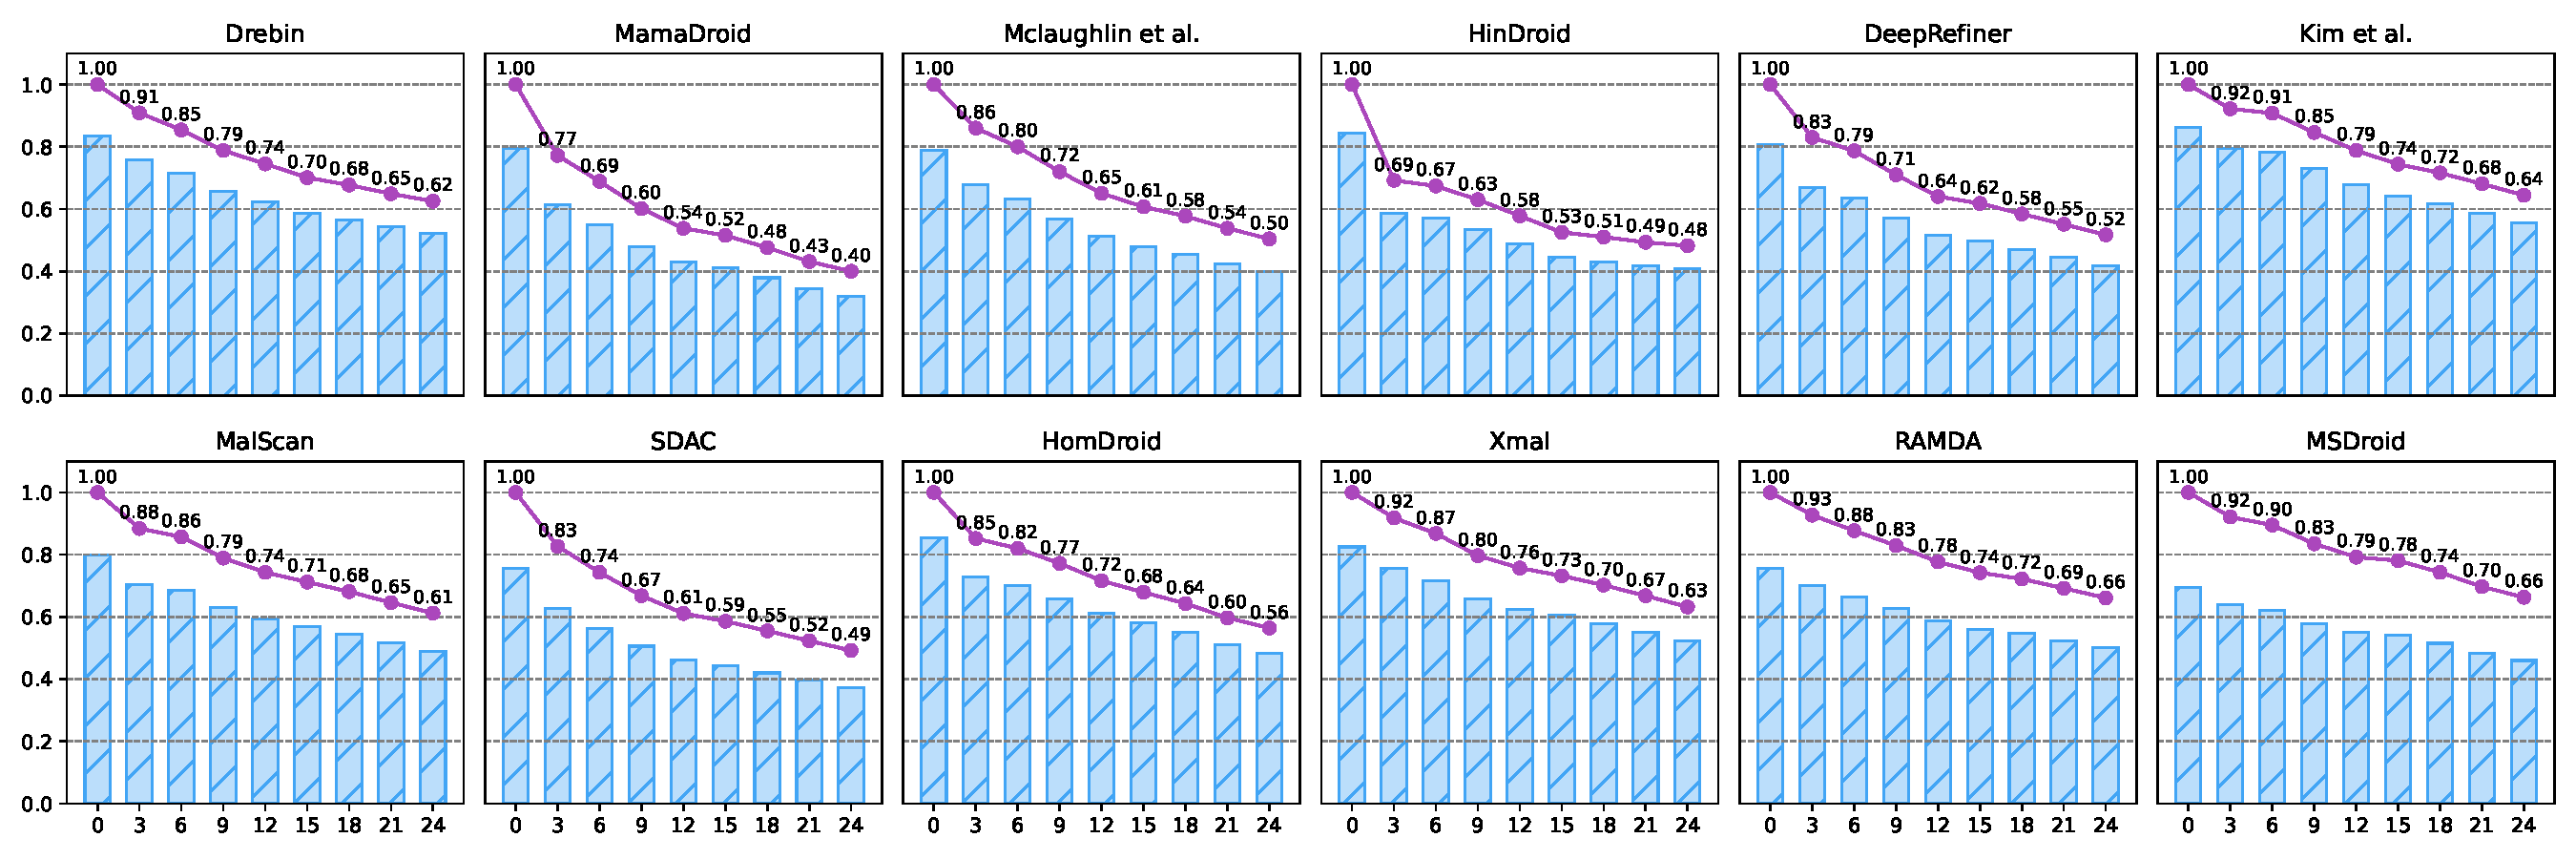
\includegraphics[width=\linewidth]{fig/evolution.pdf}
    % \vspace{-0.1cm}
    \caption{The performance of the selected techniques against diverse malware evolution periods. Columns display the absolute values of $AUT(F1, N)$.
    The line charts depict the relative percentage of $AUT(F1, N)$ against $AUT(F1, 0)$.}
    \label{fig:evolution}
\vspace{-0.3cm}
\end{figure*}

\bulletpoint{Malware evolution}
To quantify the impact of evolution on malware detectors, we utilize the $AUT(f, N)$~\cite{pendlebury2019tesseract}, where $f$ denotes the F1-score of a given approach, and $N$ represents the evolution period. 
The definition of $AUT(f, N)$ can be found in the Appendix~\ref{sub:aut}.
We set $N$ to 3, 6, 9, 12, 15, 18, 21, and 24 months in this experiment.
This metric ranges in (0, 1), where higher values indicate greater resilience to malware evolution.
In the study, we adopt a rolling algorithm over the data from 2011 to 2020 to calculate the $AUT(f, N)$.
Specifically, for each year, from 2011 to 2020, we first partition the data into training, validation, and testing sets with \texttt{8:1:1}.
Next, we train models with the training data, validate to get the best model, and evaluate it on the test set to get the F1-score as $AUT(F1, 0)$.
Then, the model is applied to test data in the next $N$ months, yielding $N$ F1-scores. 
These scores are further used to calculate the $AUT(F1, N)$.
By averaging the $AUT(F1, N)$ values sourced from distinct yearly datasets, we chart the outcomes in Figure~\ref{fig:evolution}.

It is clear that malware evolution affects the effectiveness of these selected techniques.
This is within expectations, as malware evolves over time, the semantics of malware may change, making it harder for detectors to capture these changes.
Most DL approaches display superior resilience against malware evolution compared to their TML counterparts.
Specifically, the majority of DL techniques retain about 60\% effectiveness even after two years. 
In contrast, many TML methods see their F1-scores reduced to 50\% within the same time span.
This disparity can be traced back to the inherent capability of DL methods to discern intricate patterns, which TML might miss.
Interestingly, Mclaughlin et al. and DeepRefiner, do not fare as well over time.
This could be attributed to their reliance on apps' original bytecode as input, which may contain more noise and complicate the semantic extraction process.
\tosem{Add more analysis how to improve the robustness}

\begin{table}[t]
    \centering
    \renewcommand{\arraystretch}{0.7}
    \caption{The F-score of the selected approaches under different obfuscation strategies~\cite{aonzo2020obfuscapk}.}
    % \vspace{-0.1cm}
    \begin{adjustbox}{width=0.74\linewidth, center}
    \begin{tabular}{@{}c|c|c|c|c|c@{}}
    \toprule
    \diagbox[innerleftsep=-0.1em, innerrightsep=-0.3em, height=2.7em,width=7em]{\textbf{Approach}}{\textbf{Obfuscation}} & \textbf{\begin{tabular}[c]{@{}c@{}}Without \\ Obfus.\end{tabular}} & \textbf{\begin{tabular}[c]{@{}c@{}}Rename \\ Identifier\end{tabular}} & \textbf{\begin{tabular}[c]{@{}c@{}}Encrypt \\ Resource\end{tabular}} & \textbf{\begin{tabular}[c]{@{}c@{}}Modify \\ Code\end{tabular}} & \textbf{\begin{tabular}[c]{@{}c@{}}Reflect \\ Invocation\end{tabular}} \\ \midrule
    Drebin      & 0.732 & 0.702 & 0.701 & 0.732 & 0.732 \\ \midrule
    MamaDroid   & 0.653 & 0.274 & 0.449 & 0.150 & 0.461 \\ \midrule
    Mclaughlin et al.  & 0.750 & 0.699 & 0.722 & 0.175 & 0.727 \\ \midrule
    HinDroid    & 0.750 & 0.750 & 0.741 & 0.750 & 0.735 \\ \midrule
    DeepRefiner & 0.692 & 0.618 & 0.658 & 0.297 & 0.612 \\ \midrule
    Kim et al.  & 0.795 & 0.795 & 0.611 & 0.795 & 0.798 \\ \midrule
    MalScan     & 0.675 & 0.675 & 0.675 & 0.681 & 0.687 \\ \midrule
    SDAC & 0.563 & 0.538 & 0.552 & 0.495 & 0.552 \\ \midrule
    HomDroid    & 0.729 & 0.751 & 0.706 & 0.728 & 0.739 \\ \midrule
    Xmal & 0.727 & 0.727 & 0.727 & 0.727 & 0.727 \\ \midrule
    RAMDA& 0.635 & 0.635 & 0.635 & 0.635 & 0.635 \\ \midrule
    MSDroid     & 0.672 & 0.675 & 0.610 & 0.356 & 0.494 \\ \bottomrule
    \end{tabular}
    \end{adjustbox}
    \label{table:res_obfuscation}
    \vspace{-0.3cm}
\end{table}

\bulletpoint{Obfuscation}
Obfuscation techniques often alter an app's code. 
It can also affect the effectiveness of malware detectors~\cite{he2022msdroid}.
This part explores the influences of popular obfuscation techniques, \textit{i.e.,} renaming identifiers, encrypting resources, modifying code, and invoking reflection~\cite{aonzo2020obfuscapk}, on the selected approaches.

We apply the obfuscation strategies discussed earlier to the testing set in Table~\ref{tab:effectiveness_dataset}(\ding{182}).
Only the apps that can be successfully obfuscated by all the strategies are included in the obfuscated testing set, which contains 1,303 apps.
The effectiveness of the selected approaches, previously trained on the original training set, is then evaluated on this obfuscated testing set.
Table~\ref{table:res_obfuscation} summarizes the results.
Clearly, most methods exhibit a performance decrease when subjected to obfuscation.
This is expected, as obfuscation can hidden the malicious semantics, making it harder for detectors to capture them.
Specifically, the impact of obfuscation on detectors significantly depends on how the detectors utilize APK features.
For instance, Xmal and RAMDA show greater robustness against obfuscation.
This is mainly because the employed obfuscation techniques do not change their used features.
In contrast, MamaDroid and MSDroid, relying on the code structure, tend to be more susceptible to the code modification.
This suggests that the impact of obfuscation on detectors is closely related to the degree to which obfuscation techniques alter the semantics of the features utilized by the detectors.
Also, by comparing MamaDroid and MSDroid --- both relying on the code structure --- we observe that a detector's robustness against obfuscation is also shaped by the model's semantic extraction capability.
\tosem{- permission from manifest
- extracted APIs, the list is hardcode, we simiply check the obfuscation, system api, doest not check it.
}


\bulletpoint{Adversarial attack}
We now utilize the dataset from Table~\ref{tab:effectiveness_dataset}(\ding{182}) to explore the impact of adversarial attacks on the performance of these selected approaches.
It is worth noting that we exclude approaches Mclaughlin et al. and DeepRefiner from this experiment.
This is because they truncate features at a certain size, making them easily bypassable.
Attackers can embed malicious code in the ignored part to evade detection.


% Mclaughlin et al. and DeepRefiner are excluded since they truncate features at a certain size, making them easily bypassable.
% Attackers can embed malicious code in the ignored part to evade detection.

To investigate the impact of adversarial attacks, we employ two primary strategies: Jacobian Saliency Map Attack (JSMA) and Randomized Input (RI).
These two techniques are chosen for their simplicity and effectiveness, compromising most ML-based malware detectors, as shown in Table~\ref{tab:adversarial}.
This suggests that more advanced attack strategies could pose even greater threats to these detectors~\cite{he2023efficient,zhao2021structural}.
For JSMA, we first train a substitute model with the training set, followed by applying JSMA to the model to generate adversarial samples.
For RI, we randomly change a certain percentage of features in the testing set to produce adversarial examples.
When crafting adversarial samples, we follow~\cite{li2023black,chen2019android} to ensure the feature modifications are domain-mappable and can be repackaged to APKs.
For feature-vector-based approaches like Drebin, we follow~\cite{chen2019android} by constraining modifications to vector bits that are 0, changing them to 1.
This ensures that all required permissions and functions remain unchanged, keeping the app's functionality unaffected.
For graph-based solutions, we introduce non-disruptive modifications to the graph structures that do not alter the app's functionality.
The graph structure includes non-leaf nodes (user-defined functions) and leaf nodes (Android API). 
When adding a new edge, we select a non-leaf node in the graph and add a try block with a callee chosen from leaf nodes.
Since leaf nodes do not call any other nodes, the added edge does not affect the app's functionality.
% Taking Drebin as an example, we restrict our modifications to changing feature vectors from 0 to 1, keeping apps' functionalities unaffected.
To measure the robustness against adversarial attacks, we use two metrics from~\cite{li2023black}: Adversarial Success Rate (ASR) and Adversarial Perturbation Ratio (APR).
The detailed definitions can be found in the Appendix~\ref{sub:aut}.
Both metrics range (0, 1).
A higher ASR indicates increased vulnerability to adversarial attacks, while a higher APR suggests greater robustness against such attacks due to the model's ability to withstand perturbations.

By analyzing Table~\ref{tab:adversarial}, we note that JSMA yields an average ASR of 98.8\% across the evaluated approaches, indicating their vulnerability to such basic adversarial attacks, let alone more sophisticated ones~\cite{he2023efficient}.
The employed strategies are less effective on MamaDroid, HomDroid, and RAMDA.
The reason for MamaDroid and HomDroid could be linked to their abstraction of APKs' graph structures.
Interestingly, MamaDroid, HomDroid, and MalScan all utilize API calls and program graphs; the former two methods demonstrate greater resilience.
The key difference lies in their handling of program graphs --- MamaDroid abstracts these graphs using family and package names, and HomDroid employs social network triads for abstraction, in contrast to MalScan's direct use of the graphs.
These abstractions make the malicious semantics encoded in graph structures more resistant to perturbation, enhancing the robustness of the detectors built on them.
Additionally, RAMDA's resilience can be attributed to its customized Autoencoder, which learns compressed representations of benign apps, making it more defensive to adversarial examples.
These findings suggest that abstracting feature representations or augmenting models' defensive capabilities could improve malware detectors' robustness to adversarial attacks.

\begin{table}[t]
    \renewcommand{\arraystretch}{0.73}
    \caption{The robustness of our selected approaches on various adversarial attacks.}
    % \vspace{-0.1cm}
    \begin{adjustbox}{width=0.7\linewidth, center}
 \begin{tabular}{@{}c|cc|c||c|cc|c@{}}
  \toprule
  \multirow{2}{*}{\textbf{\begin{tabular}[c]{@{}c@{}}Selected\\ Approach\end{tabular}}} & \multicolumn{2}{c|}{\textbf{ASR}}      & \multirow{2}{*}{\textbf{APR}} & \multirow{2}{*}{\textbf{\begin{tabular}[c]{@{}c@{}}Selected\\ Approach\end{tabular}}} & \multicolumn{2}{c|}{\textbf{ASR}}      & \multirow{2}{*}{\textbf{APR}} \\ \cmidrule(lr){2-3} \cmidrule(lr){6-7}
   & \multicolumn{1}{c|}{\textbf{JSMA}} & \textbf{RI} &    &  & \multicolumn{1}{c|}{\textbf{JSMA}} & \textbf{RI} &    \\ \midrule
  Drebin  & \multicolumn{1}{c|}{1.000}  & 0.237& 0.001 & SDAC    & \multicolumn{1}{c|}{1.000}  & 0.146& 0.001 \\ \midrule
  MamaDroid  & \multicolumn{1}{c|}{0.972}  & 0.187& 0.021 & HomDroid& \multicolumn{1}{c|}{0.979}  & 0.303& 0.324 \\ \midrule
  HinDroid& \multicolumn{1}{c|}{1.000}  & 0.068& 0.004 & Xmal    & \multicolumn{1}{c|}{1.000}  & 0.142& 0.013 \\ \midrule
  Kim et al.  & \multicolumn{1}{c|}{1.000}  & 0.000& 0.004 & RAMDA   & \multicolumn{1}{c|}{0.931}  & 0.300& 0.023 \\ \midrule
  MalScan & \multicolumn{1}{c|}{1.000}  & 0.788& 0.001 & MSDroid & \multicolumn{1}{c|}{1.000}  & 0.022& 0.013 \\ \bottomrule
  \end{tabular}
    \end{adjustbox}
    \label{tab:adversarial}
\vspace{-0.3cm}
\end{table}

\begin{conclusionbox}
    \textit{Summary:}
    ML-based malware detectors are susceptible to various real-world challenges, including malware evolution, obfuscation, and adversarial attacks. \textit{Malware semantics} play a crucial role in determining the robustness of detectors against these challenges.
\end{conclusionbox}



% \vspace{-0.1cm}
\subsection{Efficiency}
\label{efficiency}
In this section, we scrutinize the efficiency of the selected methods across datasets from different years, focusing on both feature transformation and ML modeling.
For fairness, we normalize the time taken by these methods based on the analysis of 20,000 apps per year.
All experiments are performed on a server with 32-core CPUs operating at 2.10 GHz, 251 GB of physical memory, and two GPUs, each with 32 GB of memory.

\bulletpoint{Feature transformation}
With the pre-extracted features, we assess the time efficiency of the selected methods in retrieving and encoding their required features.
Note that we utilize 16 processes to transform the features concurrently.

Figure~\ref{fig:efficiency_encoding} depicts the time taken by these approaches for feature transformation.
As time advances, a noticeable increase in the time required for processing is evident, which aligns with the exponential growth in the size and complexity of APKs over the years.
This observation underscores the importance of designing efficient feature extraction strategies to keep pace with the rapid evolution of Android applications.
Notably, there is a significant variance in the time consumption among different approaches.
This is within our expectation since various methods employ distinct features and encoding techniques.
For instance, SDAC consumes the most time due to its requirement to query the program graph recursively for API call sequence generation.
While methods like Xmal and RAMDA are more time-efficient, as they perform a one-time traversal on the program graph to capture API calls.

\bulletpoint{ML modeling}
For each yearly dataset, we divide it into training, validation, and testing sets with a ratio of \texttt{8:1:1}.
We then calculate the time required by the selected methods for model training and testing.
Note that we take the early stopping strategy during the training phase for DL models.

Table~\ref{tab:efficiency_ml_modeling} details the training time taken by these approaches. 
From a horizontal perspective, we observe that most DL techniques require more time than their TML counterparts. 
Furthermore, model complexity directly correlates with its training duration. 
Analyzing longitudinally, there is a clear trend: as years progress, the time requirements for these methods increase. 
This can be attributed to apps growing in complexity and an expanding feature set.
When combined with the effectiveness (Sec.~\ref{effectiveness}), we note that detection effectiveness does not always match resource utilization.
Striking a balance between effectiveness and efficiency is critical when developing new detectors, where semantics plays a key role in deciding the balance.



\begin{figure}[t]
    \centering
    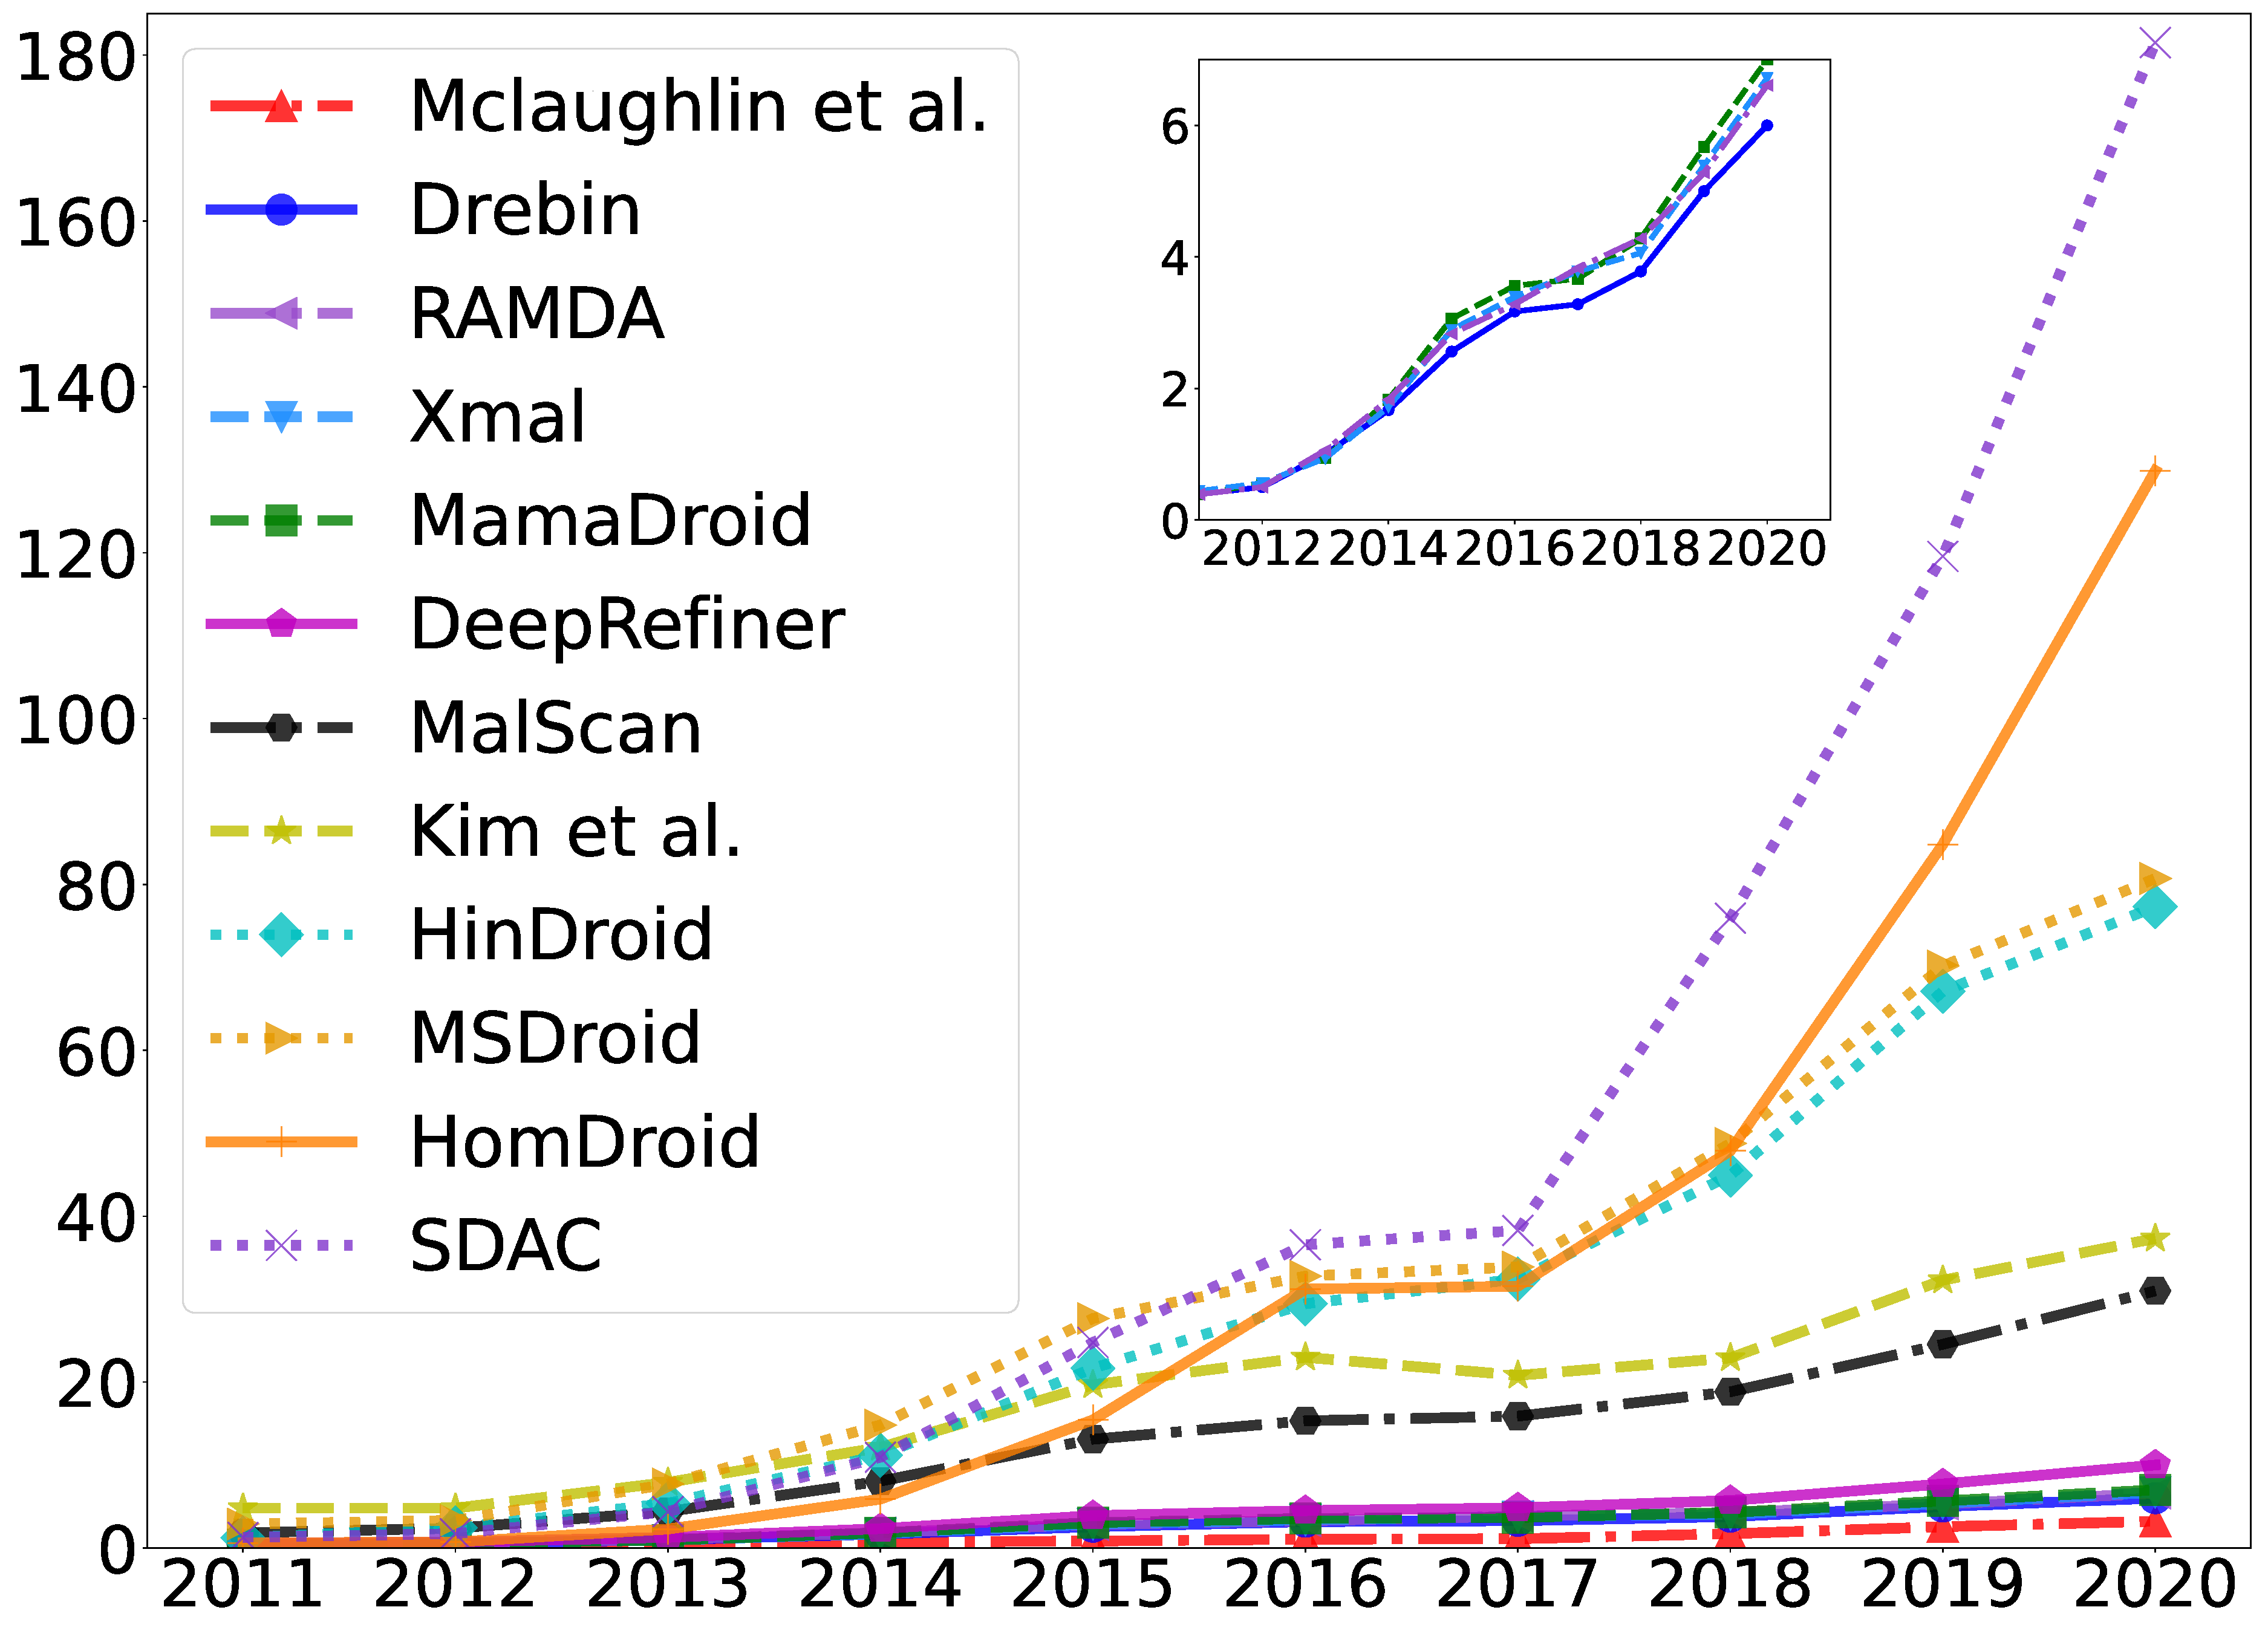
\includegraphics[width=0.56\linewidth]{fig/efficiency_encoding.pdf}
    % \vspace{-0.2cm}
    \caption{The efficiency of feature transformation of the selected approaches. The x-axis shows the dataset year, and the y-axis indicates the utilized time in hours.}
    \label{fig:efficiency_encoding}
    \vspace{-0.3cm}
\end{figure}

\begin{conclusionbox}
    \textit{Summary:}
    The efficiency of ML-based malware detectors does not positively correlated with their effectiveness. Finding a balance between these two aspects is crucial when developing new detectors, requiring careful alignment of feature semantics with model capabilities to achieve an optimal trade-off.
\end{conclusionbox}

\subsection{Further Experimental Validation}
\label{further_experiments}

\subsubsection{\textbf{Influence of Reverse Engineering Tools}}
\label{tool_influence}

\tosem{use APK tool to handle maybe 4000 apps, and then extract specific features, to test the influence of features for specific models (such as MLP, RF, SVM,...)
with new experiments dataset.}

\subsubsection{\textbf{Detection Effectiveness}}
\label{sec:detect_effectiveness}

\tosem{add the experiments year by year, to say the result is stable.
add 21-24 data, and re-run some experiments (effectiveness, evolution)}

\subsubsection{\textbf{Detection Efficiency}}
\label{sec:detect_efficiency}

\tosem{discuss the efficiency metrics, and add new efficiency metrics, and add new experiments}
% \vspace{-0.1cm}
\section{Findings and Recommendations}
\label{sec:findings}
We now draw from our findings to discuss the current state of ML-based Android malware detection and put forth recommendations to guide future research in this area.

% \subsection{Findings}
% \label{sec:findings}
\bulletpoint{Findings}
We summarize our key findings as follows:

\noindent \textit{(1) Current ML-based Android malware detectors still face open challenges.}
While ML models have been evidently effective in detecting malware~\cite{he2022msdroid,kim2018multimodal,li2021robust,mariconti2016mamadroid}, their effectiveness is still far from satisfactory when faced with challenging scenarios such as limited data size, rapid malware evolution, and adversarial attacks.

\noindent \textit{(2) Selecting features relevant to malware semantics is crucial for effective detection.}
A wide range of APK features, such as permissions and intents, have been leveraged for malware detection~\cite{xu2018deeprefiner,arp2014drebin,kim2018multimodal}.
These features serve to profile app behavior and play a critical role in determining detector effectiveness.
Our findings suggest that heuristic feature selection can effectively reduce noise in the feature space, allowing models to more readily identify malicious patterns --- particularly in data-scarce settings.
However, we also observe that the semantics captured by different feature types are not always complementary, and principled strategies for combining them remain underexplored.
Consequently, naively incorporating additional features does not necessarily yield improved detection performance.

% Our analysis reveals that feature engineering helps models to discern malicious patterns when data is limited.
% However, including more features randomly does not guarantee enhanced performance. 
% Thus, researchers should carefully select features to improve the effectiveness and efficiency.
\noindent \textit{(3) More complex models are not a silver bullet in designing malware detectors.}
The literature reflects the trend towards employing more powerful ML models to detect malware~\cite{xu2018deeprefiner,arp2014drebin}.
Our analysis reveals that DL-based methods appear to be more resilient than TML-based approaches in adapting to malware evolution.
However, we also find that DL-based approaches are less effective than TML-based methods when the malware-to-goodware ratio is low.
This suggests that utilizing more complex models is not a universal solution for malware detection.
Instead, the choice of models should take into account the richness of the semantic information derived from the features.
One more practical observation is given feature sets including discrete features (\textit{i.e.,} permissions and API calls), ensembling models and DL models with embedding layers tend to outperform other typical models.


% When introducing a new model to detect malware, it is crucial to justify the rationale behind it.

\noindent \textit{(4) Both feature abstraction and models' defensive mechanism contribute to detectors' robustness.}
Our analysis indicates that abstracting features can help models capture robust malicious patterns~\cite{bhagoji2018enhancing}.
For instance, MamaDroid~\cite{mariconti2016mamadroid} abstracts program graphs with families and packages, enhancing its robustness to adversarial attacks.
Moreover, bolstering the defensive capability of ML models can further amplify detectors' reliability and stability~\cite{papernot2016distillation}.

\noindent \textit{(5) Detection effectiveness does not positively correlate with efficiency.}
Through a combined analysis of effectiveness and efficiency, we observe that effectiveness and efficiency do not always positively correlate.
A detector demanding more resources does not necessarily deliver enhanced results.
For example, Drebin~\cite{arp2014drebin} can achieve competitive detection performance with relatively low resource consumption.


% \begin{table*}[t]
%     \centering
%     \renewcommand{\arraystretch}{1.15}
%     \caption{The efficiency (\textit{i.e.,} model training time) of selected approaches across datasets from different years.}
%     % \vspace{-0.1cm}
%     \begin{adjustbox}{width=\textwidth}
%         \begin{tabular}{@{}r|r|r|r|r|r|r|r|r|r|r|r|r@{}}
%             \toprule
%             \textbf{Year} & \multicolumn{1}{c|}{\textbf{Drebin}} & \multicolumn{1}{c|}{\textbf{MamaDroid}} & \multicolumn{1}{c|}{\textbf{Mclaughlin}} & \multicolumn{1}{c|}{\textbf{HinDroid}} & \multicolumn{1}{c|}{\textbf{DeepRefiner}} & \multicolumn{1}{c|}{\textbf{Kim}} & \multicolumn{1}{c|}{\textbf{MalScan}} & \multicolumn{1}{c|}{\textbf{SDAC}} & \multicolumn{1}{c|}{\textbf{HomDroid}} & \multicolumn{1}{c|}{\textbf{Xmal}} & \multicolumn{1}{c|}{\textbf{RAMDA}} & \multicolumn{1}{c}{\textbf{MSDroid}} \\ \midrule
%             \textbf{2011} & 15.11s        & 1.90s            & 128m22s                  & 2m19s           & 369m18s            & 98m47s            & 1m14s          & 84m47s      & 2.00s           & 1m15s       & 1m6s         & 20m19s        \\ \midrule
%             \textbf{2012} & 20.88s        & 1.94s            & 97m01s                   & 2m18s           & 359m35s            & 92m47s            & 1m18s          & 89m05s      & 2.04s           & 1m25s       & 1m11s        & 37m54s        \\ \midrule
%             \textbf{2013} & 22.37s        & 2.12s            & 172m20s                  & 2m13s           & 477m18s            & 115m40s           & 1m24s          & 115m35s     & 2.04s           & 50.36s      & 1m06s        & 40m11s        \\ \midrule
%             \textbf{2014} & 32.49s        & 2.46s            & 128m13s                  & 2m40s           & 629m26s            & 104m03s           & 1m33s          & 132m55s     & 2.20s           & 2m20s       & 1m17s        & 42m07s        \\ \midrule
%             \textbf{2015} & 26.40s        & 2.60s            & 411m03s                  & 2m44s           & 730m41s            & 115m27s           & 1m38s          & 250m07s     & 2.22s           & 2m10s       & 1m20s        & 42m52s        \\ \midrule
%             \textbf{2016} & 32.62s        & 2.99s            & 234m19s                  & 2m51s           & 867m25s            & 135m50s           & 1m42s          & 470m38s     & 2.26s           & 1m05s       & 1m19s        & 142m23s       \\ \midrule
%             \textbf{2017} & 22.36s        & 2.75s            & 192m41s                  & 2m28s           & 997m04s            & 145m24s           & 1m37s          & 296m05s     & 2.22s           & 1m54s       & 1m20s        & 47m22s        \\ \midrule
%             \textbf{2018} & 19.97s        & 2.91s            & 227m48s                  & 2m36s           & 933m12s            & 128m32s           & 1m34s          & 716m43s     & 2.21s           & 1m19s       & 1m21s        & 155m50s       \\ \midrule
%             \textbf{2019} & 26.83s        & 3.03s            & 514m18s                  & 2m34s           & 968m50s            & 185m43s           & 1m32s          & 918m09s     & 2.22s           & 1m34s       & 1m18s        & 130m41s       \\ \midrule
%             \textbf{2020} & 22.87s        & 2.69s            & 771m44s                  & 2m22s           & 1064m30s           & 148m08s           & 1m29s          & 867m55s     & 2.17s           & 2m09s       & 1m12s        & 93m08s        \\ \bottomrule
%             \end{tabular}
%     \end{adjustbox}
%     \label{tab:efficiency_ml_modeling}
% \vspace{-0.5cm}
% \end{table*}

\bulletpoint{Recommendations}
Our findings reveal that the effectiveness of ML-based Android malware detectors is closely tied to the quantity and quality of malware semantics extracted from APK features, which describe the malicious behaviors of apps.
To design more effective and robust detectors, we recommend the following strategies:

\noindent \textit{(1) Quantify malware semantics.}
Instead of simply incorporating more features to enhance detection performance, one can design metrics to evaluate the quantity and quality of malware semantics captured by the features, as well as the redundancy among them.
This can guide researchers in selecting features that are more informative and complementary, improving the effectiveness of detectors.

\noindent \textit{(2) Investigate feature combination and abstraction.}
Given the diverse features available to describe app behaviors, a promising research direction is to explore effective strategies for combining these features to amplify their collective ability to capture malware semantics. 
Additionally, feature abstraction has demonstrated potential in enhancing the robustness of detectors. 
Future work could focus on developing techniques to abstract features in ways that improve detectors' resilience to real-world challenges while maintaining or even enhancing detection performance.

\noindent \textit{(3) Mine invariant malware semantics.}
Noticeable challenges in ML-based Android malware detection include the instability against malware evolution and susceptibility to adversarial attacks.
To address these challenges, researchers can explore invariant malware semantics that remain consistent across different versions of malware.

\noindent \textit{(4) Align model complexity with malware semantics.}
Once the features and their role in describing malware semantics are determined, the next step is selecting models that can effectively utilize this information.
Researchers should carefully match the complexity of the models to the richness of the malware semantics to achieve optimal detection performance.
Failing to do so may result in unnecessary computational overhead without improving detection effectiveness.


% \bulletpoint{Detection effectiveness does not positively correlate with efficiency}
% Through a combined analysis of effectiveness and efficiency, we observe that effectiveness and efficiency do not always positively correlate.
% A detector demanding more resources does not necessarily deliver enhanced results.
% For example, Drebin~\cite{arp2014drebin} can achieve competitive detection performance with relatively low resource consumption.

% \bulletpoint{Current ML-based Android malware detectors still face open challenges}
% While ML models have been evidently effective in detecting malware~\cite{he2022msdroid,kim2018multimodal,li2021robust,mariconti2016mamadroid}, their effectiveness is still far from satisfactory when faced with challenging scenarios such as limited data size, rapid malware evolution, and adversarial attacks.
% Given this context, the field presents substantial opportunities for improvement, particularly in designing robust and practical detectors for real-world usage.


% \subsection*{other findings} 
% performance.
% \vspace{-0.2cm}
\section{Discussion}
\label{sec:discussion}

\begin{figure}[t]
    \centering
    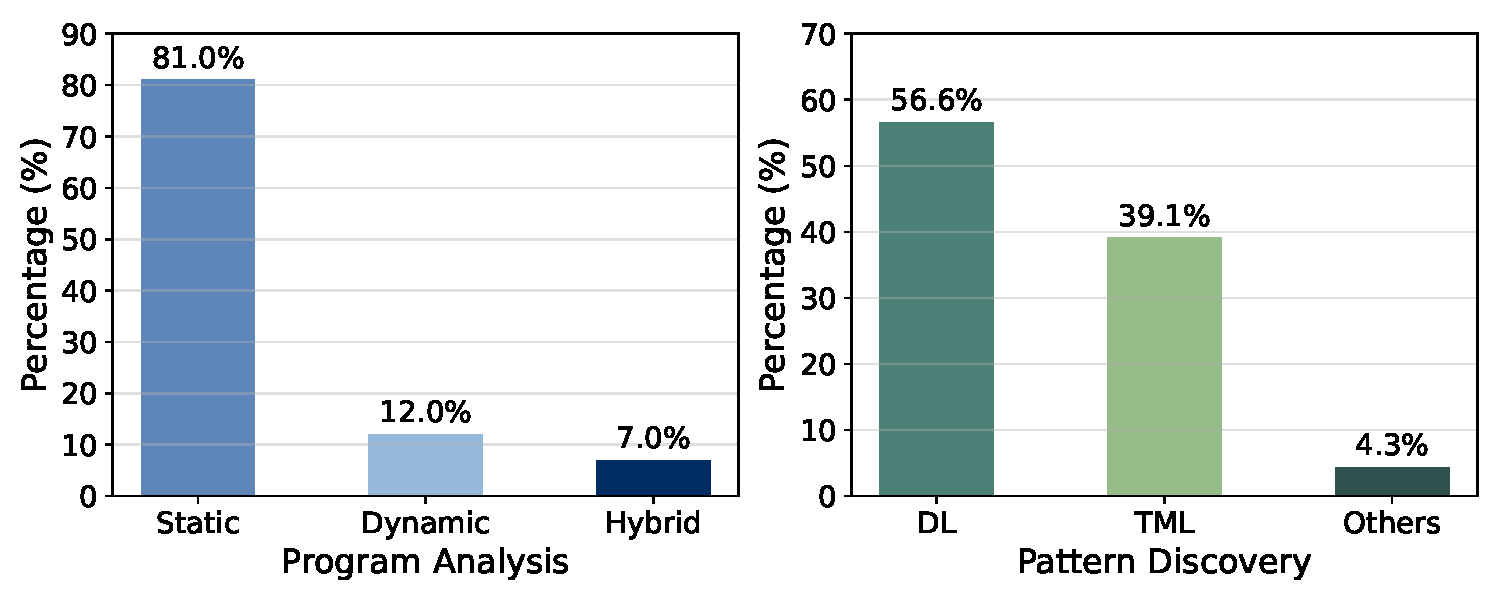
\includegraphics[width=0.76\linewidth]{fig/paper_tech.pdf}
    % \vspace{-0.1cm}
    \caption{The overall distribution of investigated approaches in Android malware detection.}
    \label{fig:paper_distribution}
    \vspace{-0.3cm}
\end{figure}

\bulletpoint{Systematic investigation}
To better understand the efforts dedicated to Android malware detection, we conduct a systematic literature review since 2011.
Aiming for the inclusion of a broad range of papers, we follow the search strategies used in~\cite{liu2022deep,liu2020review}.
Specifically, we perform searches in key digital libraries, such as the ACM Digital Library and IEEE Xplore, using specific keywords, including \texttt{android malware detection}, \texttt{android analysis}, and \texttt{android malware}.
Then, a careful screening of titles and introductions is followed to selectively exclude studies unrelated to our research topic.
This meticulous process ultimately leads to the identification of 258 related papers.

We subsequently categorize these papers based on the program analysis and pattern discovery techniques they employ.
Figure~\ref{fig:paper_distribution} shows the distribution of these techniques.
Our analysis reveals that \textit{static analysis} is the predominant technique utilized to extract features from apps, followed by \textit{dynamic} and \textit{hybrid analysis}.
For pattern discovery, \textit{machine learning}, including both traditional machine learning (TML) and deep learning (DL) models, are extensively used to identify malicious patterns.
Particularly notable is the significant increase in the utilization of static feature extraction and ML-based techniques in recent years. 
This evolving trend highlights the importance of our study, seeking to provide an in-depth understanding of the contemporary landscape in ML-based Android malware detection.

\bulletpoint{Dataset considerations}

\bulletpoint{App packing and it impact}
To protect applications from reverse engineering and tampering, many developers employ app packing techniques that obfuscate the original code structure~\cite{dong2022did,duan2018things}.
Such techniques can substantially degrade the effectiveness of static analysis-based malware detectors, as they hinder the extraction of meaningful features from packed apps.
In this study, to systematically examine the state of ML-based Android malware detection, we focus primarily on unpacked apps, which is consistent with the scope of most prior work~\cite{chen2023continuous,wu2021homdroid}.
During dataset construction, we identify an app as packed if it employs any known packing tools (\textit{e.g.,} Qihoo 360) and exclude these apps to ensure reliable static feature extraction.
We acknowledge that packing techniques can increase static feature extraction failure rates, negatively impacting the performance of static analysis-based detectors.
To mitigate this limitation in practical deployments, future detectors may benefit from integrating static and dynamic analysis techniques, enabling more robust feature extraction in the presence of packing and obfuscation.
In this work, our objective is to evaluate and understand the performance characteristics of ML-based Android malware detectors under controlled and comparable conditions.
A systematic investigation of app packing techniques and their impact on malware detection effectiveness is an important and complementary direction, which we leave for future work.

\bulletpoint{Potential of large language models in Android malware analysis}
Large Language Models (LLMs) have demonstrated remarkable capabilities in natural language processing, code understanding, and reasoning tasks.
Building upon the findings and insights from our study, we believe that LLMs hold substantial promise in the domain of Android malware analysis, particularly in the following areas:
(1) Feature space exploration: LLMs can assist in selecting and combining discriminative features to enhance the performance of malware detectors.
By analyzing the impact of different feature sets on app behavior description, LLMs can guide the construction of more effective and concise feature representations.
(2) Semantic understanding of malicious behavior: LLMs can mine high-level malicious semantics directly from code, improving the interpretability of detection systems and offering deeper insight into the behavioral mechanisms of malware.

For example, LLMs can be employed to analyze various features that describe the same malicious behavior, assess their respective impacts on detector performance, and identify the most effective feature combinations for comprehensive behavior representation.
Furthermore, LLMs can summarize the semantics of a group of functions within an application to uncover specific operations—such as sensitive information collection, data exfiltration, or command-and-control communication.
These semantic summaries can then be used to enhance the characterization and detection of potentially malicious behaviors.

\bulletpoint{Threats to validity}
\jh{There are two main threats to the validity of our study.}
First, our research mainly focuses on investigating general ML-based Android malware detectors.
That is, we do not include the methods designed to solve a particular challenge like malware evolution.
Specifically, there have been several attempts~\cite{narayanan2016adaptive,zhang2020enhancing,chen2023continuous,xu2019droidevolver} starting to mitigate the challenges we have identified.
For instance, the recent APIGraph~\cite{zhang2020enhancing} identifies semantically similar API calls to enhance detectors' robustness against malware evolution.
Integrating this strategy with popular detectors like Drebin and MamaDroid leads to 5\% - 10\% detection improvements over a one-year malware evolution.
Nevertheless, our findings still hold, as these improvements are insufficient compared to the reduction of around 30\% observed in our study.
It is our aspiration that this study can motivate more researchers to focus on these challenges and develop effective solutions to mitigate them.

Second, inconsistencies might exist between our evaluation and the reported ones due to different settings, such as datasets, metrics, and toolchains.
To mitigate experimental biases and provide a fair comparison, we design a general-purpose framework.
Specifically, we adopt standardized techniques across all tasks, including feature extraction and ML modeling.
We also incorporate many evaluation scenarios, such as training data sizes, malware evolution, and efficiency, to ensure a comprehensive measurement using our crafted dataset.
It is our hope that the framework can facilitate future work in ML-based Android malware detection.

\tosem{Disucss the dataset limitation again, and highlgiht our additional experiments again... to say our finding still hold.}
% \vspace{-0.2cm}
\section{Conclusion}
\label{sec:conclusion}
This paper performs the most extensive systematic study of the ML-based Android malware detection literature with empirical and quantitative analysis.
We identify challenges (\textit{i.e.,} unfair comparisons, unrealistic evaluations, and unclear computational costs) that hinder the systematization in this field.
In response, we design a general-purpose framework for developing ML-based detection approaches and evaluating their effectiveness, robustness, and efficiency.
By experimentally comparing 12 representative approaches, our study paints a holistic view of the state of ML-based Android malware detection and puts forth recommendations to guide future research.
For instance, we find existing detectors are still vulnerable to malware evolution and adversarial attacks and in future work, we should focus on incorporating more \textit{malware semantics} to design more practical detectors.
% Committed to the research community's growth, all the artifacts (code, data, and logs) are available at \url{https://anonymous.4open.science/r/RkRyb2lk}.
% Committed to the research community's growth, all the artifacts (code, data, and logs) will be released upon acceptance.

\section*{Acknowledgments}
We thank Bonan Ruan, Jiawei Li, and Chuqi Zhang for their assistance and the anonymous reviewers for their valuable comments.
This research is supported by the National Research Foundation, Singapore, through the National Cybersecurity R\&D Lab at the National University of Singapore under its National Cybersecurity R\&D Programme (Award No. NCR25-NCL P3-0001). 
Any opinions, findings and conclusions or recommendations expressed in this material are those of the authors(s) and do not reflect the views of National Research Foundation, Singapore.


\clearpage
% \balance
\bibliographystyle{ACM-Reference-Format}
\bibliography{paper}
\clearpage
\appendix
\section{Appendix}
This section contains additional data and information that can be of interest to the readers but that are not strictly necessary for understanding the main text.

% \subsection{Publication Statistics Overview}
% \label{sub:publication_statistics}

% We conduct a thorough review of literature spanning from 2011 to 2023 to explore prevalent techniques (\textit{i.e.,} program analysis and patten discovery) in Android malware detection.
% Here, program analysis refers to the methods used to extract features from APK files, while pattern discovery involves the strategies employed to discern patterns from these features.

% To capture as many relevant studies as possible, we take search strategies used in~\cite{liu2022deep,liu2020review}. 
% Our literature search spanned major digital libraries, such as the ACM Digital Library and IEEE Xplore. 
% Throughout the search process, we mainly employ specific keywords to pinpoint relevant papers, including \texttt{android malware detection}, \texttt{android analysis}, and \texttt{android malware}.
% A further manual review of titles and abstracts allows us to filter out papers unrelated to our topic.
% Ultimately, this process yields 258 related papers.

% \begin{figure}[h]
%     \centering
%     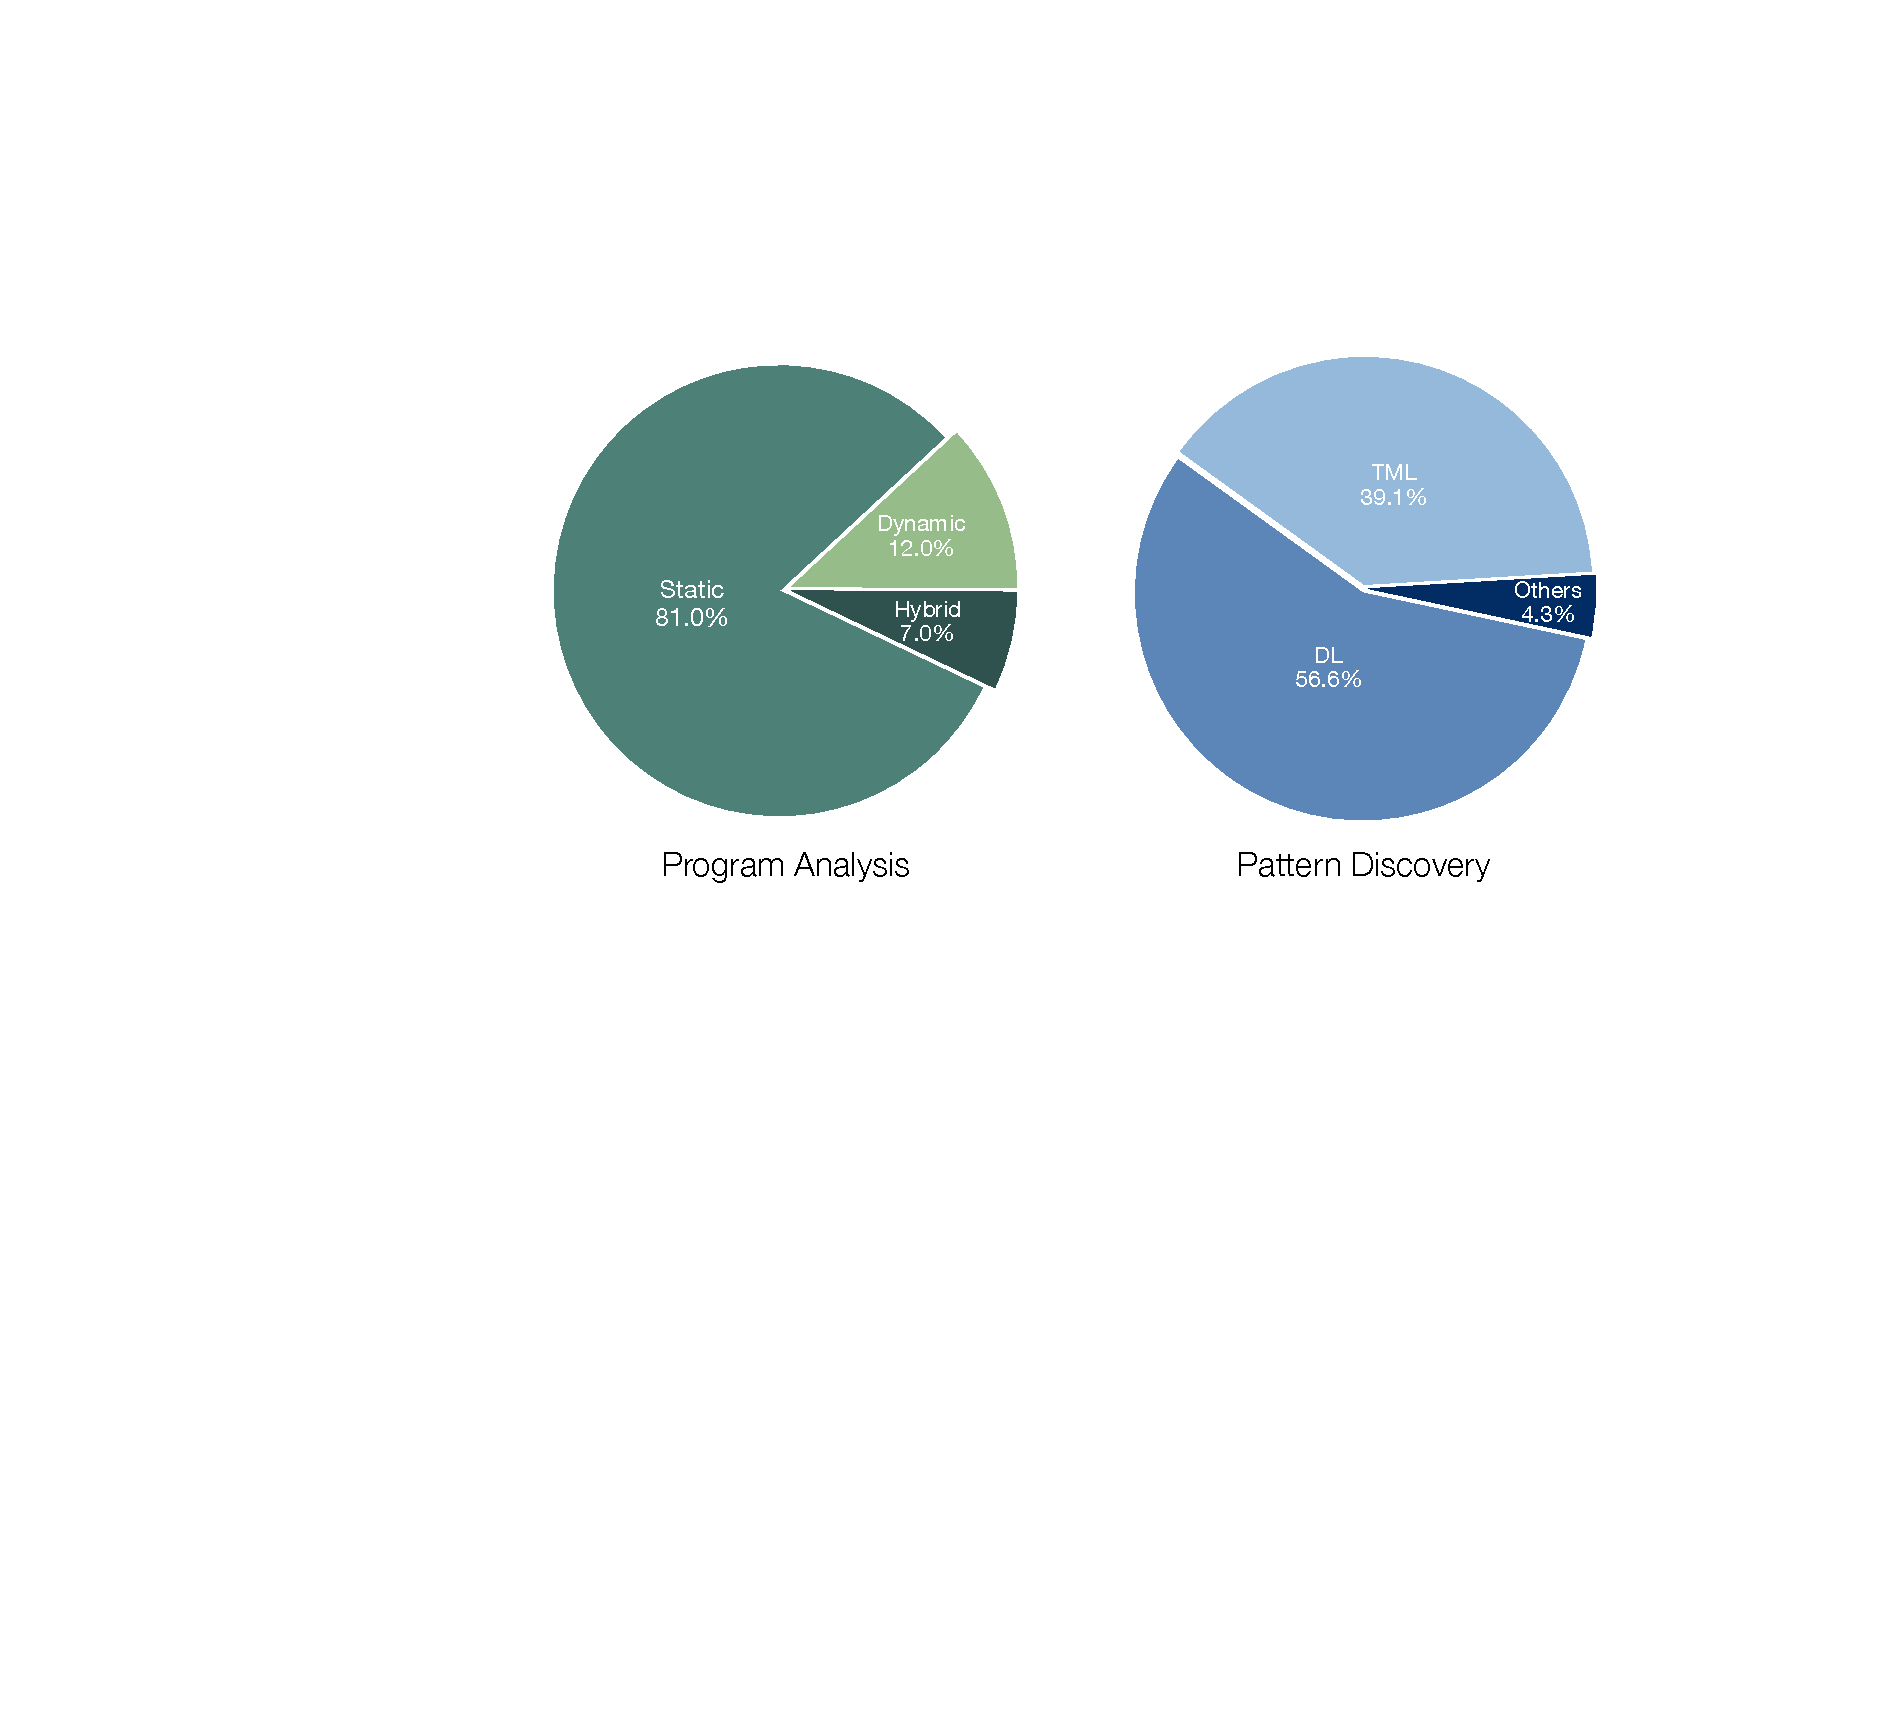
\includegraphics[width=0.73\linewidth]{fig/paper_distribution.pdf}
%     \caption{The overall distribution of investigated approaches from 2011 to 2023.}
%     \label{fig:paper_distribution}
%     \vspace{-0.3cm}
% \end{figure}


% We then categorize these papers based on the program analysis and pattern discovery techniques they employ.
% This distribution of these techniques is illustrated in Figure~\ref{fig:paper_distribution}.
% We observe that \textit{static analysis} emerges as the most favored program analysis technique, followed by \textit{dynamic analysis} and \textit{hybrid analysis}.
% Concurrently, \textit{machine learning (including both traditional machine learning and deep learning)} has been widely used to identify malware patterns.
% This observation further motivates us to focus on ML-based Android malware detection techniques that use static analysis.

\subsection{Feature Database}
\label{sub:feature_db}
To streamline the evaluation of different approaches, we establish a feature database to maintain commonly used features in Android malware detection.
Below, we outline the main features incorporated into the database, categorizing them for ease of reference.
\begin{itemize}[leftmargin=10pt]
    \setlength\itemsep{-1pt}
    \item \textit{Manifest}: this category contains features sourced from the \textit{AndroidManifest.xml} file, such as hardware components, permissions, intents, and app components.
    \item \textit{DisassembledCode}: this category includes the disassembled data extracted from the DEX file, such as the opcode, operands, and code strings.
    \item \textit{ProgramGraph}: this is mainly used to store the program graph of the APK file, including the nodes and edges.
    \item \textit{SharedLibrary}: this category contains the information of the shared libraries used by the APK file.
    \item \textit{Others}: this category includes other features that are not covered by the above categories.
\end{itemize}
Given the structure of the feature database, adding new features becomes straightforward, facilitating the adaptive evaluation of diverse approaches.
For instance, we can easily implement an add-on feature extractor and store the derived features in the database, waiting for use by the preprocessor.

% \vspace{-0.2cm}
% \subsection{\codename Implementation}
% \label{sub:implementation}
% \codename is developed in 17K lines of Python code.
% To ensure consistency and mitigate biases from different feature extraction toolchains and learning frameworks, we adopt standardized techniques across all tasks.
% For feature extraction, we use Androguard~\cite{androguard} to disassemble APK files and derive features such as permissions, intents, and program graphs. 
% LibRadar~\cite{libradar} helps in identifying third-party libraries within the applications, while Angr~\cite{angr} is used for analyzing native libraries and capturing essential features like opcodes and API calls. 
% When it comes to ML models, the scikit-learn library is our choice for traditional ML algorithms like SVM, KNN, and RF.
% On the other hand, for DL architectures such as CNN, GNN, and AE, we resort to Pytorch~\cite{pytorch}.
% This uniform approach ensures a balanced evaluation, concentrating purely on the uniqueness and performance of each method.

% \subsection{\codename Implementation}
% \label{sub:implementation}
% \codename is developed in 17K lines of Python code.
% To ensure consistency and mitigate biases from different feature extraction toolchains and learning frameworks, we adopt standardized techniques across all tasks.
% For feature extraction, we use Androguard~\cite{androguard} to disassemble APK files and derive features such as permissions, intents, and program graphs. 
% LibRadar~\cite{libradar} helps in identifying third-party libraries within the applications, while Angr~\cite{angr} is used for analyzing native libraries and capturing essential features like opcodes and API calls. 
% When it comes to ML models, the scikit-learn library is our choice for traditional ML algorithms like SVM, KNN, and RF.
% On the other hand, for DL architectures such as CNN, GNN, and AE, we resort to Pytorch~\cite{pytorch}.
% This uniform approach ensures a balanced evaluation, concentrating purely on the uniqueness and performance of each method.

\begin{table*}[t]
    \centering
    \caption{
    An overview of the 12 representative approaches we selected from major venues in security, software engineering, and machine learning. 
    \ymark \ indicates that the APK file (\textit{e.g.}, \textit{AndroidManifest.xml} for Manifest) is taken as input in Android malware detection, while \nmark \ is the opposite.
    \cmark \ and \xmark \ indicate whether feature engineering is handcrafted using domain knowledge or learned using representation learning.
    The effectiveness is based on the results reported in the original papers.}
    \vspace{-0.1cm}
    \begin{adjustbox}{width=\linewidth}
    \begin{tabular}{@{}c|cc|cccc|cc|rr|rrr@{}}
    \toprule
    \multirow{2}{*}{\raisebox{-0.3cm}{\textbf{\begin{tabular}[c]{@{}c@{}}Selected \\ Approach\end{tabular}}}} & \multicolumn{2}{c|}{\textbf{Publication}} & \multicolumn{4}{c|}{\textbf{Input from APK}} & \multicolumn{2}{c|}{\textbf{Feature Engineering}} & \multicolumn{2}{c|}{\textbf{Dataset}} & \multicolumn{3}{c}{\textbf{Effectiveness}} \\ \cmidrule(lr){2-3} \cmidrule(lr){4-7} \cmidrule(lr){8-9} \cmidrule(lr){10-11} \cmidrule(l){12-14}
     & \textbf{Venue} & \textbf{Year} & \textbf{Manifest} & \textbf{Dex} & \textbf{Resource} & \textbf{Library} & \textbf{Handcrafted} & \textbf{Learned} & \textbf{Malware} & \textbf{Goodware} & \textbf{TPR} & \textbf{FPR} & \textbf{F1} \\ \midrule
    Drebin\cite{arp2014drebin} & NDSS & 2014 & \ymark & \ymark & \nmark & \nmark & \cmark & \xmark & 5,560 & 123,453 & 94\% & \textbf{1\%} & 87\% \\ \midrule
    % ICCDetector\cite{xu2016iccdetector} & TIFS & 2016 & \ymark & \ymark & \nmark & \nmark & & & 5,264 & 12,026 & 93\% & \textbf{1\%} & 96\% \\ \midrule
    MamaDroid\cite{mariconti2016mamadroid} & NDSS & 2017 & \nmark & \ymark & \nmark & \nmark & \cmark & \xmark & 35,493 & 8,447 & 97\% & 2\% & 96\% \\ \midrule
    Mclaughlin et al.\cite{mclaughlin2017deep} & CODASPY & 2017 & \nmark & \ymark & \nmark & \nmark & \xmark& \cmark & 13,637 & 13,758 & 95\% & \textbf{1\%} & 97\% \\ \midrule
    HinDroid\cite{hou2017hindroid} & KDD & 2017 & \nmark & \ymark & \nmark & \nmark & \cmark & \xmark & 1,216 & 1,118 & \textbf{99\%} & 2\% & \textbf{99\%} \\ \midrule
    DeepRefiner\cite{xu2018deeprefiner} & EuroS\&P & 2018 & \ymark & \ymark & \ymark & \nmark & \xmark & \cmark & 62,915 & 47,525 & 98\% & 2\% & 98\% \\ \midrule
    Kim et al.\cite{kim2018multimodal} & TIFS & 2018 & \ymark & \ymark & \nmark & \ymark & \cmark & \cmark & 21,260 & 20,000 & \textbf{99\%} & \textbf{1\%} & \textbf{99\%} \\ \midrule
    MalScan\cite{wu2019malscan} & ASE & 2019 & \nmark & \ymark & \nmark & \nmark & \cmark & \xmark & 15,430 & 15,285 & --- & --- & 98\% \\ \midrule
    SDAC\cite{xu2020sdac} & TDSC & 2020 & \nmark & \ymark & \nmark & \nmark & \cmark & \cmark & 34,497 & 35,645 & 98\% & \textbf{1\%} & \textbf{99\%}\\ \midrule
    HomDroid\cite{wu2021homdroid} & ISSTA & 2021 & \nmark & \ymark & \nmark & \nmark & \cmark & \xmark & 3,358 & 4,840 & 97\% & 4\% & 95\% \\ \midrule
    Xmal\cite{wu2021android} & TOSEM & 2021 & \ymark & \ymark & \nmark & \nmark & \cmark & \xmark & 15,570 & 20,120 & 98\% & 2\% & 98\% \\ \midrule
    RAMDA\cite{li2021robust} & WWW & 2021 & \ymark & \ymark & \nmark & \nmark & \cmark & \xmark & 21,621 & 36,862 & 93\% & \textbf{1\%} & 90\% \\ \midrule
    MSDroid\cite{he2022msdroid} & TDSC & 2022 & \nmark & \ymark & \nmark & \nmark & \cmark & \xmark & 30,210 & 51,580 & 97\% & \textbf{1\%} & 97\% \\ \bottomrule
    \end{tabular}
    \end{adjustbox}
    \centering
    \begin{tablenotes}
    \footnotesize
    \item \ \ TPR, FPR, and F1 refer to true positive rate, false positive rate, and F1-score. 
    As MalScan is only evaluated on F1, its TPR and FPR are not available.
    \end{tablenotes}
    \label{tab:literature}
    \vspace{-0.3cm}
\end{table*}

\subsection{Reproduction of Selected Approaches}
\label{sub:approach_overview}
Table~\ref{tab:literature} offers a summary of the 12 representative approaches we have selected from leading publications in security~\cite{arp2014drebin,mariconti2016mamadroid,mclaughlin2017deep,xu2018deeprefiner,kim2018multimodal,xu2020sdac,he2022msdroid}, software engineering~\cite{wu2019malscan,wu2021homdroid,wu2021android}, and machine learning~\cite{hou2017hindroid,li2021robust}.
Within this table, we outline the publication details, input from APK, feature engineering style, dataset statistics, and their original effectiveness.
% As highlighted in Section~\ref{sec:discussion}, inconsistencies might exist between our quantitative evaluation results and those previously reported due to various biases, such as datasets, feature extraction toolchains, and learning frameworks.
To better support subsequent research and foster replicability and comparison, we provide the hyper-parameters of these approaches.

\bulletpoint{Drebin}
We replicate Drebin~\cite{arp2014drebin} utilizing a linear SVM with $C=1$, and set max number of iterations to $1000$.

\bulletpoint{MamaDroid}
MamaDroid~\cite{mariconti2016mamadroid} has two abstract mode \textit{i.e.}, package and family.
In our experiments, we choose the family mode, as it is more efficient in terms of time and memory.
For the RF classifier, we employ the default hyper-parameters provided by scikit-learn.

\bulletpoint{Mclaughlin et al}
Mclaughlin et al.~\cite{mclaughlin2017deep} is implemented with a CNN with one single convolutional layer, followed by a max-pooling layer and a fully connected layer.
The convolutional layer is configured with $32$ filters and a kernel size of $225*7$.
The fully connected layer has $16$ neurons.
For the evaluation process, a learning rate of $0.01$ and a batch size of $32$ are employed.
Additionally, inputs that exceed a length of $600000$ are truncated to $60000$, and those that are less than $600000$ are padded with zeros.

\bulletpoint{HinDroid}
In implementing HinDroid~\cite{hou2017hindroid}, various meta-path combinations have been tested. 
$AA^{T}$ yields remarkable performance in our experiments, and hence, is chosen as the meta-path.
For multi-kernel learning, we utilize the $p-norm$ multi-kernel learning framework as released by~\cite{sun2010multiple}, applying the default settings for the hyper-parameters.

\bulletpoint{DeepRefiner}
As discussed in Section~\ref{sub:selected_approaches}, DeepRefiner~\cite{xu2018deeprefiner} has two detection layers, and the second layer shows strong detection capability.
In our experiments, we replicate the second LSTM-based detection layer.
The model configuration is as follows: an embedding size of $16$ for word embeddings (bytecode instructions), a two-layer LSTM model with an input size of $16$, and a hidden size of $64$.
Batch size is set as $32$, and the learning rate is $0.001$.
The input sequence has a maximum length of $50,000$.
Inputs exceeding this length are truncated, while shorter inputs are padded with zeros.

\bulletpoint{Kim et al}
Kim et al.~\cite{kim2018multimodal} initially use a $5$ separated MLPs to process features from five various modalities, each with the same configuration.
Subsequently, a new MLP is introduced to integrate the learned features from the previous MLPs.
The initial five MLPs have layer configurations of $5000, 2500$, and $1000$ neurons.
The last MLP is structured with layers containing $1000, 500, 100$, and $10$ neurons, respectively.
A learning rate of $0.001$ and a batch size of $32$ are used during the training process.

\bulletpoint{MalScan}
The algorithm~\cite{wu2019malscan} is replicated with a KNN classifier, with the number of neighbors set to $3$.

\bulletpoint{SDAC}
SDAC~\cite{xu2020sdac} initially employs Word2Vec to encode API calls into vectors. Following this, K-means clustering is applied, and then these cluster centers are used as anchors to encode features.
In the classification phase, for simplicity, we use a linear SVM instead of multi-voting SVMs.
Additionally, due to K-means's randomness, the algorithm is executed $5$ times, and the average results are computed.
The size of Word2Vec embedding is set as $10$.
The chosen number of clusters is $1000$, and the SVM is configured using default parameters, allowing for $5000$ iterations.

\bulletpoint{HomDroid}
The approach~\cite{wu2021homdroid} is executed using a KNN classifier, with the number of neighbors set to $1$.

\bulletpoint{Xmal}
Xmal~\cite{wu2021android} is implemented using a 3-layer MLP with a hidden size of $64$.
An attention layer is also incorporated, utilizing an MLP with a hidden size of $158$.
The learning rate is set as $0.001$, and the batch size is $20$.

\bulletpoint{RAMDA}
RAMDA~\cite{li2021robust}'s architecture consists of two parts: autoencoder and classifier.
The encoder and decoder each consist of a 3-layer MLP with a hidden size of $600$.
The classifier is a 4-layer MLP with a hidden size of $600$.
During the training process, the autoencoder is trained first, and then the classifier is trained.
Configuration parameters are established with a learning rate of $0.001$, a batch size of $64$, and epochs set at $20$.
A pre-defined reconstruction loss of $30$ is used.
To constrain the loss, the positive weights are defined as $\lambda_1 = 10, \lambda_2 = 1, \lambda_3 = 10$.

\bulletpoint{MSDroid}
MSDroid~\cite{he2022msdroid} is implemented using a 3-layer GNN with a hidden size of $512$.
Subsequent to this, a 2-layer fully connected network with a hidden size of $512$ is used to classify the APKs.
The model's training parameters are set with a learning rate of $0.01$ and a batch size of $64$.

% \begin{figure}[t]
%     \centering
%     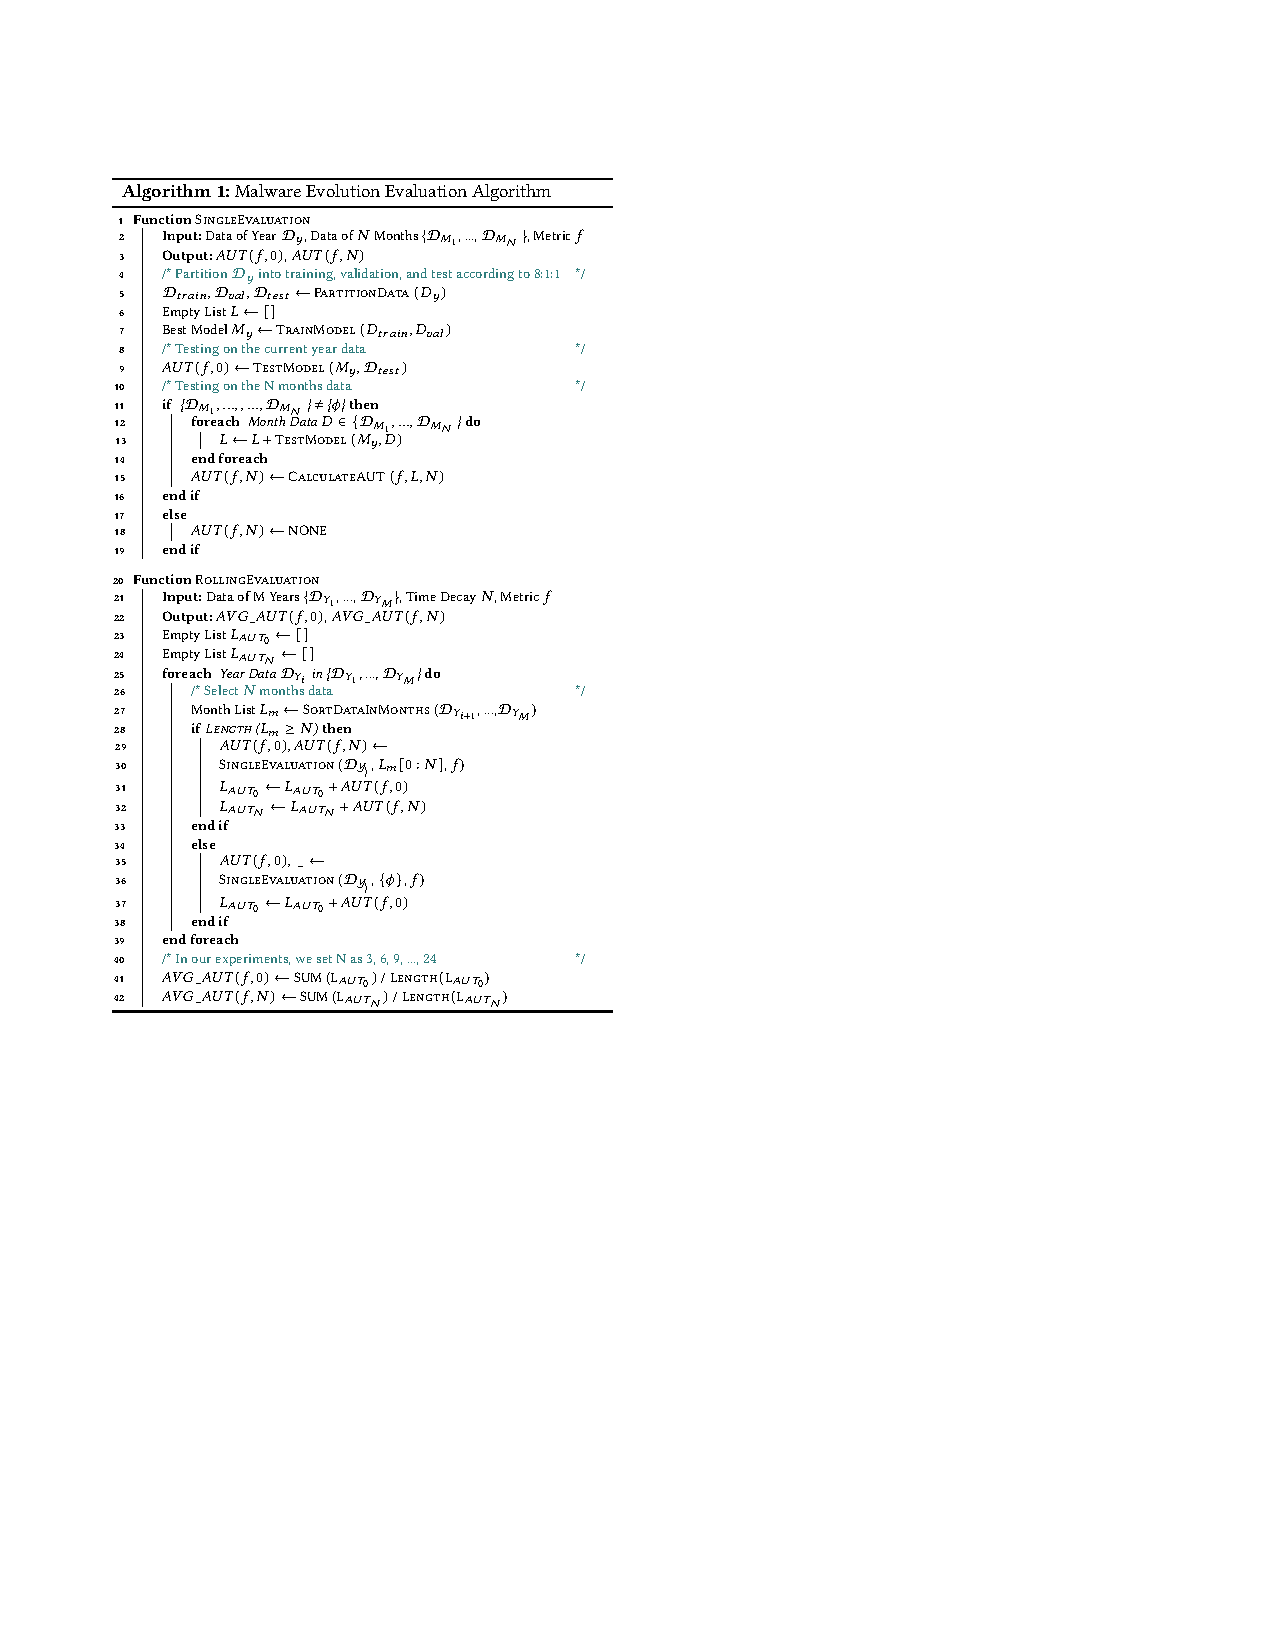
\includegraphics[width=0.86\linewidth]{fig/algorithm.pdf}
%     % \vspace{-0.3cm}
%     \caption{The rolling algorithm for evaluating the Android malware evolution.}
%     \label{fig:evolution_algorithm}
%     \vspace{-0.5cm}
% \end{figure}



\begin{table*}[t]
    \centering
    \renewcommand{\arraystretch}{1.1}
    \caption{The AUT(TPR, N) and AUT(FRP, N) of the selected approaches over varying time decays. In this analysis, we examine the shifts during various malware evolution periods: 3, 6, 9, 12, 15, 18, 21, and 24 months.}
    \vspace{-0.1cm}
    \begin{adjustbox}{width=\textwidth}
        \begin{tabular}{@{}c|c|c|c|c|c|c|c|c|c@{}}
            \toprule
            \textbf{Approach}         & \textbf{AUT(TPR,0)} & \textbf{AUT(TPR,3)} & \textbf{AUT(TPR,6)} & \textbf{AUT(TPR,9)} & \textbf{AUT(TPR,12)} & \textbf{AUT(TPR,15)} & \textbf{AUT(TPR,18)} & \textbf{AUT(TPR,21)} & \textbf{AUT(TPR,24)} \\ \midrule
            Drebin            & 0.803               & 0.722(-10.1\%)      & 0.670(-16.5\%)      & 0.601(-25.1\%)      & 0.564(-29.8\%)       & 0.530(-34.0\%)       & 0.508(-36.7\%)       & 0.484(-39.7\%)       & 0.466(-41.9\%)       \\ \midrule
            MamaDroid         & 0.712               & 0.496(-30.3\%)      & 0.429(-39.7\%)      & 0.365(-48.7\%)      & 0.322(-54.7\%)       & 0.308(-56.7\%)       & 0.282(-60.4\%)       & 0.253(-64.5\%)       & 0.233(-67.2\%)       \\ \midrule
            Mclaughlin et al. & 0.724               & 0.583(-19.6\%)      & 0.526(-27.3\%)      & 0.461(-36.4\%)      & 0.410(-43.4\%)       & 0.378(-47.9\%)       & 0.354(-51.2\%)       & 0.327(-54.9\%)       & 0.303(-58.1\%)       \\ \midrule
            HinDroid          & 0.831               & 0.786(-5.5\%)       & 0.773(-7.0\%)       & 0.729(-12.3\%)      & 0.687(-17.4\%)       & 0.684(-17.8\%)       & 0.674(-19.0\%)       & 0.662(-20.3\%)       & 0.655(-21.2\%)       \\ \midrule
            DeepRefiner       & 0.774               & 0.590(-23.7\%)      & 0.545(-29.6\%)      & 0.478(-38.3\%)      & 0.427(-44.8\%)       & 0.413(-46.6\%)       & 0.388(-49.9\%)       & 0.362(-53.2\%)       & 0.339(-56.2\%)       \\ \midrule
            Kim et al.        & 0.845               & 0.760(-10.0\%)      & 0.745(-11.8\%)      & 0.676(-20.0\%)      & 0.619(-26.7\%)       & 0.583(-31.0\%)       & 0.557(-34.0\%)       & 0.524(-38.0\%)       & 0.49(-42.0\%)        \\ \midrule
            MalScan           & 0.800               & 0.685(-14.4\%)      & 0.650(-18.8\%)      & 0.584(-27.0\%)      & 0.547(-31.6\%)       & 0.519(-35.2\%)       & 0.494(-38.3\%)       & 0.465(-41.8\%)       & 0.439(-45.1\%)       \\ \midrule
            SDAC              & 0.734               & 0.616(-16.1\%)      & 0.554(-24.5\%)      & 0.495(-32.6\%)      & 0.455(-38.0\%)       & 0.439(-40.2\%)       & 0.416(-43.4\%)       & 0.391(-46.8\%)       & 0.369(-49.7\%)       \\ \midrule
            HomDroid          & 0.836               & 0.689(-17.5\%)      & 0.651(-22.1\%)      & 0.596(-28.7\%)      & 0.546(-34.6\%)       & 0.515(-38.4\%)       & 0.486(-41.8\%)       & 0.448(-46.4\%)       & 0.422(-49.5\%)       \\ \midrule
            Xmal              & 0.836               & 0.741(-11.3\%)      & 0.693(-17.1\%)      & 0.617(-26.1\%)      & 0.575(-31.2\%)       & 0.550(-34.2\%)       & 0.523(-37.4\%)       & 0.492(-41.2\%)       & 0.463(-44.6\%)       \\ \midrule
            RAMDA             & 0.876               & 0.814(-7.0\%)       & 0.775(-11.6\%)      & 0.733(-16.3\%)      & 0.689(-21.3\%)       & 0.673(-23.2\%)       & 0.658(-24.8\%)       & 0.637(-27.2\%)       & 0.613(-30.1\%)       \\ \midrule
            MSDroid           & 0.835               & 0.755(-9.6\%)       & 0.732(-12.3\%)      & 0.673(-19.4\%)      & 0.635(-24.0\%)       & 0.632(-24.3\%)       & 0.604(-27.6\%)       & 0.569(-31.9\%)       & 0.544(-34.8\%)       \\ \midrule \midrule

            \textbf{Approach}         & \textbf{AUT(FPR,0)} & \textbf{AUT(FPR,3)} & \textbf{AUT(FPR,6)} & \textbf{AUT(FPR,9)} & \textbf{AUT(FPR,12)} & \textbf{AUT(FPR,15)} & \textbf{AUT(FPR,18)} & \textbf{AUT(FPR,21)} & \textbf{AUT(FPR,24)} \\ \midrule
            Drebin            & 0.014               & 0.02(+42.2\%)       & 0.023(+68.2\%)      & 0.024(+71.1\%)      & 0.026(+85.6\%)       & 0.029(+110.1\%)      & 0.030(+115.2\%)      & 0.031(+126.7\%)      & 0.033(+141.2\%)      \\ \midrule
            MamaDroid         & 0.009               & 0.010(+17.9\%)      & 0.011(+28.4\%)      & 0.010(+20.2\%)      & 0.011(+31.9\%)       & 0.013(+50.5\%)       & 0.013(+54.0\%)       & 0.014(+62.2\%)       & 0.014(+59.9\%)       \\ \midrule
            Mclaughlin et al. & 0.013               & 0.010(-19.1\%)      & 0.012(-7.5\%)       & 0.013(+1.9\%)       & 0.015(+14.3\%)       & 0.016(+23.6\%)       & 0.016(+24.4\%)       & 0.016(+22.1\%)       & 0.016(+20.5\%)       \\ \midrule
            HinDroid          & 0.016               & 0.262(+1491.6\%)    & 0.266(+1516.6\%)    & 0.271(+1548.8\%)    & 0.279(+1599.3\%)     & 0.319(+1839.1\%)     & 0.321(+1853.7\%)     & 0.324(+1873.8\%)     & 0.327(+1890.3\%)     \\ \midrule
            DeepRefiner       & 0.017               & 0.019(+9.3\%)       & 0.018(+5.9\%)       & 0.019(+7.6\%)       & 0.021(+20.3\%)       & 0.022(+27.2\%)       & 0.022(+28.9\%)       & 0.023(+31.2\%)       & 0.024(+38.7\%)       \\ \midrule
            Kim et al.        & 0.014               & 0.017(+19.7\%)      & 0.018(+29.8\%)      & 0.018(+31.9\%)      & 0.02(+43.5\%)        & 0.024(+75.9\%)       & 0.026(+84.6\%)       & 0.027(+91.8\%)       & 0.027(+95.4\%)       \\ \midrule
            MalScan           & 0.025               & 0.029(+17.1\%)      & 0.029(+18.7\%)      & 0.029(+17.9\%)      & 0.031(+24.8\%)       & 0.031(+26.1\%)       & 0.033(+33.0\%)       & 0.035(+40.7\%)       & 0.037(+50.1\%)       \\ \midrule
            SDAC              & 0.024               & 0.042(+72.1\%)      & 0.050(+104.4\%)     & 0.054(+121.6\%)     & 0.060(+146.5\%)      & 0.064(+159.6\%)      & 0.066(+169.9\%)      & 0.068(+176\%)        & 0.072(+192.3\%)      \\ \midrule
            HomDroid          & 0.014               & 0.023(+63.2\%)      & 0.024(+66.0\%)      & 0.023(+59.0\%)      & 0.024(+66.0\%)       & 0.026(+78.5\%)       & 0.028(+94.6\%)       & 0.031(+112.7\%)      & 0.032(+123.8\%)      \\ \midrule
            Xmal              & 0.023               & 0.025(+11.6\%)      & 0.028(+23.5\%)      & 0.027(+20.4\%)      & 0.027(+18.2\%)       & 0.028(+21.7\%)       & 0.028(+25.3\%)       & 0.029(+28.4\%)       & 0.030(+30.6\%)       \\ \midrule
            RAMDA             & 0.054               & 0.061(+14.0\%)      & 0.069(+27.6\%)      & 0.075(+38.7\%)      & 0.081(+50.0\%)       & 0.09(+67.1\%)        & 0.093(+73.4\%)       & 0.099(+84.2\%)       & 0.104(+93.9\%)       \\ \midrule
            MSDroid           & 0.072               & 0.078(+8.4\%)       & 0.080(+11.7\%)      & 0.082(+14.5\%)      & 0.085(+18.4\%)       & 0.093(+29.2\%)       & 0.098(+37.3\%)       & 0.106(+47.4\%)       & 0.111(+55.1\%)       \\ \bottomrule
            \end{tabular}
    \end{adjustbox}
    \label{tab:tpr_time_decay}
    \vspace{-0.3cm}  
\end{table*}

\begin{table}[t]
    \centering
    \renewcommand{\arraystretch}{0.6}
    \caption{The effectiveness of the selected approaches using different size training data.}
    \vspace{-0.1cm}
    \begin{adjustbox}{width=0.54\linewidth}
    \begin{tabular}{@{}c|c|c|c@{}}
    \toprule
    \diagbox[innerleftsep=-0.1em, innerrightsep=-0.2em, height=2.6em,width=7em]{\textbf{Approach}}{\textbf{Data Size}} & \textbf{100\%} & \textbf{50\%}& \textbf{10\%}\\ \midrule
    Drebin& 0.722 & 0.714 (-1.2\%) & 0.643 (-10.9\%) \\ \midrule
    MamaDroid& 0.661 & 0.623 (-5.7\%) & 0.452 (-31.5\%) \\ \midrule
    Mclaughlin et al.& 0.714 & 0.627 (-12.2\%) & 0.140 (-80.4\%) \\ \midrule
    HinDroid & 0.731 & 0.716 (-2.0\%) & 0.618 (-15.5\%) \\ \midrule
    DeepRefiner& 0.657 & 0.577 (-12.1\%) & 0.327 (-50.2\%) \\ \midrule
    Kim et al. & 0.782 & 0.742 (-5.1\%) & 0.611 (-21.8\%) \\ \midrule
    MalScan& 0.684 & 0.653 (-4.6\%) & 0.526 (-23.1\%) \\ \midrule
    SDAC & 0.522 & 0.496 (-5.0\%) & 0.474 (-9.1\%) \\ \midrule
    HomDroid& 0.734 & 0.675 (-8.0\%) & 0.586 (-20.1\%) \\ \midrule
    Xmal& 0.698 & 0.668 (-4.2\%) & 0.613 (-12.2\%) \\ \midrule
    RAMDA& 0.636 & 0.614 (-3.4\%) & 0.547 (-14.0\%) \\ \midrule
    MSDroid& 0.648 & 0.563 (-13.0\%) & 0.424 (-34.6\%) \\ \bottomrule
    \end{tabular}
    \end{adjustbox}
    \label{tab:res_training_size}
    \vspace{-0.3cm}
\end{table}

\subsection{AUT, ASR, and APR}
\label{sub:aut}
In assessing a classifier's resilience against temporal degradation, we employ the Area Under Time (AUT) metric as suggested by~\cite{pendlebury2019tesseract}.
AUT is formally given by:
$$
AUT(f, N) = \frac{1}{N-1}\sum_{k=1}^{N-1}\frac{f(k+1)+f(k)}{2},
$$
where $f$ represents the chosen performance metric (such as F1 score or True Positive Rate) and $N$ denotes the count of malware evolution period. 
AUT values range between $(0,1)$, where 1 indicates the classifier retains consistent performance across time.

To evaluate a classifier's robustness against adversarial attacks, we use two primary metrics: the attack success rate (ASR) and average perturbation ratio (APR) metrics utilized by~\cite{li2023black}.
They are mathematically defined as:
$$
ASR = \frac{N_{success}}{N_{total}}, \ APR = \frac{F_{modified}}{F_{total}}.
$$
Here, $N_{success}$ refers to the number of adversarial examples that successfully deceive the classifier.
$N_{total}$ represents the entire set of adversarial samples.
Meanwhile, $F_{modified}$ is the number of input features changed by the adversarial intervention, and $F_{total}$ signifies the total number of features in the input.
The ASR values fall within the interval $(0,1)$; a value of 1 suggests the classifier is entirely susceptible to adversarial attacks.
Similarly, APR values lie within $(0,1)$.
A higher APR indicates that evading the classifier becomes increasingly challenging.

% \vspace{-0.2cm}
% \subsection{Malware Evolution Algorithm}
% \label{sub:malware_evolution_algorithm}
% To evaluate the evolution of Android malware, we propose a rolling algorithm, as illustrated in Figure~\ref{fig:evolution_algorithm}.
% In our experiment, we use the data from 2011 to 2020, and the malware evolution periods are set as 3, 6, 9, 12, 15, 18, 21, and 24 months.

% \vspace{-0.2cm}
\subsection{Additional Results}
\label{sec:additional_results}
Table~\ref{tab:res_training_size} presents the detailed results of training data size analysis.
In Sec.~\ref{effectiveness}, we normalize the results of the selected approaches based on the use of 100\% training data size for clarity.
For instance, the normalized result for Drebin, using 50\% of the training data, is computed as $\frac{0.714}{0.722} = 0.988$.
These results highlight the significant impact that the volume of data has on the effectiveness of the selected approaches.

For the analysis of malware evolution, the results of AUT(TPR, N) and AUT(FPR, N) are reported in Table~\ref{tab:tpr_time_decay} (N is also set as 0, 3, 6, 9, 12, 15, 18, 21, and 24 months).
We observe that as malware evolution time increases, there is a consistent decrease in AUT(TPR, N) for the selected approaches.
This trend suggests that as malware evolves, more malware samples are misclassified as benign.
Simultaneously, an increase in AUT(FPR, N) is noted, indicating that more benign samples are misclassified as malware.
Overall, the performance of malware detection approaches degrades with the increase of malware evolution time.

\end{document}
\endinput
